
\documentclass[12pt,a4paper,oneside]{ctexbook}
\usepackage{physics} % for \ket, \bra, \expval, etc.
\usepackage{graphicx}
\usepackage{lmodern}
\usepackage{amssymb,amsmath}
\usepackage{hyperref}
\usepackage{ifxetex,ifluatex}
\usepackage{fixltx2e} % provides \textsubscript
\usepackage{enumitem}
\usepackage{bm}

\ctexset{
  section = {
    name = {},
    number = \Roman{section},
    format = \normalfont\bfseries\Large,
    aftername = {.~},
    beforeskip = 1ex plus 0.2ex minus 0.1ex,
    afterskip = 0.5ex plus 0.1ex,
  },
  subsection = {
    name = {},
    number = \Alph{subsection},
    format = \normalfont\bfseries\large,
    aftername = {.~},
  },
  subsubsection = {
    name = {},
    number = \arabic{subsubsection},
    format = \normalfont\bfseries\normalsize,
    aftername = {.~},
  },
  paragraph = {
    name = {},
    number = \alph{paragraph},
    format = \normalfont\itshape,
    aftername = {.~},
    runin = true,  % 行内标题
    aftertitle = {.},  % 标题后加句点
  },
  subparagraph = {
    name = {},
    number = \roman{subparagraph},
    format = \normalfont\itshape,
    aftername = {.~},
    runin = true,  % 行内标题
    aftertitle = {.},  % 标题后加句点
  },
}

\setcounter{secnumdepth}{3}
\setcounter{tocdepth}{3}
\setlength{\parskip}{0.4em}
\setlength{\parindent}{2em}
% 设置编号深度
\setcounter{secnumdepth}{4}

\pagestyle{plain} % 统一页码位置（底部居中）

\hypersetup{
    colorlinks=true,
    linkcolor=blue,
    citecolor=blue,
    urlcolor=blue,
    pdfstartview=FitH
}

\title{Notes on SQC}
\author{Zip}
\date{\today}
\begin{document}

\frontmatter            % 前言区：页码 i, ii, iii...（可选）
\maketitle
\tableofcontents

\mainmatter             % 正文：页码从 1 开始






\section{I. 引言（Introduction）}

\subsection{量子计算发展的整体背景}

文章开篇首先从宏观背景切入，指出在过去十年中，\textbf{量子计算}与\textbf{量子信息科学}在学术界和工业界都获得了巨大的发展动能。伴随着这种持续的推动，理论与实验两条主线都在快速前进，使得量子计算逐渐从一种“数学上的好奇心”转变为一个\textbf{快速发展的创新领域}。

作者特别强调，近年来在不同物理体系中，围绕量子系统及其纠缠性质已经取得了显著进展，主要集中在以下三个方面：
\begin{enumerate}[leftmargin=2em]
    \item \textbf{量子态或量子系统的创建（creation）}；
    \item \textbf{量子系统的控制（control）}；
    \item \textbf{量子系统的测量（measurement）}。
\end{enumerate}

这三种能力构成了量子实验平台最核心的基础能力链条：
\[
\text{创建} \;\to\; \text{控制} \;\to\; \text{测量}.
\]
文章的出发点正是在这样的大背景下展开：量子计算已不再只是概念层面的探索，而是正在进入以实验实现和系统工程为中心的快速推进阶段。

\subsection{为什么 cQED 是核心平台之一}

在众多量子计算实现路线中，作者特别强调了\textbf{电路量子电动力学（circuit quantum electrodynamics, cQED）}的重要地位。文章指出，cQED 已经成为实现\textbf{鲁棒的（robust）}、\textbf{可扩展的（scalable）}、\textbf{通用量子计算机（universal quantum computer）}最有前景的平台之一。

作者作出这一判断，并非仅仅因为 cQED 在理论上具备潜力，而是因为它已经支撑了一系列具有里程碑意义的实验成果，例如：
\begin{itemize}[leftmargin=2em]
    \item \textbf{量子纠错（quantum error correction）的首次实现之一}；
    \item \textbf{量子处理器相对于经典对应物展现潜在量子优势（quantum advantage）的实验展示}。
\end{itemize}

因此，cQED 的重要性体现在两个层面：
\begin{enumerate}[leftmargin=2em]
    \item 它在原理上适合构建可扩展的量子系统；
    \item 它在实验上已经产生了具有代表性的关键成果。
\end{enumerate}

\subsection{cQED 的基本定义与物理优势}

\subsubsection{cQED 的基本含义}

文章对 cQED 给出了一个简洁而关键的定义：从本质上讲，cQED 描述的是\textbf{光与物质的相互作用}，其中：
\begin{itemize}[leftmargin=2em]
    \item 光通常对应\textbf{微波频段的电磁场}；
    \item 物质则由\textbf{超导电路元件}构成。
\end{itemize}

因此，可以将 cQED 理解为：
\[
\text{微波光场} + \text{超导电路元件}
\;\longrightarrow\;
\text{可工程化的量子系统}.
\]

\subsubsection{cQED 平台的突出特征}

作者强调，cQED 器件中的各组成部分具有\textbf{高度可配置性（highly configurable）}，这意味着研究者可以按需设计系统参数，而不仅仅被材料本征属性所限制。

这种平台的优势主要体现在两个方面：
\begin{enumerate}[leftmargin=2em]
    \item \textbf{能够提供大且可控的非线性（large, controllable nonlinearities）}，从而支持\textbf{快速量子操作}；
    \item \textbf{能够较好地与环境隔离（isolation from the environment）}，从而维持\textbf{稳健的量子相干性（robust quantum coherence）}。
\end{enumerate}

这实际上说明，cQED 的工程价值在于它试图同时兼顾以下两个目标：
\[
\text{强可控性} \qquad \text{与} \qquad \text{高相干性}.
\]
而在量子硬件中，这两者通常是最关键、也最难平衡的要求。

\subsubsection{构建 cQED 量子处理器的要求}

文章进一步指出，构建一个 cQED 量子处理器，并不仅仅是设计和制造芯片这么简单，而是需要同时推进两类工作：
\begin{itemize}[leftmargin=2em]
    \item \textbf{器件设计与制备（design and fabrication）}；
    \item \textbf{测量与控制系统的持续优化（measurement and control setup optimization）}。
\end{itemize}

这意味着 cQED 的实现本质上是一个\textbf{全栈工程问题}，而不是某一个单独元件的问题。为了真正构建大规模通用量子计算机，技术栈中的每一个层级都必须经过精细设计，并在持续研究和创新中不断改进。

\subsection{本文的定位、目标读者与写作动机}

\subsubsection{为什么还需要这篇 Tutorial}

作者指出，随着 cQED 技术逐渐成熟，其每一个组成部分的实现都变得越来越：
\begin{itemize}[leftmargin=2em]
    \item \textbf{复杂（sophisticated）}；
    \item \textbf{多学科交叉（multidisciplinary）}。
\end{itemize}

虽然该领域已经存在许多高水平综述文章，它们通常能够系统总结若干关键方向上的最新进展，并为专家读者提供全面视角，但作者认为，这些综述大多更适合已有经验的研究者，而未必适合刚进入实验领域的新手。

因此，本文的写作动机是：为处于起步阶段的实验研究者提供一篇更偏向\textbf{实践工作流}和\textbf{实验实现细节}的 Tutorial。

\subsubsection{目标读者}

文章明确将本文定位为一篇\textbf{入门型实验教程}，主要面向：
\begin{quote}
\textbf{刚刚开始搭建超导量子系统的实验研究者。}
\end{quote}

也就是说，本文不是写给已经长期深耕该领域、熟悉全部技术路线和实验技巧的专家，而是写给希望理解“如何真正把 cQED 系统做出来”的初学者和新进入者。

\subsubsection{与已有教学性综述的区别}

作者还将本文与已有教学性综述进行对比，指出本文的重点不在于构建一个尽可能完整的 cQED 知识体系，而在于更加聚焦于：
\begin{itemize}[leftmargin=2em]
    \item \textbf{超导量子器件搭建过程中真正需要用到的实验技术}；
    \item \textbf{具体实验实践中积累出来的方法与经验}；
    \item \textbf{对新手尤其关键的工具与直觉}。
\end{itemize}

因此，本文的特点不是“面面俱到”，而是“强调实操”。

\subsubsection{本文的核心目标}

作者明确说明，本文并不意图成为：
\begin{itemize}[leftmargin=2em]
    \item 整个 cQED 领域的全面综述；
    \item 社区中全部技术路线和方法的穷尽式总结。
\end{itemize}

相反，本文的目标是讨论一组作者认为\textbf{最基础、最有用、最能帮助理解 cQED 实验实现过程的工具与直觉}。具体而言，作者希望做到：
\begin{enumerate}[leftmargin=2em]
    \item 以 Tutorial 的形式，带领读者走完 cQED 器件设计与表征的基本流程；
    \item 对工作流中的其他重要环节给出较为概括的介绍；
    \item 提供对后续深入学习有帮助的参考线索；
    \item 重点聚焦于\textbf{采用 transmon 量子比特的器件}。
\end{enumerate}

因此，本文可以理解为：
\[
\text{以设计与表征为主线的实验入门教程}
\;+\;
\text{对相关环节的工作流式概览}.
\]

\subsection{图1：文章所强调的核心工程图景}
\begin{figure}[htbp]
    \centering
    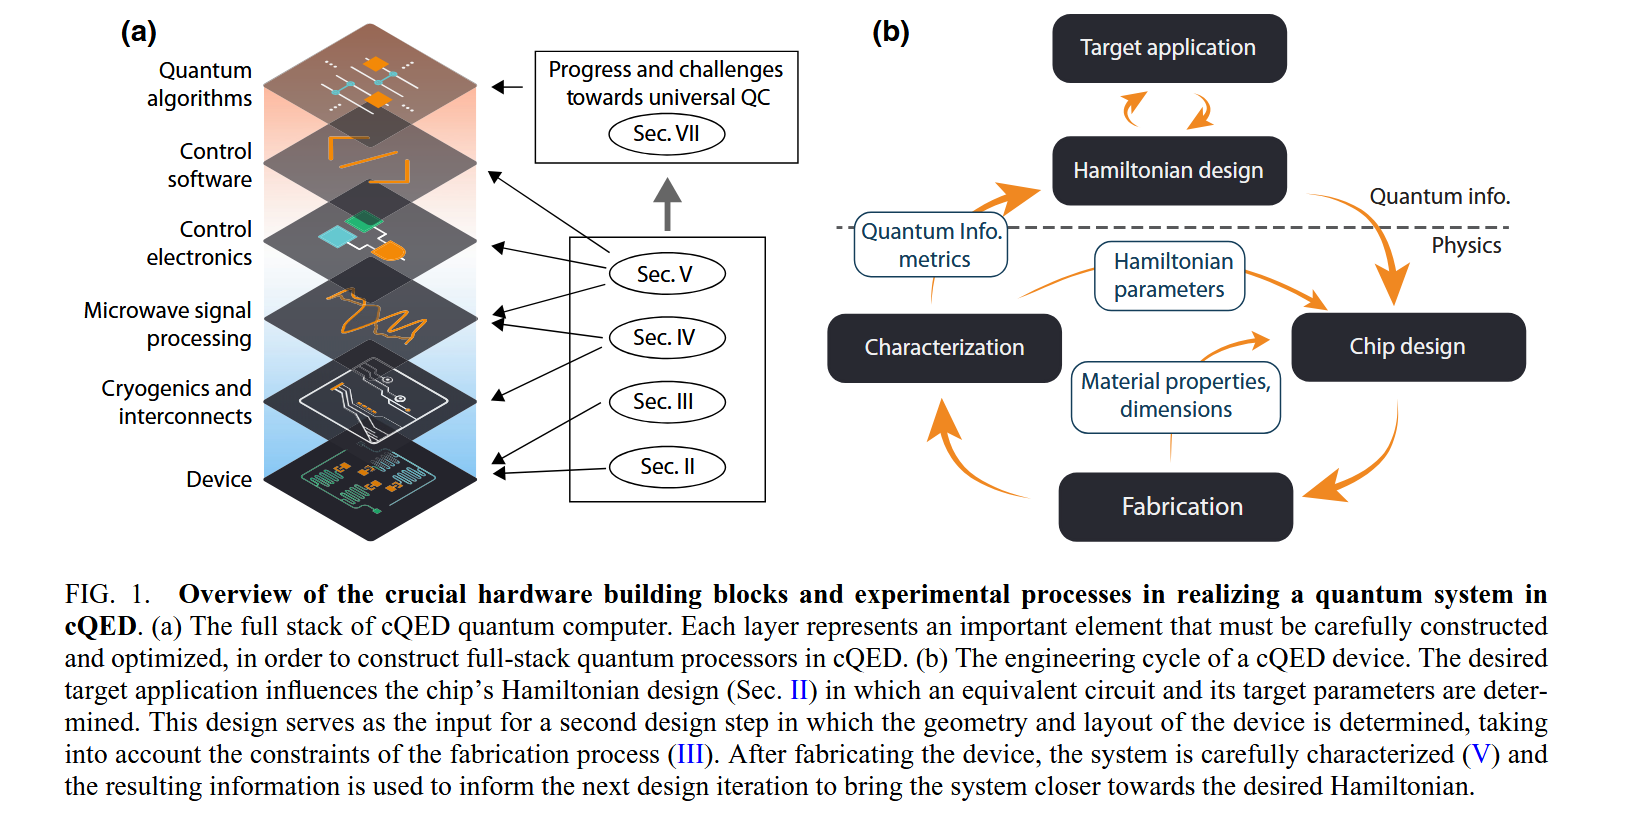
\includegraphics[width=0.9\textwidth]{img/overview.png}
    \caption{(a) cQED 量子计算机的全栈结构示意图；(b) cQED 器件开发的工程闭环示意图。}
    \label{fig:figure1}
\end{figure}
\subsubsection{图1(a)：cQED 量子计算机的全栈结构}

图1(a) 给出了 cQED 量子计算机的\textbf{全栈结构示意图}。从下到上，图中展示了如下层级：
\begin{enumerate}[leftmargin=2em]
    \item \textbf{Device}（器件）；
    \item \textbf{Cryogenics and interconnects}（低温系统与互连）；
    \item \textbf{Microwave signal processing}（微波信号处理）；
    \item \textbf{Control electronics}（控制电子学）；
    \item \textbf{Control software}（控制软件）；
    \item \textbf{Quantum algorithms}（量子算法）。
\end{enumerate}

图注说明，这些层级共同构成了一个 cQED 全栈量子处理器。每一层都不是可有可无的配套部分，而是实现完整量子系统时必须认真设计和优化的关键要素。

这张图传达出几个核心认识：
\begin{itemize}[leftmargin=2em]
    \item 量子计算不是单一芯片问题，而是\textbf{系统工程问题}；
    \item 从底层器件到高层软件与算法，各层之间存在强耦合关系；
    \item 任一层级性能不足，都会限制整体系统表现；
    \item 真正的可扩展量子计算，要求\textbf{全栈协同优化}。
\end{itemize}

图中还通过章节编号将这些层级与后文内容联系起来，体现出本文并不是碎片化介绍若干知识点，而是围绕一个完整实验系统的不同层次逐步展开。

\subsubsection{图1(b)：cQED 器件开发的工程闭环}

图1(b) 展示了一个 cQED 器件开发的\textbf{工程闭环（engineering cycle）}，其核心流程为：
\[
\text{Target application}
\;\to\;
\text{Hamiltonian design}
\;\to\;
\text{Chip design}
\;\to\;
\text{Fabrication}
\;\to\;
\text{Characterization}
\;\to\;
\text{反馈到下一轮设计}.
\]

图中涉及的主要模块包括：
\begin{itemize}[leftmargin=2em]
    \item \textbf{Target application}（目标应用）；
    \item \textbf{Hamiltonian design}（哈密顿量设计）；
    \item \textbf{Chip design}（芯片设计）；
    \item \textbf{Fabrication}（制备）；
    \item \textbf{Characterization}（表征）。
\end{itemize}

此外，图中还标出了几个连接不同层级的信息对象：
\begin{itemize}[leftmargin=2em]
    \item \textbf{Quantum info. metrics}（量子信息指标）；
    \item \textbf{Hamiltonian parameters}（哈密顿量参数）；
    \item \textbf{Material properties, dimensions}（材料性质与几何尺寸）。
\end{itemize}

这一工程循环反映了 cQED 器件设计的基本逻辑：

\begin{enumerate}[leftmargin=2em]
    \item \textbf{先确定目标应用。} \\
    器件设计不是从“画芯片”开始，而是从要完成什么量子信息任务开始。

    \item \textbf{再根据应用要求设计哈密顿量。} \\
    目标应用决定所需的有效模型、频率结构、耦合关系和性能指标。

    \item \textbf{将哈密顿量参数落实为真实芯片结构。} \\
    理论上的参数必须进一步映射为具体的几何、版图和器件构型。

    \item \textbf{设计必须服从制备工艺约束。} \\
    芯片设计不是纯理论过程，还必须考虑材料性质、尺寸公差和工艺窗口。

    \item \textbf{制备之后必须进行系统表征。} \\
    器件做出来并不代表设计目标已经实现，还需要通过实验测量确定其真实参数和性能。

    \item \textbf{表征结果将反馈到下一轮设计。} \\
    因而，器件开发不是一次性流程，而是持续迭代逼近期望哈密顿量的工程过程。
\end{enumerate}

\subsubsection{图中的“Quantum info.”与“Physics”分界}

图1(b) 中通过虚线区分了“Quantum info.”与“Physics”两个层面，这一设计强调了 cQED 工程中的核心桥梁作用：

\begin{quote}
\textbf{上层的量子信息目标，必须通过下层的物理参数、材料性质、几何结构和工艺流程才能真正实现。}
\end{quote}

这意味着量子信息中的抽象目标不会自动转化为器件性能，中间必须经过从目标、模型、设计、制造到测量验证的完整映射链条。

\subsection{A. Overview of article：全文工作流与章节安排}

\subsubsection{整体组织方式}

作者指出，本文的组织方式仿照的是\textbf{在实验室中搭建一个新的 cQED 实验平台的完整工作流}。因此，文章不是按纯粹理论主题分类，而是尽量贴近真实实验的推进过程。

这样组织的原因在于：
\begin{enumerate}[leftmargin=2em]
    \item 搭建 cQED 平台是一个多步骤流程；
    \item 每一步都对最终实现鲁棒量子器件至关重要；
    \item 许多实验中非常关键的实践细节，往往会在研究论文中被简略处理甚至省略。
\end{enumerate}

因此，本文希望提供的是一种\textbf{逐步展开的实践性路线图}。

\subsubsection{第二节的作用：建立共同的物理基础}

作者说明，文章首先会在第二节对 cQED 的物理学作一个简明总结。其作用有两个：
\begin{itemize}[leftmargin=2em]
    \item 为后续关于设计、表征、控制等讨论建立共同的物理基础；
    \item 为想要进一步深入的读者提供继续学习更高阶概念的资源入口。
\end{itemize}

因此，第二节在全文中的定位可以概括为：
\[
\text{后续实验与工程讨论的理论底座}.
\]

\subsubsection{第三节：从目标哈密顿量到真实物理电路}

第三节将讨论一个非常关键的问题，即如何把\textbf{目标哈密顿量（target Hamiltonian）}转化为一个真实可制造的物理电路。

作者指出，这一过程是一个\textbf{迭代循环}，主要包括以下几个步骤：
\begin{enumerate}[leftmargin=2em]
    \item \textbf{配置器件布局和电路元件}；
    \item \textbf{模拟电磁模结构}；
    \item \textbf{提取相关哈密顿量参数}。
\end{enumerate}

除此之外，第三节还会进一步讨论：
\begin{itemize}[leftmargin=2em]
    \item 当前量子电路相干性的主要限制因素；
    \item 已知的相干性缓解设计策略；
    \item 器件制备中的若干问题；
    \item 实现更高\textbf{良率（yield）}和\textbf{可靠性（reliability）}的考虑。
\end{itemize}

因此，第三节不仅处理“如何设计一个器件”，还处理“如何设计一个性能可靠、可制造、可复现的器件”。

\subsubsection{第四节：低温环境、室温环境与控制链路}

第四节从器件层面转向\textbf{实验环境与控制系统}。作者强调，为了同时保证 cQED 器件的\textbf{相干性}和\textbf{可控性}，必须认真搭建从低温端到室温端的整套实验环境。

这一节包括两个重点方向：

\begin{enumerate}[leftmargin=2em]
    \item \textbf{低温环境：}介绍在\textbf{稀释制冷机（dilution refrigerator, DR）}中保证量子器件稳定工作的关键因素，特别是\textbf{滤波（filtering）}与\textbf{屏蔽（shielding）}；
    \item \textbf{室温环境：}概述典型的室温\textbf{微波信号处理模块}与\textbf{控制电子学}，说明它们如何生成和管理复杂脉冲序列，以支持量子操作、读出和校准。
\end{enumerate}

这说明，量子器件的最终性能不仅由芯片本身决定，还深受其所处环境和控制链路影响。

\subsubsection{第五节：器件表征、校准与性能诊断}

第五节将介绍 cQED 器件的典型\textbf{表征与校准工作流}。这部分直接对应实验中的关键问题：器件做出来之后，如何把它调通、量清楚、并真正投入使用。

作者列出的基础调试流程包括：
\begin{itemize}[leftmargin=2em]
    \item \textbf{谐振腔谱学（cavity spectroscopy）}；
    \item \textbf{量子比特谱学（qubit spectroscopy）}；
    \item \textbf{相干性测量（coherence measurements）}；
    \item \textbf{量子比特旋转诊断（qubit rotation diagnosis）}；
    \item \textbf{读出优化（readout optimization）}。
\end{itemize}

这些测量有两层重要意义：
\begin{enumerate}[leftmargin=2em]
    \item 帮助研究者全面理解单个量子元件的实际性能；
    \item 为下一轮器件设计提供反馈信息。
\end{enumerate}

在基础调试之外，第五节还会讨论一些更高级的话题，例如：
\begin{itemize}[leftmargin=2em]
    \item \textbf{双量子比特门的实现}；
    \item \textbf{量子操作的表征}；
    \item \textbf{量子存储腔（quantum memory cavities）的控制}。
\end{itemize}

这些内容对于迈向多量子比特系统中的高保真实验至关重要。

\subsubsection{前五节之间的整体关系：共同构成工程闭环}

作者特别指出，前面介绍的这些基础模块并不是彼此孤立的知识点，而是共同构成了一个与图1(b)对应的\textbf{迭代工程闭环}：
\[
\text{目标需求}
\;\to\;
\text{物理设计}
\;\to\;
\text{器件制备}
\;\to\;
\text{实验环境与控制配置}
\;\to\;
\text{表征与校准}
\;\to\;
\text{反馈到下一轮设计}.
\]

正是这个闭环，使 cQED 器件能够围绕特定应用不断提高其鲁棒性和性能。

\subsubsection{最终目标与本文边界}

作者指出，前面这些基础构件和实验流程，最终服务于一个更大的目标：
\begin{quote}
\textbf{实现能够应对真实世界挑战的、鲁棒的通用量子计算机。}
\end{quote}

但作者同时非常谨慎地说明，本文\textbf{并不试图给出一套关于如何实现并运行大规模量子计算机的完整处方}。原因在于：
\begin{itemize}[leftmargin=2em]
    \item 大规模量子计算机的实现仍然是整个社区共同推进的开放问题；
    \item 现阶段并不存在一套已经完全定型、可直接照搬的最终方案；
    \item 因而本文不会假装给出“万能答案”，而是聚焦于那些最重要、最基础、最具有实践意义的内容。
\end{itemize}

\subsubsection{第六节：两条前沿研究主线}

在完成上述基础工作流的介绍之后，作者指出第六节会“转换视角”，简要讨论两条并行推进、且都以发展更鲁棒量子器件为目标的研究主线。

第一条主线是\textbf{平面 cQED 器件的扩展}。作者将讨论：
\begin{itemize}[leftmargin=2em]
    \item 平面 cQED 器件的近期发展；
    \item 如何将其从\textbf{NISQ（noisy intermediate-scale quantum）}时代处理器推进到更鲁棒的通用量子机器；
    \item 在这一扩展过程中面临的主要挑战。
\end{itemize}

第二条主线是\textbf{利用超导腔构建稳健量子模块}。作者将说明：
\begin{itemize}[leftmargin=2em]
    \item 如何利用超导腔实现具有\textbf{一阶量子纠错（first-order quantum error correction）}能力的量子模块；
    \item 这种路线如何提升量子信息存储与操作的稳健性；
    \item 它们如何进一步发展为容错型量子计算机的构件。
\end{itemize}

最后，第六节还将对未来进行展望，讨论这些路线当前面临的挑战、未来可能的发展方向，以及它们如何服务于\textbf{容错（fault-tolerant）}和\textbf{通用（general-purpose）}量子计算机的构建。

\subsection{引言部分的整体逻辑总结}

如果将引言部分的内容串联起来，其逻辑主线可以概括为：
\[
\text{量子计算整体快速发展}
\;\Rightarrow\;
\text{多平台实验能力显著进步}
\;\Rightarrow\;
\text{cQED 成为最重要的平台之一}
\]
\[
\Rightarrow\;
\text{cQED 的实现依赖全栈系统工程}
\;\Rightarrow\;
\text{现有综述难以完全满足实验新手需求}
\;\Rightarrow\;
\text{需要一篇按真实工作流组织的实操型 Tutorial}
\]
\[
\Rightarrow\;
\text{全文将从基础物理、器件设计、实验环境、表征校准，逐步推进到前沿发展方向。}
\]

因此，截至第二部分开始之前，文章已经完成了三项关键任务：
\begin{enumerate}[leftmargin=2em]
    \item 阐明了量子计算与 cQED 的大背景及其重要性；
    \item 明确了本文的读者对象、写作目标和内容边界；
    \item 给出了一个完整的全文工作流框架，使读者能够在进入第二部分之前，先把整篇文章的工程脉络与学习路线把握清楚。
\end{enumerate}

\subsection{这一部分应重点把握的关键词}

\begin{itemize}[leftmargin=2em]
    \item \textbf{robust}：鲁棒性；
    \item \textbf{scalable}：可扩展性；
    \item \textbf{universal quantum computer}：通用量子计算机；
    \item \textbf{configurable}：可工程配置；
    \item \textbf{nonlinearity}：非线性；
    \item \textbf{quantum coherence}：量子相干；
    \item \textbf{full-stack}：全栈；
    \item \textbf{workflow}：工作流；
    \item \textbf{target Hamiltonian}：目标哈密顿量；
    \item \textbf{electromagnetic mode structures}：电磁模结构；
    \item \textbf{characterization}：表征；
    \item \textbf{iteration cycle}：迭代循环；
    \item \textbf{yield and reliability}：良率与可靠性；
    \item \textbf{filtering and shielding}：滤波与屏蔽；
    \item \textbf{readout optimization}：读出优化；
    \item \textbf{NISQ}：含噪声中等规模量子；
    \item \textbf{first-order quantum error correction}：一阶量子纠错；
    \item \textbf{fault-tolerant}：容错。
\end{itemize}

\subsection{一句话概括}

引言部分的核心思想是：\textbf{在量子计算快速发展的背景下，cQED 已成为实现鲁棒、可扩展量子计算的重要平台；而要真正做出高性能超导量子系统，必须把它理解为一个从应用目标到哈密顿量设计、再到芯片制造、实验环境配置、表征反馈和持续迭代的全栈工程过程，而本文正是围绕这一过程为实验入门者提供路线图。}
\section{cQED 的物理}

\subsection{cQED 框架概述}

cQED（circuit quantum electrodynamics，电路量子电动力学）描述的是\textbf{光子与物质的相互作用动力学}，其中由人工设计的量子电路元件与\textbf{微波光子}发生相互作用。要构建一个成功的 cQED 实验，首要任务是建立对\textbf{超导量子电路基本构件}的扎实理解。关于 cQED 系统一般原理的优秀材料很多，可参见文中提到的参考文献 [41--45]。

本节聚焦于当前 cQED 实验中两类最核心的电路元件：
\begin{itemize}[leftmargin=2em]
    \item \textbf{超导谐振器（superconducting resonators）}
    \item \textbf{Transmon 量子比特}
\end{itemize}

本节的目标是：
\begin{enumerate}[leftmargin=2em]
    \item 总结支配这些器件量子动力学的\textbf{物理原理}；
    \item 建立关于如何利用这些元件\textbf{有效设计量子器件}的直观认识。
\end{enumerate}

\subsection{超导谐振器}

简谐振子常被用作建立更复杂量子系统模型的基础。在 cQED 框架中，简谐振子的物理实现就是一个 \textbf{LC 电路}，它由一个电感元件和一个电容元件组成。这个频率为 \(\omega\) 的简单谐振电路，如果由超导材料制成（其临界温度为 \(T_c\)），并工作在足够低的温度 \(T\ll T_c\) 下，就能够表现出完全的量子力学行为。

在这种条件下，超导 LC 振子具有以下重要优点：
\begin{itemize}[leftmargin=2em]
    \item 可以实现近似\textbf{无损导电}；
    \item 热噪声被有效抑制，要求
    \[
        kT \ll \hbar\omega,
    \]
    其中 \(k\) 为玻尔兹曼常数。
\end{itemize}

这个看似简单的量子元件在 cQED 中承担着许多关键功能，包括：
\begin{itemize}[leftmargin=2em]
    \item 量子态读出；
    \item 介导量子元件之间的相互作用；
    \item 相干存储量子信息。
\end{itemize}

\subsubsection{孤立的超导谐振器}

\paragraph{1. 集总元件模型与更一般的观点}

通常我们将一个孤立的 LC 振子建模为由电感 \(L\) 和电容 \(C\) 构成的\textbf{集总参数系统}，如图 2(a) 所示。不过，这种语言并不只适用于集总元件电路。更一般地说：

\begin{itemize}[leftmargin=2em]
    \item \textbf{电感能}来自于电荷在导体中运动形成电流，并进一步产生磁场，而磁场倾向于阻碍电流变化；
    \item \textbf{电容能}则来自超导体中两个区域之间的静电能，这两个区域带有不同数量的电荷。
\end{itemize}

因此，一个超导谐振器本质上可以看作是这类量子 LC 振子的集合；谐振器的每一个模式都对应一个具有确定共振频率的单独振子。

\paragraph{2. 两个无量纲的正则变量}

为了描述超导谐振器的动力学，引入两个无量纲量：

\begin{enumerate}[leftmargin=2em]
    \item \(\bm{\varphi}\)：它来自于对穿过电感的\textbf{磁通}进行量子化。总磁通可观测量为
    \[
        \Phi=\phi_0 \varphi,
    \]
    其中
    \[
        \phi_0=\frac{\hbar}{2e}
    \]
    是\textbf{约化磁通量子}。

    \item \(\bm{n}\)：它表示电容两极板上电荷数差，以 \(2e\) 为单位，而 \(2e\) 正是一个\textbf{库珀对}的电荷。因此总电荷可观测量为
    \[
        Q=2en.
    \]
\end{enumerate}

虽然集总参数模型能够提供清晰直观的物理图像，但实际中的微波谐振器通常是以\textbf{分布参数元件}实现的。对这种系统而言：
\begin{itemize}[leftmargin=2em]
    \item \(n\) 与整个结构不同部分之间\textbf{不平衡电荷分布}导致的电能量子化相关；
    \item 该电荷分布的振荡会依据法拉第定律诱导磁场磁通，而这部分磁通仍由 \(\varphi\) 进行量子化描述。
\end{itemize}

\paragraph{3. 对易关系与 LC 哈密顿量}

这两个无量纲量满足正则对易关系
\begin{equation}
    [\varphi,n]=i.
    \tag{1}
\end{equation}

于是，超导 LC 振子的哈密顿量为
\begin{equation}
    H=\frac{E_L}{2}\varphi^2+4E_C n^2,
    \tag{2}
\end{equation}
其中
\[
    E_L=\frac{\phi_0^2}{L}=\frac{\hbar^2}{4e^2L},
    \qquad
    E_C=\frac{e^2}{2C}.
\]

这里：
\begin{itemize}[leftmargin=2em]
    \item \(E_L\) 是与电感相关的能量标度；
    \item \(E_C\) 是与电容相关的能量标度。
\end{itemize}

通常实验中常将能量除以 \(\hbar\)，以\textbf{频率单位}表示，这样更方便与其他实验参数联系。

\paragraph{4. 用频率和阻抗重写哈密顿量}

也可以引入两个标准电路参数：
\begin{equation}
    \omega=\frac{\sqrt{8E_LE_C}}{\hbar}=\frac{1}{\sqrt{LC}},
    \qquad
    Z_0=\sqrt{\frac{L}{C}}.
    \tag{3}
\end{equation}

于是哈密顿量可写成
\begin{equation}
    H=\hbar\omega
    \left[
        \left(\frac{R_Q}{2Z_0}\right)\varphi^2
        +
        \left(\frac{Z_0}{2R_Q}\right)n^2
    \right].
    \tag{4}
\end{equation}

这里引入了超导体系中的\textbf{约化电阻量子}
\[
    R_Q=\frac{\hbar}{(2e)^2}=1.027~\text{k}\Omega,
\]
并且有
\[
    \frac{R_Q}{Z_0}=\sqrt{\frac{E_L}{8E_C}}.
\]

\paragraph{5. 升降算符、零点涨落与物理解释}

通过寻找 \(\varphi\) 与 \(n\) 的线性组合，可以引入满足 \([a,a^\dagger]=1\) 的升降算符：
\begin{equation}
    a=\sqrt{\frac{R_Q}{2Z_0}}\,\varphi
    +
    i\sqrt{\frac{Z_0}{2R_Q}}\,n.
    \tag{5}
\end{equation}

由此可反推出磁通与电荷的可观测量：
\[
    \varphi=\varphi^{\mathrm{ZPF}}(a+a^\dagger),
    \qquad
    n=n^{\mathrm{ZPF}}\frac{a-a^\dagger}{i},
\]
其中零点涨落（zero-point fluctuations, ZPF）幅度为
\begin{equation}
    \varphi^{\mathrm{ZPF}}=\sqrt{\frac{Z_0}{2R_Q}},
    \tag{6}
\end{equation}
\begin{equation}
    n^{\mathrm{ZPF}}=\sqrt{\frac{R_Q}{2Z_0}}.
    \tag{7}
\end{equation}

这两个式子给出了非常直观的物理图像：
\begin{itemize}[leftmargin=2em]
    \item 当谐振器阻抗较高，即 \(Z_0\gg R_Q\) 时，磁通的零点涨落相对于 \(\phi_0\) 较大，而电荷涨落相对于 \(2e\) 较小；
    \item 当阻抗较低时，情况正好相反。
\end{itemize}

\paragraph{6. 图 2 的物理含义}

图 2 展示了超导谐振器的电路模型：
\begin{itemize}[leftmargin=2em]
    \item 图 2(a)：孤立 LC 电路的集总元件表示；
    \item 图 2(b)：LC 振子耦合到一条\textbf{传输线}以及一个\textbf{浴（bath）}。传输线负责传送所需的微波探测信号，而 bath 则代表可能存在的其他非理想环境耦合与噪声通道。
\end{itemize}

\subsubsection{与环境接触的谐振器}

\paragraph{1. 从封闭系统到开放系统}

在实际应用中，谐振器总会与外部环境相接触。这个环境既包括：
\begin{itemize}[leftmargin=2em]
    \item 实验者刻意引入的工程化耦合；
    \item 不希望出现的、可能带来耗散的环境耦合。
\end{itemize}

因此，对耦合后的谐振器---环境系统，不能再简单地使用封闭系统的海森堡图像来描述，而必须将其视为一个\textbf{开放量子系统}。在这种情况下，与谐振器接收和发射相关的行波场尤其重要。

\paragraph{2. 输入场、输出场与对易关系}

设与谐振器相关的场算符为 \(a(t)\)。它一方面接收输入场 \(a_{\mathrm{in}}(t)\)，另一方面发射输出场 \(a_{\mathrm{out}}(t)\)。典型例子是谐振器耦合到微波传输线，传输线将驱动与测量信号送入系统。

这里：
\begin{itemize}[leftmargin=2em]
    \item \(a_{\mathrm{in}}(t)\) 表示传输线中与电路相互作用的\textbf{入射场}；
    \item \(a_{\mathrm{out}}(t)\) 表示\textbf{出射场}。
\end{itemize}

不同时间的输入输出场彼此无关，满足
\[
    [a_{\mathrm{out}}(t),a_{\mathrm{out}}^\dagger(t')]
    =
    [a_{\mathrm{in}}(t),a_{\mathrm{in}}^\dagger(t')]
    =
    \delta(t-t').
\]
这意味着 \(a_{\mathrm{in}}\) 和 \(a_{\mathrm{out}}\) 的量纲都是 \(t^{-1/2}\)。

\paragraph{3. 输入--输出关系}

通过对场的详细平衡分析，可以得到著名的输入--输出关系
\begin{equation}
    a_{\mathrm{out}}=a_{\mathrm{in}}+\sqrt{\kappa_c}\,a,
    \tag{8}
\end{equation}
其中 \(\kappa_c\) 是振子与传输线交换能量的\textbf{耦合速率}。对于具体实验装置，\(\kappa_c\) 可以通过实验测量得到。文中采用与参考文献 [48] 一致的符号约定。

\paragraph{4. 量子 Langevin 方程}

考虑入射场与出射场的影响后，海森堡绘景中的 \(a(t)\) 满足
\begin{equation}
    \partial_t a
    =
    -\frac{i}{\hbar}[a,H]
    -\frac{\kappa}{2}a
    -\sqrt{\kappa_c}\,a_{\mathrm{in}}.
    \tag{9}
\end{equation}

这就是\textbf{量子 Langevin 方程}。其中
\[
    \kappa=\kappa_c+\kappa_i,
\]
而 \(\kappa_i\) 是系统与不可控环境之间的耦合引起的\textbf{内部损耗率}。

式中新增的两项具有明确的物理意义：
\begin{itemize}[leftmargin=2em]
    \item \(-\kappa a/2\)：对应场以速率 \(\kappa/2\) 的\textbf{阻尼}；
    \item \(-\sqrt{\kappa_c}\,a_{\mathrm{in}}\)：称为\textbf{驱动}或\textbf{泵浦}项，它保证即便在存在阻尼时，系统仍能满足标准对易关系 \([a,a^\dagger]=1\)。
\end{itemize}

作为量子 Langevin 方程的替代，也可以使用 \textbf{Lindblad 主方程}来描述这种耗散系统 [49,50]。但由于这里更关注\textbf{行波场}，因此量子 Langevin 方程更加适用。

\paragraph{5. 刚性泵浦（stiff-pump）近似}

虽然输入场 \(a_{\mathrm{in}}\) 对控制谐振器状态是必要的，但它也不可避免地引入了额外涨落。为了减弱这一点，实验中常工作在所谓的\textbf{刚性泵浦区}：此时 \(\kappa_c\) 相对于谐振器频率可以忽略，但 \(\sqrt{\kappa_c}a_{\mathrm{in}}\) 的期望值可以远大于 \(\kappa_c\)。

于是将输入场分解为
\[
    a_{\mathrm{in}}=\bar a_{\mathrm{in}}+a_{\mathrm{in}}^{0},
\]
其中：
\begin{itemize}[leftmargin=2em]
    \item \(a_{\mathrm{in}}^{0}\) 是可忽略的涨落部分；
    \item \(\bar a_{\mathrm{in}}\) 是平均值。
\end{itemize}

在刚性泵浦近似下，驱动可由如下哈密顿量描述：
\begin{equation}
    \frac{H_d}{\hbar}
    =
    \epsilon(t)a^\dagger+\epsilon^*(t)a,
    \tag{10}
\end{equation}
其中
\[
    \epsilon(t)=\sqrt{\kappa_c}\,\bar a_{\mathrm{in}}.
\]

\subsection{约瑟夫森结}

单独的超导谐振器并不能有效编码量子信息，因为谐振器的能级间隔严格等于 \(\hbar\omega\)，即\textbf{完全等间距}，从而无法对单个跃迁进行独立寻址。因此，要实现通用量子控制，必须在电路中引入\textbf{非线性元件}。

在 cQED 中，最常见的非线性来源就是\textbf{约瑟夫森结（Josephson junction, JJ）}。它之所以被广泛采用，主要因为：
\begin{itemize}[leftmargin=2em]
    \item 结构简单；
    \item 本征上近似\textbf{无耗散}。
\end{itemize}

\paragraph{1. 结构与制备}

JJ 由两个超导电极和一个位于其间的绝缘隧穿势垒构成，如图 3(a) 所示。实际中，JJ 通常通过两层超导薄膜重叠形成，中间夹着一层氧化物势垒。结的性质取决于：
\begin{itemize}[leftmargin=2em]
    \item 重叠区域的面积；
    \item 氧化层势垒的材料与工艺特性。
\end{itemize}

图 3(b) 给出了一个典型 JJ 的扫描电子显微镜（SEM）图像。

\paragraph{2. 电荷表象中的直观哈密顿量}

关于 JJ 更详细的理论描述与底层物理，可见参考文献 [35,51]。这里沿着 Josephson 原始工作 [52] 的思路给出一个简洁的直观图像。

将 JJ 两侧看作两个超导岛，每个岛上含有一定数量的库珀对。结的状态可以用两侧库珀对数目的差 \(n\) 来描述，它与前述 LC 模型中的 \(n\) 是同一个观测量。随着库珀对穿过结发生隧穿，\(n\) 也随之变化。

因此，JJ 的哈密顿量在电荷基下可写为
\begin{equation}
    H_J
    =
    -\frac{E_J}{2}
    \sum_{n=-\infty}^{+\infty}
    \left(
        \lvert n\rangle\langle n+1\rvert
        +
        \lvert n+1\rangle\langle n\rvert
    \right),
    \tag{11}
\end{equation}
其中 \(E_J\) 是\textbf{约瑟夫森能量}，实验中也常将其除以 \(\hbar\) 后用频率单位表示。

式中的两部分
\[
    \sum_{n=-\infty}^{+\infty}\lvert n+1\rangle\langle n\rvert
    \quad\text{及其厄米共轭}
\]
分别对应将电荷数向上和平移一个单位。由于平移算符在共轭基中可写为 \(e^{\mp i\varphi}\)，这与位置平移可由动量算符生成的形式完全类似。

\paragraph{3. 磁通（相位）表象中的哈密顿量}

因此，JJ 的哈密顿量在磁通（相位）基中可以写成
\begin{equation}
    H_J=-E_J\cos\varphi.
    \tag{12}
\end{equation}

\paragraph{4. Josephson 电感与非线性的来源}

将余弦势在小振幅下展开到二阶，会出现类似于式 (2) 中电感能的二次项。这一等效电感通常称为\textbf{Josephson 电感}：
\[
    L_J=\frac{\phi_0^2}{E_J}.
\]

关键之处在于：JJ 并不是普通线性电感，而是一个\textbf{非线性电感}。正是这种非线性，使得系统的跃迁频率不再等间隔，从而可以选择性地操控某些跃迁。

\subsection{Transmon}

基于 JJ 提供的非线性，可以构造一类能够有效编码量子比特信息的 cQED 元件，这些非线性器件统称为\textbf{超导量子比特}。其中，\textbf{Transmon} 是当前 cQED 体系中使用最广泛的一类器件，它本质上是一个\textbf{弱非简谐振子}。

\paragraph{1. 典型工作频率与设计考虑}

Transmon 的基态 \(\lvert 0\rangle\) 与第一激发态 \(\lvert 1\rangle\) 之间的跃迁频率通常被设计在
\[
    4\sim 8~\mathrm{GHz}
\]
附近。选择这一频率范围有两个主要原因：
\begin{enumerate}[leftmargin=2em]
    \item 它远低于超导材料中单电子的等离激元振荡频率，因此只需考虑其\textbf{集体激发}；
    \item 在 cQED 实验常见的工作温度（约 \(20~\mathrm{mK}\)）下，热激发该跃迁所需的能量难以由环境提供，因此量子比特基本停留在其基态或接近基态。
\end{enumerate}

\paragraph{2. 非简谐性与快速控制}

对于 Transmon，最低两个能级之间的跃迁频率与第一激发态到第二激发态之间的跃迁频率并不相同，这一失谐就是\textbf{非简谐性}。其典型设计值约为
\[
    200\sim 300~\mathrm{MHz}.
\]
因此，最低两个能级之间的跃迁可以用持续时间仅为\textbf{数纳秒}的微波脉冲加以寻址和操控 [53]。

\paragraph{3. 物理结构}

在结构上，Transmon 通常由两个大的超导电容板通过一个或多个 JJ 连接而成：
\begin{itemize}[leftmargin=2em]
    \item 电容板提供电容能 \(E_C\)；
    \item JJ 提供与约瑟夫森效应相关的“电感”能 \(E_J\)。
\end{itemize}

\paragraph{4. 基本哈密顿量}

将电容能和约瑟夫森能结合起来，得到 Transmon 的哈密顿量
\begin{equation}
    H=4E_Cn^2-E_J\cos\varphi.
    \tag{13}
\end{equation}

为了突出其中的非线性结构，可以写成
\begin{equation}
    H
    =
    4E_Cn^2+\frac{E_J}{2}\varphi^2+H_{4+}(\varphi),
    \tag{14}
\end{equation}
其中
\[
    H_{4+}(\varphi)
    =
    -E_J\left[\cos\varphi+\frac{\varphi^2}{2}\right].
\]

这里的处理方法是：人为地加上二次项 \(E_J\varphi^2/2\)，再从余弦中将其减掉，以便把哈密顿量拆分为：
\begin{itemize}[leftmargin=2em]
    \item 一个线性的“LC 型”部分；
    \item 一个更高阶的非线性修正 \(H_{4+}\)。
\end{itemize}

余弦展开中的常数项被省略，因为它只带来整体能量平移，不引起非平凡动力学。

由式 (13) 可见，Transmon 实际上就是\textbf{一个采用 JJ 作为非线性电感的 LC 电路变体}。

\paragraph{5. 参数区间 \(E_J\gg E_C\) 及其意义}

Transmon 工作在
\[
    E_J\gg E_C
\]
的参数区间内。在这个极限下，根据前面关于零点涨落的讨论：
\begin{itemize}[leftmargin=2em]
    \item 相位（磁通）自由度的零点涨落被压低；
    \item 电荷自由度上的涨落仍较大。
\end{itemize}

更具体地说，Transmon 对偏置电荷噪声的敏感性会随 \(E_J/E_C\) 呈\textbf{指数下降}。在典型参数区
\[
    E_J/E_C\approx 50
\]
中，这种敏感性已被大幅压制，同时系统仍保留足够大的非简谐性，便于快速量子门操作 [40,54]。

\paragraph{6. 弱非简谐振子近似}

由于 \(H_{4+}\) 仅依赖于相位零点涨落，可以将它视为线性部分上的一个微扰。限制在低激发态子空间内，并用升降算符 \(q,q^\dagger\) 对线性部分对角化（其定义与式 (5) 相同，只是将 \(E_L\) 替换为 \(E_J\)），可得
\begin{equation}
    H_T
    =
    \sqrt{8E_JE_C}\,q^\dagger q
    +
    H_{4+}\!\left(\varphi_T^{\mathrm{ZPF}}(q+q^\dagger)\right).
    \tag{15}
\end{equation}

进一步将 \(H_{4+}\) 展开并保留主要四阶项：
\begin{equation}
    H_T
    \approx
    \sqrt{8E_JE_C}\,q^\dagger q
    -
    \frac{E_J}{24}
    \left(\varphi_T^{\mathrm{ZPF}}\right)^4
    (q+q^\dagger)^4.
    \tag{16}
\end{equation}

最后仅保留共振项，可写成
\begin{equation}
    H_T
    \approx
    \hbar\omega_T q^\dagger q
    -
    \frac{\hbar\alpha}{2}q^{\dagger 2}q^2,
    \tag{17}
\end{equation}
其中
\begin{equation}
    \hbar\omega_T=\sqrt{8E_JE_C}-E_C,
    \qquad
    \hbar\alpha=\frac{E_J}{2}\left(\varphi_T^{\mathrm{ZPF}}\right)^4=E_C.
    \tag{18}
\end{equation}

因此，Transmon 可以视为一个\textbf{弱非简谐振子}：
\begin{itemize}[leftmargin=2em]
    \item \(\omega_T\) 给出其主振荡频率；
    \item \(\alpha\) 刻画其非简谐性。
\end{itemize}

\paragraph{7. 旋转波近似（RWA）的物理依据}

从式 (16) 到式 (17) 的最后一步中，只保留了“\(\dagger\) 的个数与非 \(\dagger\) 的个数相同”的共振项。这一近似的理由是：

在以 \(\omega_T\) 旋转的参考系中，所有非共振项都会以至少 \(\omega_T\) 的角频率振荡，而 \(\omega_T\) 远大于 \(\alpha/2\)。这些快速振荡项在时间平均后贡献很小，会近似相互抵消。这个近似就称为\textbf{旋转波近似（rotating-wave approximation, RWA）}。

\paragraph{8. 振子图像与二能级图像}

文中选择使用升降算符来描述 Transmon，这样做的好处是：
\begin{itemize}[leftmargin=2em]
    \item 便于研究 Transmon 的高能级跃迁；
    \item 能方便地处理 JJ 中频繁出现的\textbf{非线性频率混频}，这类过程常用于参数变换和参数耦合；
    \item 更适合与其他谐振模式统一处理。
\end{itemize}

另一种常见方法是将 Transmon 截断为离散二能级系统，并用 Pauli 算符描述其性质。两种方法对 Transmon 及其与其他电路元件相互作用的动力学给出的是\textbf{等价图像}。

\paragraph{9. 可调频的 SQUID Transmon}

前面的讨论主要针对\textbf{单结 Transmon}，其参数 \(E_C\) 和 \(E_J\) 基本由器件设计与制备固定。为了在尽量保持 Transmon 简洁性和鲁棒性的同时获得\textbf{频率可调性}，可以将单个 JJ 换成两个并联 JJ。

这种在一个非线性元件中使用多个结的结构称为\textbf{SQUID}（superconducting quantum interference device，超导量子干涉器件）[55]。对于最简单的情况：两个结完全相同，每个结的 Josephson 能量为 \(E_J/2\)，系统哈密顿量为
\begin{equation}
    H=4E_Cn^2-\frac{E_J}{2}\left[\cos(\varphi_1)+\cos(\varphi_2)\right],
    \tag{19}
\end{equation}
其中 \(\varphi_1\) 和 \(\varphi_2\) 是两个结各自的相位（磁通）算符。

乍看之下，两个并联 JJ 似乎等价于一个更大的单结，但当有外部磁场穿过 SQUID 回路、引入外磁通
\[
    \Phi_{\mathrm{ex}}=\varphi_{\mathrm{ex}}\phi_0
\]
时，系统行为会与单结器件显著不同。这里 \(\varphi_{\mathrm{ex}}\) 是以磁通量子为单位的外磁通数。

在这种情况下，库珀对倾向于沿两个结\textbf{反向隧穿}，于是外场导致一个相位差
\[
    \varphi_2-\varphi_1=\varphi_{\mathrm{ex}}.
\]
借助三角恒等式，可以将哈密顿量整理为 [40]
\begin{equation}
    H
    =
    4E_Cn^2
    -
    E_J\cos\!\left(\frac{\varphi_{\mathrm{ex}}}{2}\right)\cos(\varphi),
    \tag{20}
\end{equation}
其中
\[
    \varphi=\frac{\varphi_1+\varphi_2}{2}
\]
是两个结之间的平均相位。

这个结果表明，SQUID Transmon 提供了一个\textbf{原位可调}的有效 \(E_J\)，因此器件频率可以在实验中实时调节。这样的可调性为以下方向开辟了新可能：
\begin{itemize}[leftmargin=2em]
    \item Transmon 之间的量子操作 [22,56--58]；
    \item 相干性质研究 [59--61]；
    \item 新型哈密顿量工程 [62,63]。
\end{itemize}

不过，这种便利也带来代价：控制旋钮 \(\varphi_{\mathrm{ex}}\) 上的任何额外噪声都会转化为 Transmon 的\textbf{相位噪声}，从而限制其相干性。

\subsection{其他量子比特}

虽然 Transmon 凭借其简洁性和通用性成为目前最广泛应用的超导量子比特，但 cQED 的器件库远不止这些简单电路元件。实际上，还有许多工作在不同参数区间、采用不同结排布方式的超导量子比特 [36,39]。

其中被系统研究并且性能在近年持续提升的两个代表是：
\begin{itemize}[leftmargin=2em]
    \item \textbf{Flux qubit} [64]
    \item \textbf{Fluxonium} [47]
\end{itemize}
它们的性能在近年来均有持续改进 [65,66]。

与此同时，还有一些非常有前景的策略致力于构造对多种环境噪声具有\textbf{内禀保护}的超导电路。这些保护方案在很大程度上受到 Gottesman、Kitaev 与 Preskill（GKP）提出的连续变量量子纠错码思想 [67] 的启发。

近年来，已经出现了两种这类受保护量子比特的原理性实验演示：
\begin{itemize}[leftmargin=2em]
    \item \(\cos 2\varphi\) 元件 [68,69]
    \item \(0\text{--}\pi\) 量子比特 [70,71]
\end{itemize}

这些新型电路元件及其内禀抗噪声特性，为实现能够在不显著性能退化的前提下达到所需规模和复杂度的量子器件，提供了非常有价值的构件基础。

\subsection{色散耦合}

在介绍完 cQED 中的两个关键组件——超导谐振器与 Transmon——之后，接下来需要理解它们如何组合成一个真正有用的量子器件。

\paragraph{1. 物理图像与相互作用哈密顿量}

在物理上，当一个 Transmon 放置在谐振器附近时，一个元件上的电荷可以通过\textbf{耦合电容}影响另一个元件，如图 3(c) 所示。我们用哈密顿量中的一个参数 \(g_0\) 来概括这种耦合，而在给定的具体电路模型中，\(g_0\) 可以被精确计算出来。

因此相互作用哈密顿量为
\begin{equation}
    H_{\mathrm{int}}=\hbar g_0 n_R n_T,
    \tag{21}
\end{equation}
其中下标 \(R\) 和 \(T\) 分别表示\textbf{谐振器（resonator）}与\textbf{Transmon}的电荷算符。

将电荷零点涨落吸收到耦合强度中后，有$n_R \propto i(a - a^\dagger), n_T \propto i(q - q^\dagger)$，则可写成
\begin{equation}
    H_{\mathrm{int}}
    =
    -\hbar g\,(a^\dagger-a)(q^\dagger-q).
    \tag{22}
\end{equation}
另外，对算符做一个旋转，$a \to ia, q \to iq$，则有
\[
    H_{\mathrm{int}}=\hbar g(a+a^\dagger)(q+q^\dagger).
\]
\paragraph{2. 图 3 的信息}
\begin{figure}[htbp]
    \centering
    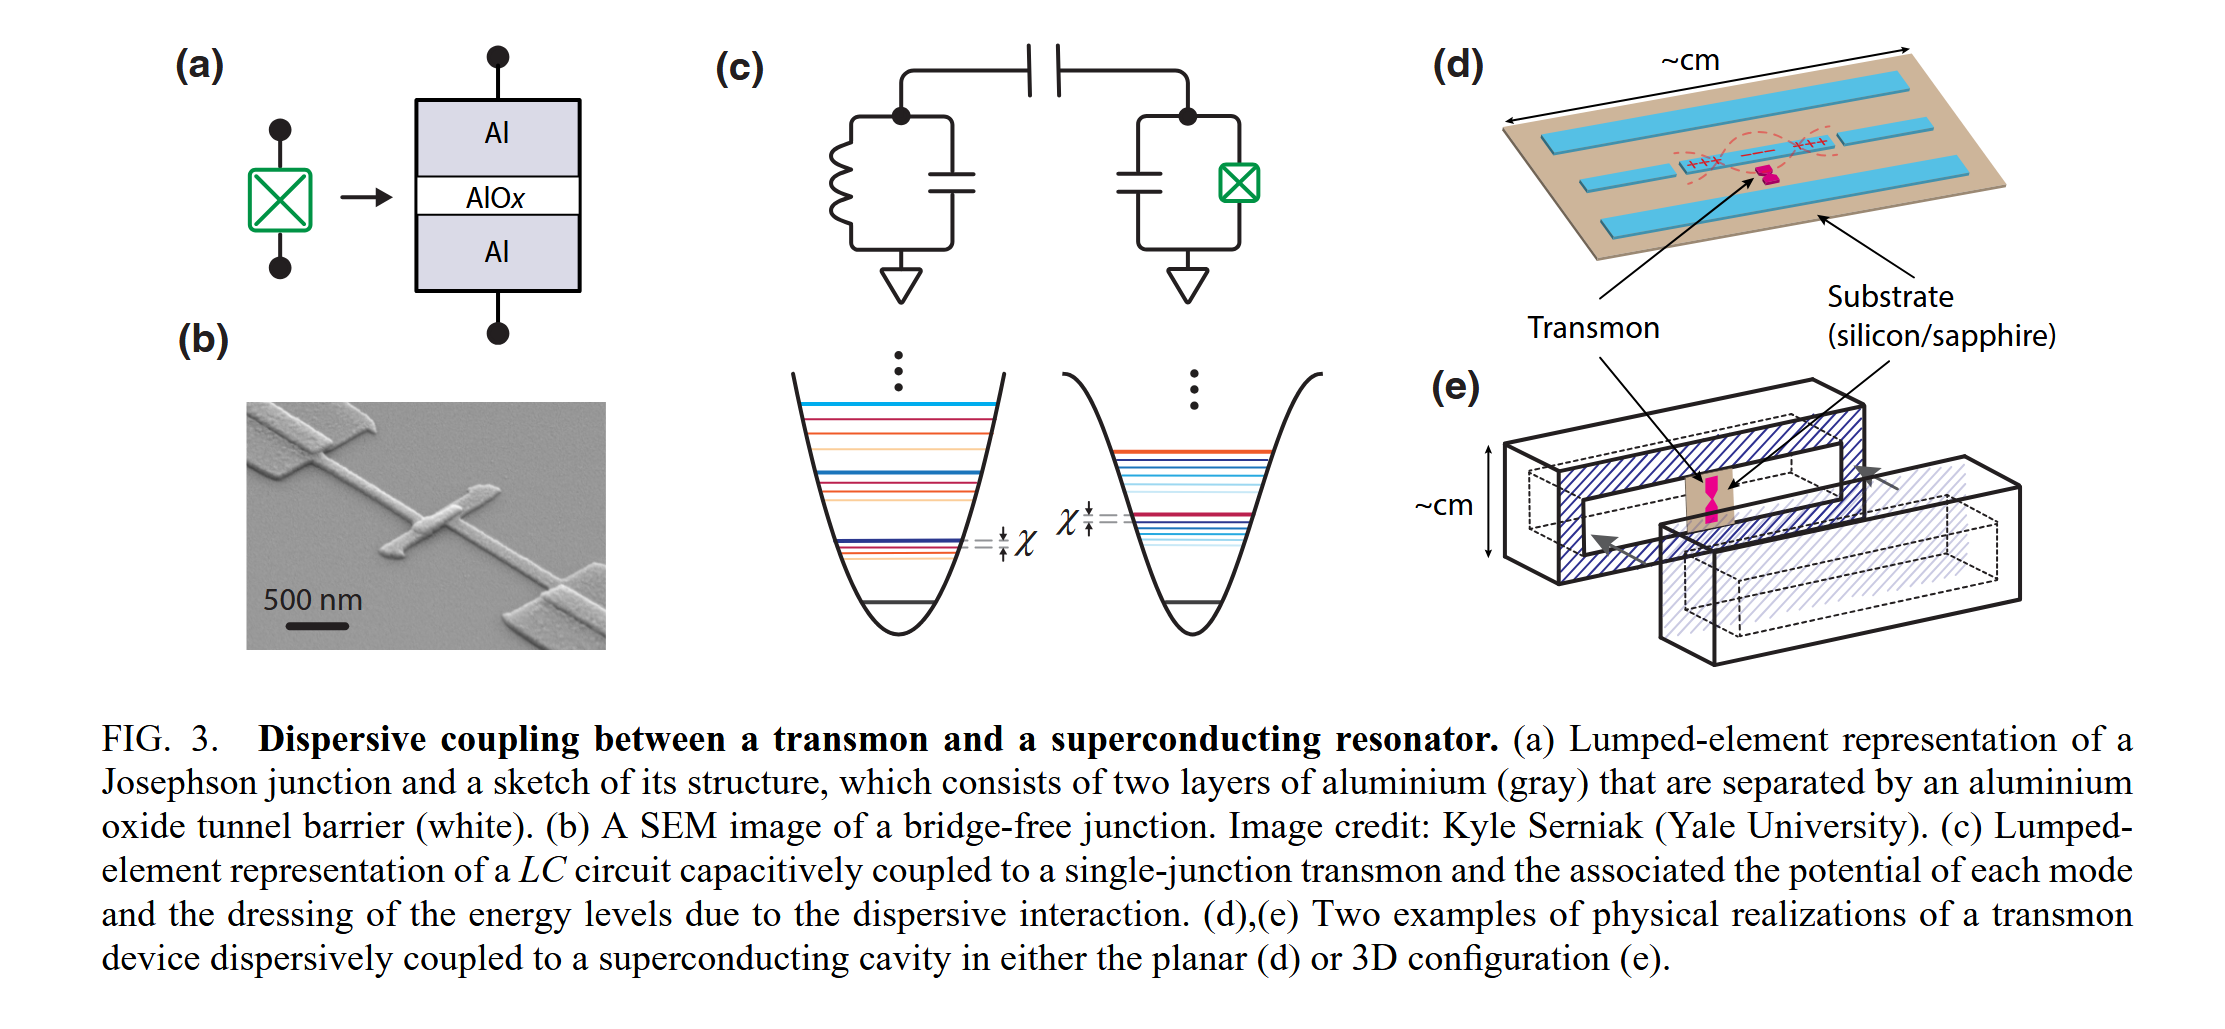
\includegraphics[width=0.9\textwidth]{img/couple.png}
    \caption{Transmon 与超导谐振器之间的色散耦合及其物理实现。}
    \label{fig:3}
\end{figure}

图 3 展示了 Transmon 与超导谐振器之间的色散耦合及其物理实现：
\begin{itemize}[leftmargin=2em]
    \item 图 3(a)：约瑟夫森结的集总元件表示，以及其由两层铝和一层氧化铝隧穿势垒组成的结构示意；
    \item 图 3(b)：bridge-free 结的 SEM 图；
    \item 图 3(c)：一个 LC 电路通过电容耦合到单结 Transmon 的集总模型，同时示意了各模式的势阱以及色散相互作用导致的能级 dressing；
    \item 图 3(d)、3(e)：分别给出平面结构和三维腔结构中，Transmon 与超导腔/谐振器色散耦合的实现方式。
\end{itemize}

\paragraph{3. 常用参数区间与近似条件}

虽然关于含有上述耦合项的哈密顿量的严格对角化可以在多篇综述中找到 [37,38,41]，但这里关注 cQED 中最常见的参数区间，并给出其近似对角化。设失谐为
\[
    \Delta\equiv \omega_T-\omega_R.
\]
我们考虑以下条件同时成立的情形：

\begin{enumerate}[leftmargin=2em]
    \item
    \[
        g\ll |\Delta|=|\omega_T-\omega_R|,
    \]
    即量子比特与腔模\textbf{大失谐}。这使两者之间表现为\textbf{色散相互作用}，而不是共振能量交换。

    \item
    \[
        \frac{E_C}{\hbar}\ll |\Delta|,
    \]
    即 Transmon 的非简谐性较弱。

    \item
    \[
        |\Delta|\ll \omega_T+\omega_R,
    \]
    因而\textbf{反旋转项}可以忽略。
\end{enumerate}

在这个参数区间内，对式 (22) 应用 RWA，可将相互作用哈密顿量化简为
\[
    \frac{H_{\mathrm{int}}}{\hbar}
    =
    g(aq^\dagger+a^\dagger q).
\]

\paragraph{4. 海森堡图像下的 Langevin 方程}

于是，在海森堡图像中，\(a\) 和 \(q\) 满足以下方程：
\begin{equation}
    \partial_t a
    =
    -i\left(\omega_R-i\frac{\kappa}{2}\right)a
    -igq,
    \tag{23}
\end{equation}
\begin{equation}
    \partial_t q
    =
    -i\omega_T q
    -iga
    -\frac{i}{\hbar}
    \left[
        q,
        H_{4+}\!\left(\varphi_T^{\mathrm{ZPF}}(q+q^\dagger)\right)
    \right].
    \tag{24}
\end{equation}

这里：
\begin{itemize}[leftmargin=2em]
    \item 我们只保留了谐振器的耗散；
    \item 忽略了 Transmon 的耗散；
    \item 这样做是为了分析读出腔（通常 \(Q\) 值较低或中等）对 Transmon 弛豫过程的影响。
\end{itemize}

\paragraph{5. 线性部分的对角化与 Lamb 位移}

将式 (24) 中的非线性部分视为微扰，先对线性部分进行对角化，其对应矩阵为
\begin{equation}
    M=
    \begin{pmatrix}
        \omega_R-i\kappa/2 & g\\
        g & \omega_T
    \end{pmatrix}.
    \tag{25}
\end{equation}

其本征值在一阶近似下为
\begin{equation}
    \tilde\omega_R
    =
    \omega_R+\frac{g^2}{\Delta}
    -i\frac{\kappa}{2}
    +i\left(\frac{g}{\Delta}\right)^2\frac{\kappa}{2},
    \tag{26}
\end{equation}
\begin{equation}
    \tilde\omega_T
    =
    \omega_T-\frac{g^2}{\Delta}
    -i\left(\frac{g}{\Delta}\right)^2\frac{\kappa}{2}.
    \tag{27}
\end{equation}

因此，相对于未耦合系统，色散耦合导致谐振器和 Transmon 的频率发生偏移，这一偏移就是\textbf{Lamb 位移}：
\begin{equation}
    \Delta_\chi=\frac{g^2}{\Delta}.
    \tag{28}
\end{equation}

\paragraph{6. Purcell 效应}

此外，Transmon 还会继承来自腔的部分耗散，其衰减速率为
\begin{equation}
    \Gamma_P=\left(\frac{g}{\Delta}\right)^2\kappa.
    \tag{29}
\end{equation}
这就是\textbf{Purcell 速率}。

Purcell 效应意味着系统中存在一个重要折中：
\begin{itemize}[leftmargin=2em]
    \item 较大的 Transmon--谐振器耦合强度有利于更快操作；
    \item 但同时可能缩短量子比特寿命。
\end{itemize}

不过在实际器件中，Purcell 效应可以借助精心设计的 \textbf{Purcell filter} 被显著抑制 [59]。

\paragraph{7. Dressed 模与混合角}

接下来定义一组新的湮灭与产生算符，它们对应矩阵 \(M\) 的本征向量。先引入混合角
\[
    \theta=\frac{1}{2}\arctan\!\left(\frac{2g}{\Delta}\right).
\]
则新的本征模（也称 \textbf{dressed modes}）为
\begin{equation}
    \tilde a
    =
    \cos(\theta)a+\sin(\theta)q
    \approx
    a+\frac{g}{\Delta}q,
    \tag{30}
\end{equation}
\begin{equation}
    \tilde q
    =
    -\sin(\theta)a+\cos(\theta)q
    \approx
    -\frac{g}{\Delta}a+q.
    \tag{31}
\end{equation}

\paragraph{8. 将 Transmon 非线性投影到 dressed 模上}

利用上式，可以把非线性哈密顿量中的变量重新表示为
\[
    \varphi_T^{\mathrm{ZPF}}(q+q^\dagger)
    =
    \varphi_T^{\mathrm{ZPF}}
    \big[
        \cos(\theta)(\tilde q+\tilde q^\dagger)
        +
        \sin(\theta)(\tilde a+\tilde a^\dagger)
    \big].
\]
在小混合角极限下，
\begin{equation}
    \varphi_T^{\mathrm{ZPF}}(q+q^\dagger)
    \approx
    \varphi_T^{\mathrm{ZPF}}(\tilde q+\tilde q^\dagger)
    +
    \varphi_T^{\mathrm{ZPF}}\frac{g}{\Delta}(\tilde a+\tilde a^\dagger).
    \tag{32}
\end{equation}

实际处理中，常将零点涨落系数与混合角合并记为新的系数，例如：
\[
    \varphi_q=\varphi_T^{\mathrm{ZPF}}\cos\theta,
    \qquad
    \varphi_R=\varphi_T^{\mathrm{ZPF}}\sin\theta,
\]
分别用于描述 \((q+q^\dagger)\) 与 \((a+a^\dagger)\) 项。这一记号在 cQED 的 Transmon--腔系统处理中非常常见。

\paragraph{9. 有效色散哈密顿量}

由于
\[
    \varphi_T^{\mathrm{ZPF}}\ll 1,
\]
非线性哈密顿量中最主要的是\textbf{四阶项}。然后再做一次与式 (15) 到式 (17) 相同的 RWA，去掉非共振项，并在新参考系下省略波浪号，即得到色散区内的有效哈密顿量
\begin{equation}
    \frac{H}{\hbar}
    =
    \omega_T q^\dagger q
    +
    \omega_R a^\dagger a
    -
    \frac{\alpha}{2}q^{\dagger 2}q^2
    -
    \frac{K}{2}a^{\dagger 2}a^2
    -
    \chi\,(q^\dagger q)(a^\dagger a),
    \tag{33}
\end{equation}
其中
\begin{equation}
    K
    =
    \frac{E_J}{2\hbar}
    \left(\varphi_T^{\mathrm{ZPF}}\right)^4
    \left(\frac{g}{\Delta}\right)^4
    =
    \frac{E_C}{\hbar}\left(\frac{g}{\Delta}\right)^4,
    \tag{34}
\end{equation}
\begin{equation}
    \chi
    =
    \frac{E_J}{2\hbar}
    \left(\varphi_T^{\mathrm{ZPF}}\right)^4
    \left(\frac{g}{\Delta}\right)^2
    =
    2\frac{E_C}{\hbar}\left(\frac{g}{\Delta}\right)^2.
    \tag{35}
\end{equation}

其中：
\begin{itemize}[leftmargin=2em]
    \item \(K\) 被称为谐振器的\textbf{自 Kerr 非线性（self-Kerr）}；
    \item \(\chi\) 被称为谐振器与 Transmon 之间的\textbf{交叉 Kerr 非线性（cross-Kerr）}。
\end{itemize}

\paragraph{10. 色散耦合的物理解释与强色散区}

色散耦合最核心的物理含义是：\textbf{两个模式之间存在状态依赖的频率偏移}。也就是说，一个模式处于什么状态，会导致另一个模式的频率发生可观测的变化。

如果这种状态相关频移大于谐振器的线宽，则通常说系统处于\textbf{强色散区}。

\paragraph{11. 实际实现方式与 cQED 中的三项核心能力}

在实验中，这类色散耦合的 Transmon--谐振器系统可以通过让两者空间上接近，使其电磁场重叠来实现，如图 3(d) 与图 3(e) 所示。更详细的版图与器件结构将在原文后续章节（Sec. III）讨论。

尽管有效色散哈密顿量形式相对简单，它却是 cQED 中大量关键现象与操作的基础。总体而言，谐振器--Transmon 系统提供了三项核心能力：
\begin{enumerate}[leftmargin=2em]
    \item 若谐振器与传输线强耦合，可以对 Transmon 进行\textbf{快速而高效的读出}；
    \item 两个 Transmon 可以通过一个中介谐振器模式发生相互作用，谐振器因此可充当\textbf{量子总线（quantum bus）}，用于实现量子逻辑操作；
    \item Transmon 可作为一个\textbf{非线性辅助模（nonlinear ancilla）}，对谐振器态实施通用控制。
\end{enumerate}

\paragraph{12. 受驱动相互作用、四波混频与应用}

除了系统天然存在的相互作用外，在精心选择频率的微波驱动作用下，还可以进一步\textbf{工程化新的动力学}。这一能力来源于 JJ 中的\textbf{非线性频率混频}，其作用类似于非线性光学介质中的频率变换过程 [72]。在一阶近似下，单个 JJ 就可以在 cQED 器件中实现\textbf{四波混频}。

这类受驱动相互作用是设计新型动力学和量子操作的重要工具。一个关键应用是构建\textbf{量子极限放大器}，原文在 Sec. IV 中将进一步讨论。

此外，借助这种驱动工程，人们已经在实验中实现了种类丰富的有效哈密顿量，并推动了大量新进展，包括：
\begin{itemize}[leftmargin=2em]
    \item 薛定谔猫态的稳定与保护 [63,73--75]；
    \item 超导量子比特的远程纠缠 [76--79]；
    \item 纳米机械器件冷却 [80]；
    \item 微波腔之间的工程化量子门 [81--83]；
    \item 单个微波光子的探测 [84]；
    \item 腔与 Transmon 之间的纵向耦合 [15]；
    \item 以及更多基于 cQED 的新型实验方案。
\end{itemize}

\paragraph{13. 本节主线总结}

本节从 cQED 的两大基础元件出发，建立了如下完整逻辑：
\begin{itemize}[leftmargin=2em]
    \item 超导谐振器提供高相干的量子简谐模式；
    \item 约瑟夫森结提供简单而无耗散的非线性来源；
    \item Transmon 是在 \(E_J\gg E_C\) 区间工作的弱非简谐量子比特，兼顾低电荷噪声敏感性与足够的非简谐性；
    \item 当 Transmon 与谐振器在大失谐条件下耦合时，会形成色散耦合，其核心效应是状态依赖频移；
    \item 这一平台进一步支持高保真读出、量子总线、非线性控制与驱动工程，构成现代 cQED 与超导量子信息处理的核心物理基础。
\end{itemize}


\section{量子电路设计：从目标哈密顿量到物理实现}

\subsection{总体目标与设计闭环}

在电路量子电动力学（cQED）实验中，一旦针对某个应用已经确定了理想的目标哈密顿量，接下来的首要任务就是把一组抽象的系统参数转化为实际可制造的物理器件。这些抽象参数包括：
\begin{itemize}
    \item 量子比特数目；
    \item 跃迁频率；
    \item 各模之间的连通关系（connectivity）；
    \item 耦合强度；
    \item 相干性与退相干要求；
    \item 可调谐性、读出方式、控制方式等。
\end{itemize}

这一“从目标哈密顿量到物理器件”的转换并不是一次完成的，而是一个\textbf{迭代式设计流程}。其核心思想可以概括为：

\begin{enumerate}
    \item 从\textbf{目标哈密顿量}出发，明确理想系统需要哪些自由度与参数；
    \item 提出器件的\textbf{连通性要求}与\textbf{相干性要求}；
    \item 选择合适的\textbf{器件架构}（如平面架构或 3D 架构），并完成初步\textbf{器件布局}；
    \item 对构件进行\textbf{配置与重配置}，决定量子比特、谐振器、耦合器、读出端口等的具体形式；
    \item 进行\textbf{电磁仿真}（electromagnetic simulation），可靠求出器件的电磁本征模结构；
    \item 通过\textbf{电路量子化}与\textbf{参与比分析}等方法，从仿真中提取哈密顿量参数；
    \item 结合\textbf{退相干估计}，判断设计是否满足目标；
    \item 若不满足，则回到布局、参数或耦合设计阶段继续迭代；
    \item 当物理实现与目标哈密顿量充分一致时，再进入\textbf{制备（fabrication）}阶段。
\end{enumerate}

这一流程的关键点在于：\textbf{“理想目标”与“物理实现”之间通过仿真、量子化和退相干评估不断闭环校正}。因此，量子电路设计本质上是一个多目标折中问题：既要满足所需哈密顿量，又要兼顾可制造性、可控制性和相干性。

\subsection{器件架构：平面架构与 3D 架构}

\subsubsection{两类主流架构的基本区分}

目前 cQED 中主流的器件架构大致分为两类：

\begin{itemize}
    \item \textbf{平面（planar）架构}：所有量子模（例如量子比特、线性谐振器）都通过芯片上的光刻图形定义；
    \item \textbf{3D 架构}：部分量子模原生存在于三维腔体等三维结构中。
\end{itemize}

尽管这两类架构差异很大，但二者有一个共同点：都需要一个经过工程化设计的\textbf{三维封装（sample box）}，用来约束器件的电磁模，并抑制由微波辐射损耗引发的退相干。

\subsubsection{3D 架构}

在 3D 架构中，封装内部较大的真空体积本身就可以作为 cQED 哈密顿量中的\textbf{线性模}。典型 3D 腔体体积可达几个 \(\mathrm{cm}^3\)。

\paragraph{基本物理实现}
3D 架构中的几个核心特征如下：
\begin{itemize}
    \item 大体积的 3D 腔体模式充当线性谐振模；
    \item 腔体通过\textbf{同轴电缆中心针}穿过腔壁上的孔与传输线弱耦合；
    \item 腔体还会与量子比特或其他谐振模耦合；
    \item 这些量子比特/附加谐振器通常仍通过\textbf{光刻平面结构}实现，并设计较大的电容焊盘，以增强与 3D 腔模的耦合；
    \item 芯片可以制作在一个或多个芯片上，并通过机械夹紧、螺钉、螺母等方式固定在腔体内部。
\end{itemize}

\paragraph{典型器件构成（对应图 5）}
\begin{figure}[htbp]
    \centering
    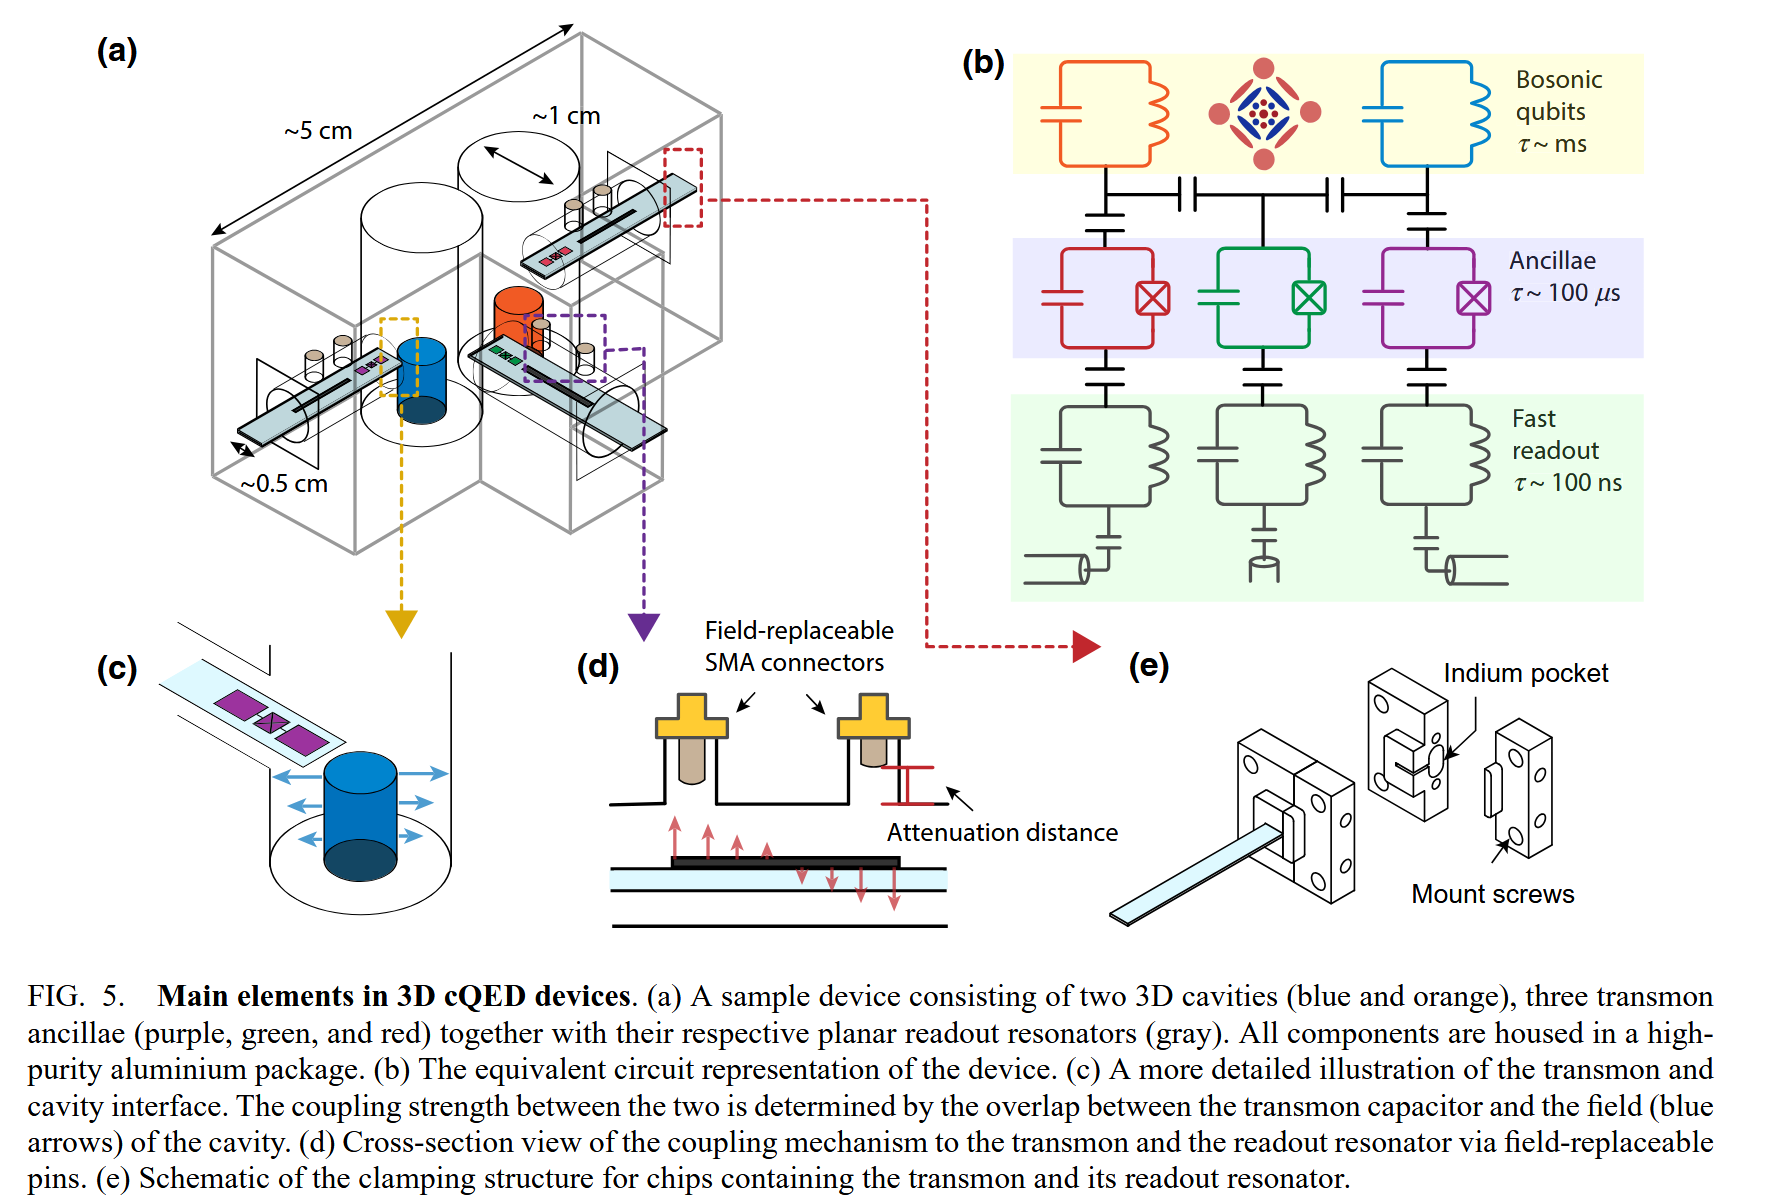
\includegraphics[width=0.9\textwidth]{img/3D cQED.png}
    \caption{3D cQED 器件的典型构成与电路模型。}
    \label{fig:5}
\end{figure}
一个代表性的 3D cQED 器件可以包括：
\begin{itemize}
    \item 两个 3D 腔体（可作为玻色编码量子存储）；
    \item 三个 transmon 辅助量子比特（ancillae）；
    \item 每个辅助量子比特对应一个平面读出谐振器；
    \item 所有组件被封装在高纯铝腔体中。
\end{itemize}

从等效电路角度看，这类器件往往同时包含不同时间尺度的模：
\begin{itemize}
    \item \textbf{玻色量子比特/长寿命腔模}：寿命可达毫秒量级；
    \item \textbf{辅助 transmon}：相干时间常在 \(100~\mu\mathrm{s}\) 量级；
    \item \textbf{快速读出模}：时间尺度可短至 \(100~\mathrm{ns}\) 量级。
\end{itemize}

腔体与 transmon 的耦合强度主要取决于\textbf{transmon 电容焊盘与腔体电场分布的重叠程度}。而读出与外部线缆的耦合，则常通过可更换的同轴针结构调节。

\paragraph{3D 架构的优点}
对于小规模量子电路，尤其是初学者实验平台，3D 架构有以下优势：
\begin{enumerate}
    \item \textbf{装配简单}：不需要额外的 PCB、线键合（wire bonds）等外围结构去桥接量子模与外部线缆；
    \item \textbf{电磁环境更干净}：外围结构减少后，封装中杂散模的抑制更容易；
    \item \textbf{相干性通常更好}：在相同材料品质下，由于量子模的表面积/体积比较小，表面损耗通常更低；尤其是长寿命 3D 腔模，常可作为优质量子存储资源。
\end{enumerate}

因此，3D cQED 器件是量子纠错与玻色量子模拟的重要实验平台。

\paragraph{3D 架构的局限}
目前基于机加工腔体的 3D 器件仍存在一些重要限制：
\begin{itemize}
    \item \textbf{模隔离困难}：3D 腔体电磁场空间范围较大，因此在同一腔体内实现良好的模隔离并不容易；
    \item \textbf{直流连接不足}：芯片缺少方便的 dc 连接，不利于需要磁通偏置的可调谐元件；
    \item \textbf{可扩展性挑战}：复杂布线、局域快速磁通控制等功能在 3D 环境中仍在持续发展中。
\end{itemize}

\subsubsection{平面架构}

平面架构以\textbf{光刻定义的超导芯片}为中心。芯片本身定义了应用所需的大部分量子模，尽管外部封装仍会影响哈密顿量参数的细节。

\paragraph{基本物理实现}
平面 cQED 芯片除量子电路元件外，通常还集成：
\begin{itemize}
    \item \textbf{馈线（feedlines）}；
    \item 这些馈线通常采用\textbf{共面波导（CPW）}形式，并与输入/输出同轴电缆做阻抗匹配；
    \item 馈线与量子电路元件弱耦合，用于注入和提取微波信号。
\end{itemize}

封装层面，一般采用如下结构：
\begin{itemize}
    \item 芯片嵌入 PCB；
    \item 芯片 CPW 端口与 PCB 上相应端口连接；
    \item 芯片接地面与 PCB 接地面常通过大量 wire bonds 连接；
    \item PCB 上加装块状超导盖板，将芯片围入尽可能小的体积中，以抑制 box modes；
    \item 在没有片上三维互连的情况下，这种封装区域通常被限制在约 \(1~\mathrm{cm}^2\) 以内；
    \item PCB 再把输入输出信号引到平面--同轴过渡结构，与外部线缆相连。
\end{itemize}

\paragraph{典型器件构成（对应图 6）}
\begin{figure}[htbp]
    \centering
    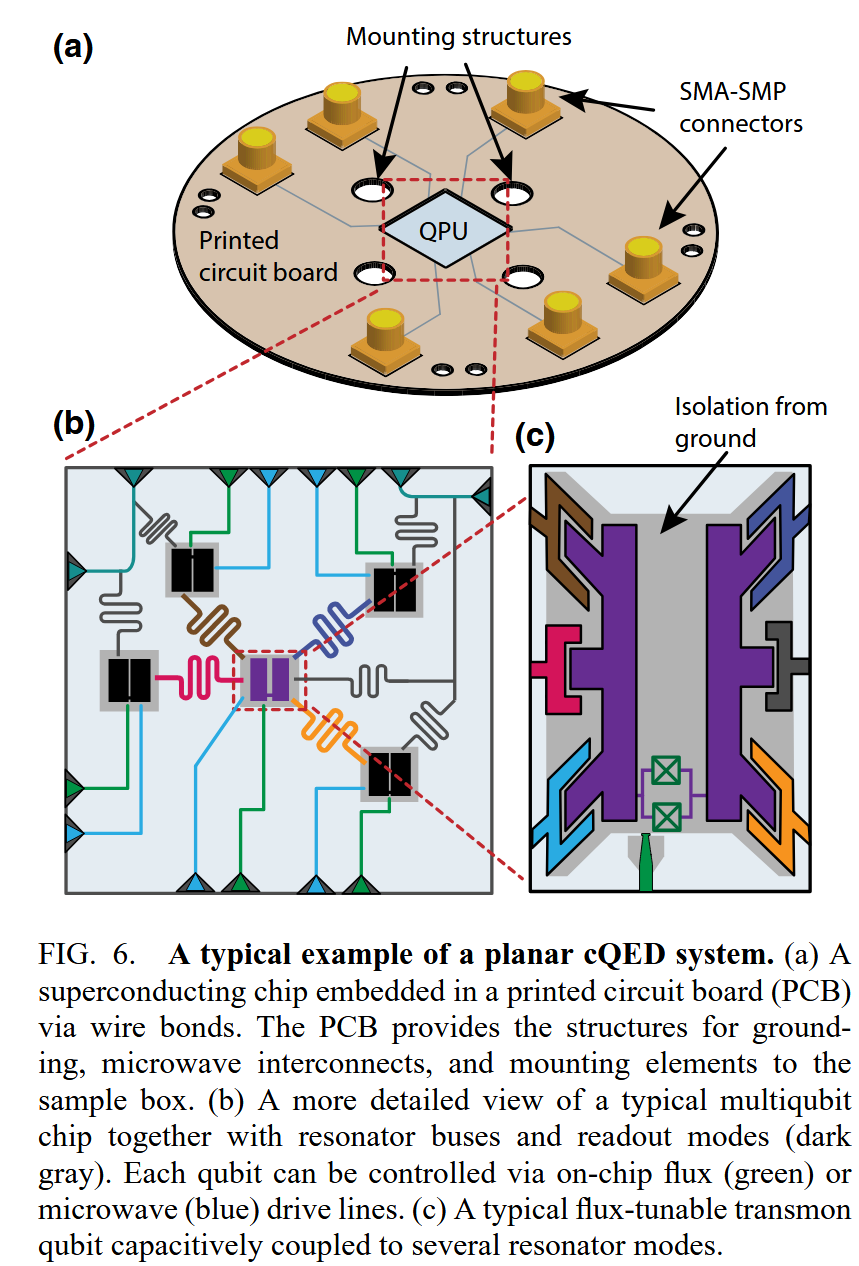
\includegraphics[width=0.9\textwidth]{img/planar cQED.png}
    \caption{平面 cQED 器件的典型构成与电路模型。}
    \label{fig:6}
\end{figure}
典型的平面 cQED 系统包含：
\begin{itemize}
    \item 嵌入 PCB 的超导芯片；
    \item 多个量子比特；
    \item 总线谐振器与读出谐振器；
    \item 片上磁通控制线（绿色）与微波驱动线（蓝色）；
    \item 通过电容耦合到多个谐振器模的可调谐 transmon。
\end{itemize}

\paragraph{平面架构的优势}
由于电磁模与耦合结构更加局域化，经过良好工程设计的平面 cQED 器件具有以下优点：
\begin{enumerate}
    \item \textbf{快速磁通控制}：便于对量子比特、谐振器或耦合元件进行快速磁通调制；
    \item \textbf{多元件独立设计}：在同一芯片上可设计大量量子元件，并保持参数之间较低的交叉依赖；
    \item \textbf{局域访问灵活}：可以较方便地对单个元件施加局域控制与读出。
\end{enumerate}

因此，近期包含十多个量子比特和谐振器的实验，大多采用平面方案。

\paragraph{平面架构的扩展挑战与未来趋势}
当器件规模进一步扩展到 \(50\) 个量子比特以上时，仅靠传统平面方法可能不够，往往需要引入：
\begin{itemize}
    \item 翻转芯片铟键合（flip-chip indium bonding）；
    \item 硅通孔（through-silicon vias, TSV）；
    \item 其他片上 3D 集成技术。
\end{itemize}

从长期看，平面与 3D 两类架构虽然目前在 box modes 与接地平面的处理方式上差异显著，但未来很可能在技术平台上逐渐趋同。

\subsection{构建基本模块：从需求到具体电路}

\subsubsection{设计起点：先回答哪些问题}

在真正开始画器件之前，首先需要回答如下基本问题：
\begin{itemize}
    \item 需要多少个\textbf{非线性元件}（如量子比特）？
    \item 需要多少个\textbf{线性元件}（如谐振器）？
    \item 每个元件分别承担什么功能？其目标频率是多少？
    \item 是否需要可调谐性？需要怎样的控制端口？
    \item 对每个元件的相干时间要求是什么？
    \item 各元件之间需要怎样的连接关系？
    \item 它们是通过电容耦合、感应耦合，还是通过中介模耦合？
\end{itemize}

这些问题往往会直接决定：当前技术条件下应优先选择平面方案还是 3D 方案。

\subsubsection{线性模：谐振器的实现}

无论是平面还是 3D cQED，线性模通常由\textbf{超导谐振器}实现，其频率主要由电磁结构的几何尺寸决定。

\paragraph{通用认识}
\begin{itemize}
    \item 集总参数 \(LC\) 谐振器（如叉指电容加蛇形电感）适合小尺寸设计；
    \item 但在实际 cQED 中，最常见的仍是：
    \begin{itemize}
        \item 平面中的 \textbf{CPW 谐振器}；
        \item 3D 方案中的\textbf{同轴谐振器变体}。
    \end{itemize}
    \item 从物理上看，它们都可以理解为\textbf{无限级联的 \(LC\) 振子链}；
    \item 实验中通常只使用\textbf{基模}，但高阶模依然存在；
    \item 因此必须保证高阶模与目标频率充分失谐，以免影响器件工作；
    \item 高阶模还可能导致热光子散粒噪声退相干、以及杂散多光子跃迁等问题。
\end{itemize}

\paragraph{CPW 谐振器}
CPW 谐振器本质上是两端满足特定边界条件的 CPW 传输线段。

其关键参数包括：
\begin{itemize}
    \item 单位长度几何电容 \(C_g\)；
    \item 单位长度几何电感 \(L_g\)；
    \item 超导薄膜的单位长度动能电感 \(L_k\)。
\end{itemize}

其中：
\begin{itemize}
    \item \(C_g\) 与 \(L_g\) 由 CPW 截面几何决定，例如中心导体宽度和缝隙宽度；
    \item \(L_k\) 与材料参数和几何尺寸有关，可由薄膜室温电阻率等估计；
    \item 在标准平面器件中，\(L_k\) 的贡献通常较小，但不能完全忽略。
\end{itemize}

传播波长由这些参数共同决定，可写为
\[
\lambda = \frac{2\pi}{\omega\sqrt{C_g\,(L_g+L_k)}}.
\]

据此：
\begin{itemize}
    \item 双开路端形成 \(\lambda/2\) 谐振器；
    \item 一端开路、一端短路形成 \(\lambda/4\) 谐振器。
\end{itemize}

典型地，工作频率约 \(5~\mathrm{GHz}\) 时，对应的 CPW 长度约为厘米量级；但可以通过蛇形（meandering）走线显著缩小实际占地面积。

\paragraph{同轴/3D 谐振器}
同轴谐振器同样可以理解为满足不同边界条件的同轴传输线段。

两种重要形式为：
\begin{itemize}
    \item \(\lambda/4\) 同轴谐振器：可通过整块体超导材料机加工而成，从而避免金属装配接缝引起的欧姆损耗；
    \item \(\lambda/2\) 同轴谐振器：常采用机加工金属管作为接地屏蔽，内部悬置超导条带作为中心导体。
\end{itemize}

其中：
\begin{itemize}
    \item 前者对应“reentrant post-cavity”类型，常能获得极高相干性，是高 \(Q\) 量子存储的有力方案；
    \item 后者则更适合在同一芯片上集成多个谐振器、量子比特与 Purcell filter，并通过主要由光刻定义的耦合方式进行系统级设计。
\end{itemize}

所需谐振器长度同样可由目标频率下的传播波长估算。

\subsubsection{非线性模：量子比特、耦合器与参量器件}

非线性模（例如量子比特、耦合器、参量混频器）的设计通常从\textbf{集总参数近似}开始。

\paragraph{基本构成}
\begin{itemize}
    \item 电感部分由\textbf{约瑟夫森结（JJ）}提供；
    \item 其非线性电感可通过调节隧穿结面积方便地改变；
    \item 电容则通过改变超导引线和焊盘尺寸来调节。
\end{itemize}

\paragraph{以 transmon 为例的典型设计范围}
对于 transmon 量子比特，目标频率通常在 \(4\) 到 \(8~\mathrm{GHz}\) 之间。选择这一范围的原因有三：
\begin{enumerate}
    \item 在 \(20~\mathrm{mK}\) 左右的温度下足够高，可抑制热激发；
    \item 又不会高到显著增强与更高频杂散封装模的耦合；
    \item 同时适配现有高性能且成本相对可控的微波电子学。
\end{enumerate}

典型参数范围为：
\begin{itemize}
    \item 电感：\(6\) 到 \(16~\mathrm{nH}\)；
    \item 电容：\(50\) 到 \(125~\mathrm{fF}\)；
    \item 其中结隧穿势垒本身常贡献 \(2\) 到 \(5~\mathrm{fF}\) 电容；
    \item 对应 \(E_J/h \sim 10\) 到 \(25~\mathrm{GHz}\)；
    \item 对应 \(E_C/h \sim 160\) 到 \(400~\mathrm{MHz}\)。
\end{itemize}

选取这样的 \(E_C\) 范围，是为了在\textbf{抑制电荷噪声}与\textbf{保持足够非简谐性}之间做平衡。对于 transmon，非简谐性通常近似满足
\[
\alpha \approx E_C/h,
\]
而足够的非简谐性对快速量子门操作十分重要。

\subsubsection{耦合设计与频率布局}

器件中不同模之间的耦合设计是实现目标哈密顿量的核心。

\paragraph{电容耦合与感应耦合}
以 transmon 与谐振器为例，其色散耦合可以通过增大两者电磁场重叠来实现。等价地说：
\begin{itemize}
    \item 若两模之间互电容较大，则容易获得较强的耦合强度 \(g\)；
    \item 也可通过互感实现感应耦合。
\end{itemize}

在平面设计中，耦合电容常由特定几何结构（如叉形电容耦合结构）形成，其数值可借助：
\begin{itemize}
    \item 保角映射方法；
    \item 针对特定几何的解析近似公式；
    \item 或更精确的全波仿真。
\end{itemize}

\paragraph{耦合不仅取决于 \(g\)，也取决于失谐}
色散相互作用强度 \(\chi\) 不仅依赖耦合强度 \(g\)，还依赖元件之间的频率失谐 \(\Delta\)。因此，除了设计耦合元件本身之外，也可通过修改各元件尺寸来改变其本征频率，从而调节 \(\chi\)。

\paragraph{多量子比特系统中的频率规划}
如果目标哈密顿量需要多个量子比特及其门操作，则几何布局应满足：
\begin{itemize}
    \item 相关共振频率彼此适当分离；
    \item 无关模之间的互电容/互感尽量小；
    \item 尽量避免非目标耦合与串扰。
\end{itemize}

\subsubsection{元件功能定位：读出、存储、总线与控制}

\paragraph{谐振器的三类典型功能}
谐振器在 cQED 中通常承担三类功能：
\begin{enumerate}
    \item \textbf{读出谐振器（readout resonator）}；
    \item \textbf{存储谐振器（memory resonator）}；
    \item \textbf{总线谐振器（bus resonator）}。
\end{enumerate}

对于读出谐振器，应较强地耦合到传输线，以便高效提取信息。其输出耦合品质因数 \(Q\) 通常设计在
\[
10^3 \sim 10^4
\]
量级。

不同架构中，读出耦合的控制方式也不同：
\begin{itemize}
    \item 在平面设计中，CPW 谐振器与馈线之间的耦合 \(Q\) 常由谐振器末端的\textbf{耦合电容}控制；
    \item 在 3D 设计中，腔体与外部传输线的耦合 \(Q\) 常由插入腔壁中的\textbf{耦合针长度}控制。
\end{itemize}

而对于长寿命量子存储谐振器，则应使其输入耦合 \(Q\) 足够高，以免外部驱动线显著降低总品质因数。

\paragraph{量子比特的功能与可调谐性}
不同功能需求会对应不同量子比特结构：
\begin{itemize}
    \item \textbf{固定频率 transmon}：通常只需一个 JJ 连接两个超导焊盘；
    \item \textbf{磁通可调量子比特}：需要更多 JJ 形成磁通回路。
\end{itemize}

常见可调谐结构包括：
\begin{itemize}
    \item 对称 SQUID transmon；
    \item 非对称 SQUID transmon；
    \item SNAIL；
    \item flux qubit；
    \item fluxonium。
\end{itemize}

一旦引入磁通可调元件，就必须进一步设计\textbf{磁通偏置线}：
\begin{itemize}
    \item 在平面器件中，常使用靠近磁通环的短路端 CPW 作为偏置线；
    \item 在 3D 架构中，目前可使用厘米尺度的外部线圈，为铜封装内的可调器件提供\textbf{全局直流磁通}；
    \item 但\textbf{快速、局域}的磁通偏置在 3D 架构中仍是发展中的技术。
\end{itemize}

\paragraph{微波控制线}
控制这些量子元件还需要精心设计的微波馈线：
\begin{itemize}
    \item 对固定频率 transmon，需要通过\textbf{电容耦合驱动线}实现 \(X/Y\) 控制；
    \item 对磁通可调器件，则还需要\textbf{感应耦合的磁通偏置线}。
\end{itemize}

但是，这些额外的控制结构都会把量子系统更强地暴露在耗散环境中，从而可能降低器件的相干时间。

\subsubsection{控制线路引入的耗散与相干性代价}

附加的驱动线与偏置线会给量子比特引入额外弛豫通道。可用一个包含耗散环境阻抗 \(\mathrm{Re}[Z(\omega)]\) 的电路模型来估算弛豫率：

\begin{equation}
\Gamma = \frac{1}{\mathrm{Re}[Z(\omega)]\,C_{\Sigma}},
\tag{36}
\end{equation}
其中 \(C_{\Sigma}\) 是 transmon 的有效总电容。

\paragraph{微波驱动线引起的衰减}
若 transmon 通过电容 \(C_c\) 与一条微波驱动线耦合，则其有效衰减率近似为
\begin{equation}
\Gamma_D \simeq \omega_q^2 Z_0 \frac{C_c^2}{C_{\Sigma}},
\tag{37}
\end{equation}
其中：
\begin{itemize}
    \item \(\omega_q\) 为量子比特共振频率；
    \item \(Z_0\) 为特征阻抗，通常取 \(50~\Omega\)；
    \item \(C_c\) 为耦合电容。
\end{itemize}

若取典型参数
\[
\omega_q = 2\pi\times 5~\mathrm{GHz},\qquad
C_{\Sigma}=65~\mathrm{fF},\qquad
C_c=0.1~\mathrm{fF},
\]
则得到
\[
T_1 = \frac{1}{\Gamma_D} \approx 132~\mu\mathrm{s}.
\]

\paragraph{磁通偏置线引起的衰减}
若将磁通偏置线建模为与 transmon 串联的电容 \(C_c\) 和并联电感 \(L_c\)，则其有效衰减率为
\begin{equation}
\Gamma_{\mathrm{FBL}} \simeq \frac{1}{Z_0 C_{\Sigma}}
\left(\frac{\omega_q}{\omega_c}\right)^4,
\qquad
\omega_c = \frac{1}{\sqrt{L_c C_c}}.
\tag{38}
\end{equation}

若取
\[
\omega_q = 2\pi\times 5~\mathrm{GHz},\qquad
C_{\Sigma}=65~\mathrm{fF},\qquad
C_c=10~\mathrm{fF},\qquad
L_c=20~\mathrm{pH},
\]
则可得
\[
T_1 = \frac{1}{\Gamma_{\mathrm{FBL}}} \approx 83~\mu\mathrm{s}.
\]

\paragraph{理解这些公式时的注意事项}
\begin{itemize}
    \item 以上估算主要是\textbf{经验量级公式}；
    \item 实际超导量子器件通常比这些简化模型复杂得多；
    \item 因此在实际设计中，常借助如 \texttt{QuCAT}、\texttt{scqubits} 等软件，更准确计算器件参数与耗散率。
\end{itemize}

\subsection{电磁仿真与系统参数提取}

\subsubsection{为什么需要电磁仿真}

完成器件的初步布局之后，需要通过数值仿真提取系统参数。常用的 GHz 频段电磁仿真软件包括：
\begin{itemize}
    \item Ansys HFSS；
    \item COMSOL；
    \item Sonnet。
\end{itemize}

这些求解器可以帮助我们：
\begin{itemize}
    \item 可视化器件中各个共振模的电磁场分布；
    \item 分析各模之间的耦合强度；
    \item 评估它们与外部环境的耦合；
    \item 为后续电路量子化提供输入数据。
\end{itemize}

\subsubsection{仿真中的建模近似}

在这类仿真中，约瑟夫森结通常被视为一个简单的\textbf{集总元件结构}，由以下两部分构成：
\begin{itemize}
    \item 一个电感；
    \item 一个较小的电容。
\end{itemize}

其中：
\begin{itemize}
    \item 这些参数来自结本身的工艺规格，而不是完全由电磁仿真自动给出；
    \item transmon 的绝大部分电感都来自结的动能电感；
    \item transmon 的其余金属结构与平面腔模通常近似为\textbf{理想导体金属片}，因为它们的动能电感相较于 JJ 很小；
    \item 对于 3D 腔体，则可将其建模为真空盒，其几何尺寸决定腔体的共振模。
\end{itemize}

\subsubsection{网格与收敛设置}

为了可靠捕捉器件中的共振模，网格与收敛标准必须谨慎设定。

\paragraph{网格策略}
\begin{itemize}
    \item 更细的表面网格可以更准确地评估电磁场分布；
    \item 但同时会显著增加计算代价；
    \item 因此通常采用\textbf{非均匀网格}：
    \begin{itemize}
        \item 在小尺寸结构、尖角、边缘等电场集中区域使用更细网格；
        \item 在大面积、规则、场分布较平缓的区域使用较粗网格。
    \end{itemize}
\end{itemize}

\paragraph{收敛标准}
\begin{itemize}
    \item 收敛标准的选择取决于仿真目标；
    \item 若目标是准确捕捉模频率，则常要求每次迭代的频率收敛误差达到 \(0.1\%\) 甚至更小。
\end{itemize}

\subsubsection{从仿真结果到哈密顿量参数}

在获得电磁仿真结果后，需要进一步把这些经典场信息转化为量子哈密顿量参数。文中强调了两种主要方法：

\paragraph{1.\ 黑箱量子化（BBQ, blackbox quantization）}
其核心思想是：
\begin{itemize}
    \item 把约瑟夫森结视为嵌入在线性电感--电容网络中的\textbf{小非线性微扰}；
    \item 通过分析电路阻抗中的零点与极点，提取相关哈密顿量参数；
    \item 该方法后来也被推广到包含多个非线性模的多模系统。
\end{itemize}

BBQ 的优点是：
\begin{itemize}
    \item 对 cQED 系统的关键哈密顿量参数提供了系统分析工具；
\end{itemize}

但其代价是：
\begin{itemize}
    \item 需要额外的仿真步骤来获得电路的数值阻抗信息。
\end{itemize}

\paragraph{2.\ 能量参与比（EPR, energy participation ratio）方法}
EPR 提供了一个更直接、通常也更简洁的替代方案。其基本思想是：
\begin{itemize}
    \item 直接利用有限元仿真得到的电磁场分布；
    \item 根据各个非线性元件在不同模式中“分担了多少电感能量”，提取哈密顿量参数。
\end{itemize}

对于模式 \(m\) 中的结元件 \(j\)，其参与比 \(p_{mj}\) 定义为该结中储存的电感能量占模式 \(m\) 总电感能量的比例，即
\[
p_{mj}=\frac{U^{(L)}_{mj}}{U^{(L)}_{m}},
\qquad 0\le p_{mj}\le 1.
\]

其物理意义为：
\begin{itemize}
    \item 若 \(p_{mj}=0\)，说明结 \(j\) 不参与模式 \(m\)；
    \item 若 \(p_{mj}=1\)，说明模式 \(m\) 的电感能量全部集中在该结上，即它是该模式唯一被激发的电感元件。
\end{itemize}

基于 \(p_{mj}\)，可以直接提取：
\begin{itemize}
    \item 模频率 \(\omega_i\)；
    \item 非线性耦合项 \(\chi_{ik}\)；
    \item 以及其他哈密顿量中的关键参数。
\end{itemize}

EPR 的优势在于：
\begin{itemize}
    \item 所需仿真次数更少；
    \item 对包含一个或多个非线性元件的复杂电路都具有较好的普适性；
    \item 近年来已被广泛采用，并且相关实现已开源。
\end{itemize}

\subsection{平面 cQED 器件中的潜在损耗通道}

除了频率与耦合设计，实际器件还必须面对损耗与噪声源。对于平面 cQED 器件，典型损耗通道包括：

\begin{itemize}
    \item 与外界的不期望耦合；
    \item 封装或结构中的杂散模；
    \item 材料本身的耗散；
    \item 辐射损耗。
\end{itemize}

在一个典型平面器件中：
\begin{itemize}
    \item 光刻芯片放置在电路板支架中；
    \item 支架再置于金属封装内部；
    \item 整个环境中的多种损耗都可以用等效电阻来表征。
\end{itemize}

\subsubsection{界面损耗是平面器件的重要问题}

图示中尤其强调了超导图形边缘截面的几类表面/界面损耗。常见三类界面为：
\begin{itemize}
    \item \textbf{MS}：金属--衬底（metal-substrate）界面；
    \item \textbf{MA}：金属--空气（metal-air）界面；
    \item \textbf{SA}：衬底--空气（substrate-air）界面。
\end{itemize}

此外，超导薄膜厚度 \(h\) 所对应的区域还可进一步分成：
\begin{itemize}
    \item \textbf{内部区域}；
    \item \textbf{边缘区域}。
\end{itemize}

这些区域对总损耗的贡献不同，且可以通过仿真进行量化比较。因此，在平面器件设计中，\textbf{材料界面工程、边缘几何与封装电磁环境}都会显著影响最终相干性。

\subsection{本部分内容的逻辑总结}

本部分的主线可以概括为：

\begin{enumerate}
    \item \textbf{先从目标哈密顿量出发}，明确所需模、频率、耦合和相干性；
    \item \textbf{再选择架构}：平面方案强调局域布线与可扩展控制，3D 方案强调干净电磁环境与高相干；
    \item \textbf{随后配置构件}：包括线性谐振器、非线性元件、耦合结构、读出接口与控制线；
    \item \textbf{接着评估代价}：尤其是额外控制线路带来的耗散与相干性下降；
    \item \textbf{最后通过电磁仿真与量子化}，把几何设计转化为哈密顿量参数，并通过 BBQ 或 EPR 等方法提取有效模型；
    \item \textbf{在整个过程中不断迭代}，直到物理器件与目标哈密顿量一致，并且满足相干性与实验可操作性要求。
\end{enumerate}

换言之，量子电路设计并不是简单“画一个电路”，而是一个贯穿\textbf{架构选择、模设计、耦合设计、控制设计、损耗分析、数值仿真与量子化提取}的系统工程。
\subsection{最优相干性的设计考量}

\subsubsection{退相干并不完全由电路参数决定}

虽然哈密顿量参数、输入输出耦合参数等往往可以通过电路设计较为准确地控制，但量子电路中的\textbf{退相干（decoherence）}却通常由器件与环境中大量自由度之间残余而微弱的相互作用所决定，而这些环境自由度并不都处于设计者的直接控制之下。

从噪声作用方向来看，这些相互作用大致可分为两类：
\begin{itemize}
    \item \textbf{横向噪声（transverse noise）}：相对于量子比特量子化轴为横向耦合，主要导致\textbf{能量弛豫}，即 \(T_1\) 过程；
    \item \textbf{纵向噪声（longitudinal noise）}：沿量子化轴耦合，主要导致\textbf{退相位}，即 \(T_\phi\) 过程。
\end{itemize}

对于平面 cQED 器件，前文图示已经给出了若干典型潜在损耗源，包括器件封装、电磁杂散模、材料界面和辐射通道等。尽管许多退相干通道的微观定量理解仍是当前研究前沿，但从现象学模型出发，依然可以提炼出若干具有普适性的设计原则，用于指导器件相干性的优化。

\subsubsection{决定退相干速率的三个核心因素}

对于任意一种具体的物理退相干机制，其退相干速率通常可以理解为以下三个因素相乘后的结果：

\begin{enumerate}
    \item \textbf{量子比特对该环境耦合算符的敏感矩阵元}。  
    它反映了量子比特哈密顿量对某种噪声源的本征敏感性。例如，最简单的例子是 transmon：通过合理选择 \(E_J/E_C\) 的比值，可以显著降低其对电荷噪声的敏感性。对于更高级的电路，仅靠参数微调可能不够，往往需要从哈密顿量层面重新设计，例如受保护的 \(0\!-\!\pi\) 量子比特。

    \item \textbf{固态环境中微观噪声源本身的强度}。  
    典型例子包括：
    \begin{itemize}
        \item 双能级系统（TLS, two-level systems）的密度；
        \item 准粒子（quasiparticles）的密度。
    \end{itemize}
    这一因素主要依赖材料性质，以及器件制备工艺和低温测量环境的质量。

    \item \textbf{噪声源与目标量子模之间的几何耦合效率}。  
    这一点最适合用\textbf{参与比（participation ratio）}来描述。参与比为分析器件布局如何影响退相干提供了统一而直观的框架，也是本部分设计讨论的重点。
\end{enumerate}

因此，提高相干性并不是单纯“选更好的材料”或者“把频率调开”这么简单，而是需要同时兼顾：
\begin{itemize}
    \item 降低量子比特对噪声的本征敏感性；
    \item 降低噪声源密度；
    \item 降低噪声源所在区域对目标模的参与比。
\end{itemize}

\subsubsection{介质损耗：电容参与比视角}

在 cQED 器件中，\textbf{介质损耗（dielectric loss）}是最重要的退相干机制之一，尤其常与能量弛豫直接相关。对于 transmon 等器件，这类损耗通常被用作分析最优相干性设计的代表性例子。

\paragraph{介质损耗的微观来源}
介质损耗通常归因于材料界面处、以及在较小程度上体材料中的\textbf{微观 TLS 缺陷}。这些缺陷通过电偶极矩与谐振器或量子比特模的\textbf{电荷自由度 \(n\)}耦合。

在宏观层面，某种介质材料的损耗可通过给其实介电常数加入虚部来描述：
\[
\epsilon \rightarrow \epsilon(1+i\tan\delta),
\]
其中 \(\tan\delta\ll 1\) 是\textbf{损耗角正切（loss tangent）}。

\paragraph{电容损耗导致的衰减率}
由介质（即电容性）损耗所导致的衰减率可以写成不同材料或不同结构贡献的总和：
\begin{equation}
\Gamma_{\mathrm{cap}}=\eta_n \,\omega \sum_i p_i \tan\delta_i,
\tag{39}
\end{equation}
其中：
\begin{itemize}
    \item \(p_i\) 为第 \(i\) 种材料或第 \(i\) 个区域的\textbf{电容参与比}，定义为该材料中储存的电场能量占目标量子模总电场能量的比例；
    \item \(\tan\delta_i\) 为该材料的损耗角正切；
    \item \(\omega\) 为该模式的角频率；
    \item \(\eta_n\) 是与电荷耦合跃迁矩阵元相关的修正因子。对简谐振子有 \(\eta_n=1\)，对 transmon 一般也近似为 \(1\)。
\end{itemize}

这一公式非常重要，因为它清楚地表明：\textbf{即便某种材料只占据很小的电场能量份额，只要其损耗角很大，依然可能成为限制相干性的主导因素。}

\subsubsection{体材料与界面材料：谁更关键}

\paragraph{体基底的重要性}
对于具有平面几何结构的电路元件，通常有大部分（约 \(90\%\)）电场能量存储在\textbf{体基底}中。因此，要实现高相干性，首先必须选用低损耗基底材料，例如：
\begin{itemize}
    \item 晶体蓝宝石；
    \item 高纯硅。
\end{itemize}
其典型要求是
\[
\tan\delta_i \lesssim 10^{-7}.
\]

\paragraph{沉积介质的危险性}
与高品质基底相比，多数人工沉积介质的损耗角通常大得多。因此：
\begin{itemize}
    \item 若非绝对必要，应尽量避免引入额外沉积介质；
    \item 若必须引入，则应尽量限制其空间范围；
    \item 同时尽可能降低其参与比。
\end{itemize}

\paragraph{真正常见的限制因素：表面/界面非晶层}
即便不额外沉积介质，器件仍然会在若干界面天然形成几纳米厚的非晶层，例如：
\begin{itemize}
    \item 金属--衬底界面（MS）；
    \item 衬底--空气界面（SA）；
    \item 金属--空气界面（MA）。
\end{itemize}

这些界面层虽然只存储极少的电场能量，即 \(p_i\) 很小，但其损耗角通常很大，常在
\[
10^{-3}\sim 10^{-2}
\]
量级。因此它们反而经常成为限制量子比特相干性的主导因素。由此可见，在器件几何设计中，\textbf{尽量减小表面参与比}是十分关键的。

\subsubsection{表面参与比的尺度规律与经验估算}

\paragraph{经验规律}
对于电容型结构中的表面介质参与比，一个常用的经验规律是：

\begin{center}
\textbf{表面参与比大致与特征尺寸成反比。}
\end{center}

也就是说，若电容元件的特征尺度更大，则表面附近高场区域所占总能量比例通常更小，从而表面损耗更低。

这一点可以通过把复杂几何利用保角映射近似理解为平行板电容器而得到直观解释。

\paragraph{一个典型估算}
对于一对位于基底上的电容电极，若其间距近似为 \(d\)，基底介电常数为 \(\epsilon_b\)，金属--衬底界面层厚度为 \(t_{\mathrm{MS}}\)，界面层介电常数为 \(\epsilon_{\mathrm{MS}}\)，则可粗略估算
\[
p_{\mathrm{MS}} \approx \left(\frac{\epsilon_b}{\epsilon_{\mathrm{MS}}}\right)\frac{2t_{\mathrm{MS}}}{d}.
\]

对于一个采用 CPW 风格电容焊盘的 transmon，若取
\[
d=20~\mu\mathrm{m},\qquad
t_{\mathrm{MS}}=3~\mathrm{nm},\qquad
\epsilon_{\mathrm{MS}}=\epsilon_b=10,
\]
则可得
\[
p_{\mathrm{MS}} \approx 3\times 10^{-4}.
\]

这个量级说明：即使界面层极薄，其参与比也并非可以完全忽略。

\subsubsection{表面参与比的数值计算与几何优化}

\paragraph{为什么需要更精细的仿真}
若想更准确计算表面参与比，通常需要使用有限元数值仿真。但这里存在一个典型困难：长度尺度跨度极大——
\begin{itemize}
    \item 一个典型 transmon 的整体尺寸是毫米量级；
    \item 而正确计算表面层中的电场分布，则往往需要亚纳米到纳米级分辨率。
\end{itemize}

因此，直接对整个器件做全尺度统一仿真通常代价极高。

\paragraph{常见策略}
为解决这一问题，常采用以下分层策略：
\begin{itemize}
    \item 先对\textbf{二维截面}或\textbf{三维局部小体积}做静电仿真；
    \item 在局部模型中显式表示几纳米厚的表面层；
    \item 再利用对称性、缩放关系或局部结果嵌入到整个器件的高频全局仿真中。
\end{itemize}

\paragraph{来自数值结果的几何经验}
数值分析表明，器件边缘与尖角附近的电场能量高度集中，因此对表面参与比有不成比例的重要贡献。这促使人们在器件布局中采用如下几何优化：
\begin{itemize}
    \item 使用\textbf{圆角}而不是尖角；
    \item 使用更加平滑、接近圆形的电极形状；
    \item 在基底中刻蚀\textbf{微米量级深度的沟槽（trenches）}，以降低高场区域与损耗表面的接触。
\end{itemize}

\subsubsection{几何放大并非总是有利：设计折中}

虽然减小表面损耗通常要求把分流电容做得更大，但这并不意味着器件越大越好。实际设计中存在若干重要折中：

\paragraph{1.\ 辐射损耗}
更大的共面电容通常意味着更大的电偶极矩，因此更容易向器件封装内的三维空间辐射。若这种辐射与低 \(Q\) 的封装模，或与一连续模谱耦合，量子比特就会出现额外弛豫。

\paragraph{2.\ 多量子比特系统中的串扰}
在多量子比特器件中，几何尺寸更大的量子比特更容易与邻近量子比特发生非预期的串扰。因此，大尺寸电极会对封装的微波洁净度（microwave hygiene）提出更高要求。

\paragraph{3.\ 几何优化存在最终极限}
即便能够较好地控制封装模，例如在 3D cQED 架构中，表面参与比的进一步减小也会受限于一些几乎无法放大的纳米尺度结构：
\begin{itemize}
    \item 约瑟夫森结本身；
    \item 结附近狭窄的超导引线。
\end{itemize}

这也是为什么“3D transmon”设计正在接近一种几何极限：在这种极限下，结引线带来的表面损耗贡献已经不可忽略。例如，在假设
\[
\epsilon_{\mathrm{MS}}=10,\qquad t_{\mathrm{MS}}=3~\mathrm{nm}
\]
的条件下，引线区域可带来
\[
p_{\mathrm{MS,leads}}\sim 2\times 10^{-5}
\]
量级的贡献。

\subsubsection{电感损耗：动能电感分数与表面 \(Q\)}

与介质损耗类似，\textbf{电感性耗散机制}也可以用参与比思想来分析。

\paragraph{电感能量的两部分来源}
总电感能量通常可分为两部分：
\begin{itemize}
    \item \textbf{几何电感}对应的能量：主要表现为空间中的磁场能量，分布在自由空间和介质材料中；
    \item \textbf{动能电感}对应的能量：与超导库珀对的惯性有关。
\end{itemize}

通常假设非磁性材料不具有显著的虚磁导率，因此不会以类似介质损耗的方式明显耗散磁场能量。真正关键的往往是与超导表面电流相关的动能电感部分。

\paragraph{动能电感分数 \(\alpha\)}
动能电感占总电感能量的比例称为\textbf{动能电感分数（kinetic inductance fraction）}，记为 \(\alpha\)。

对于超导谐振器而言：
\begin{itemize}
    \item 动能电感能量储存在超导体表面的电流中；
    \item 它可以通过磁场能量在表面的积分并结合超导穿透深度来计算；
    \item 对于 Al 和 Nb，穿透深度通常在 \(20\!-\!50~\mathrm{nm}\) 量级。
\end{itemize}

在这种意义下，\(\alpha\) 可以视为一种\textbf{电感型表面参与比}，并且通常也与器件特征尺寸成反比。

\paragraph{实验测量 \(\alpha\) 的方法}
除了有限元仿真外，\(\alpha\) 还可以通过实验测量得到。常见方法是：
\begin{itemize}
    \item 测量谐振器频率的温度依赖；
    \item 再借助 BCS 超导体电导率的 Mattis--Bardeen 公式进行拟合。
\end{itemize}
这为定量研究电感损耗提供了一个非常有用的实验工具。

\paragraph{电感损耗导致的衰减率}
若把总动能电感分数 \(\alpha\) 进一步分解为不同材料或不同空间区域的贡献 \(\alpha_i\)，则由电感耗散导致的共振器衰减率可写为
\begin{equation}
\Gamma_{\mathrm{ind}}=\eta_\phi\,\omega \sum_i \frac{\alpha_i}{Q_{s,i}},
\tag{40}
\end{equation}
其中：
\begin{itemize}
    \item \(Q_{s,i}\) 是第 \(i\) 个区域对应的\textbf{表面品质因数（surface \(Q\)）}；
    \item \(\eta_\phi\) 是与磁通耦合跃迁矩阵元相关的修正因子，作用上类似于式 \((39)\) 中的 \(\eta_n\)，通常为数量级 \(1\) 的因子。
\end{itemize}

\paragraph{有限表面 \(Q\) 的物理来源}
有限的 \(Q_{s,i}\) 表示表面电流存在欧姆性损耗，其来源可能包括：
\begin{itemize}
    \item 准粒子；
    \item 涡旋（vortices）；
    \item 由超导体--超导体界面不完美导致的局部正常区；
    \item 交流场作用下由声子激发引起的本征耗散极限。
\end{itemize}

\subsubsection{谐振器与量子比特在电感损耗上的差异}

\paragraph{谐振器：通常对电感损耗不太敏感}
对于厚度约 \(100~\mathrm{nm}\) 的 Al 或 Nb 薄膜谐振器，通常可以实现较低的动能电感分数：
\[
\alpha < 0.01,
\]
因此它们对电感损耗一般不太敏感。

\paragraph{量子比特：往往由约瑟夫森结主导}
但对于超导量子比特模式，特别是 transmon，情况往往完全不同：
\begin{itemize}
    \item 其电感能量主要由约瑟夫森结贡献；
    \item 因而 \(\alpha\) 常接近 \(1\)；
    \item 这意味着总电感损耗通常由\textbf{结上的准粒子隧穿}主导。
\end{itemize}

因此，对 transmon 而言，仅通过改变电极几何来减小超导薄膜表面的参与比，并不能显著降低总电感损耗。更有效的手段是：
\begin{itemize}
    \item 通过\textbf{准粒子陷阱}降低非平衡准粒子密度；
    \item 例如引入涡旋或正常金属陷阱结构。
\end{itemize}

虽然这些措施可能会降低超导薄膜平均的表面 \(Q_s\)，但由于约瑟夫森结的动能电感参与远大于薄膜表面本身的贡献，这种折中往往仍然是值得的。

\subsubsection{关于最优相干性设计的阶段性结论}

综合来看，针对相干性的优化可以总结为以下几条主线：

\begin{enumerate}
    \item \textbf{从哈密顿量层面降低敏感性}：例如通过选择合适的电路类型和参数比值，减小对特定噪声的本征响应；
    \item \textbf{从材料与工艺层面降低噪声源强度}：减少 TLS、抑制准粒子、优化界面；
    \item \textbf{从几何层面降低参与比}：减小表面与高损耗区域对目标量子模的能量参与；
    \item \textbf{在表面损耗、辐射损耗、串扰和可集成性之间做系统折中}。
\end{enumerate}

这说明：\textbf{最优相干性并不是由单一参数决定，而是由电路、材料、几何与封装共同协同实现的。}

\subsection{器件制备}

\subsubsection{约瑟夫森结制备是超导量子器件的核心}

构建 cQED 器件最关键的能力之一，就是能够制备出参数\textbf{精确、稳定、可重复}的约瑟夫森结（JJ）。这是因为：
\begin{itemize}
    \item JJ 决定了量子比特的非线性；
    \item JJ 的临界电流和等效约瑟夫森电感直接影响量子比特频率；
    \item JJ 工艺波动会直接导致器件参数离散和芯片间不一致。
\end{itemize}

\paragraph{常见工艺路线}
通常，JJ 在硅或蓝宝石基底上制备，典型流程包括：
\begin{itemize}
    \item 标准电子束曝光；
    \item 随后的\textbf{双角度蒸发（double-angle evaporation）}；
    \item 其中常用的掩膜工艺包括：
    \begin{itemize}
        \item Dolan bridge 工艺；
        \item 无桥（bridge-free）方法。
    \end{itemize}
\end{itemize}

除此之外，也有一些新工艺正在发展中，目标是：
\begin{itemize}
    \item 获得更灵活的结几何；
    \item 提高良率；
    \item 提高大规模制备的一致性。
\end{itemize}

\subsubsection{制备中的关键问题：TLS 与界面质量}

尽管 JJ 制备技术本身已经较成熟，但要实现真正可靠、可重复的量子器件，仍有若干与量子相干性直接相关的工艺问题必须重视。

\paragraph{寄生 TLS 的危害}
器件中寄生 TLS 的存在会导致：
\begin{itemize}
    \item 基底与超导薄膜之间形成有损界面；
    \item 电路元件与这些 TLS 发生寄生耦合；
    \item 系统参数波动；
    \item 器件性能劣化。
\end{itemize}

因此，降低 TLS 密度是制备高相干量子器件的核心任务之一。

\paragraph{保持基底--金属界面洁净}
一种非常常用且有效的手段，是确保\textbf{基底--金属界面尽可能洁净}。典型做法是在蒸发前，于蒸发腔内进行\textbf{原位各向同性氧等离子体清洗（in situ isotropic oxygen-plasma cleaning）}，以去除表面残留污染物。

但这一过程必须精细优化：
\begin{itemize}
    \item 清洗过强会损伤基底表面；
    \item 清洗不足则会留下残留物；
    \item 二者都会降低器件相干性。
\end{itemize}

合适的清洗流程除了能改善相干性外，还被证明可以：
\begin{itemize}
    \item 减缓 JJ 的老化；
    \item 提升器件长期稳定性。
\end{itemize}

\paragraph{硅基底的额外处理}
对于硅基底，另一种有效做法是在薄膜沉积前使用\textbf{氢氟酸（HF）清洗}并进行\textbf{氢终止（hydrogen termination）}。这有助于减少由以下因素导致的损耗：
\begin{itemize}
    \item 原生氧化层；
    \item 有机残留；
    \item 表面缺陷。
\end{itemize}

\paragraph{其他 TLS 抑制思路}
除了表面清洗，文中还提到若干值得研究的 TLS 抑制方法：
\begin{itemize}
    \item 使用化学活性更低的超导材料，以减少非晶表面氧化物；
    \item 用晶体材料制备电极与结势垒，以降低无序程度。
\end{itemize}

从本质上讲，这些方法都服务于同一个目标：\textbf{减少与量子模强耦合的损耗性微观缺陷。}

\subsubsection{室温快速表征：由正常态电阻估算 \(E_J\)}

JJ 制备完成后，实验上通常希望在将器件冷却到 \(20~\mathrm{mK}\) 之前，就能快速而简便地检验其关键参数。

\paragraph{为什么室温电阻有用}
在室温下，隧穿结表现得像一个\textbf{正常电阻}。因此，我们可以通过测量结的正常态电阻 \(R_n\)，快速估计其约瑟夫森能量 \(E_J\)。

这种估算建立在\textbf{Ambegaokar--Baratoff 关系}之上：
\begin{equation}
I_cR_N=\frac{\pi}{2e}\,\Delta(T)\tanh\!\left(\frac{\Delta(T)}{2k_BT}\right),
\tag{41}
\end{equation}
其中：
\begin{itemize}
    \item \(I_c\) 为临界电流；
    \item \(R_N\) 为正常态电阻；
    \item \(\Delta(T)\) 为温度 \(T\) 下的超导能隙；
    \item \(k_B\) 为玻尔兹曼常数。
\end{itemize}

该关系表明：在给定材料和温度下，\(I_cR_N\) 的乘积是不变量。

\paragraph{零温极限}
在 \(T=0\) 时，上式可化为
\begin{equation}
E_J=\frac{\phi_0 \pi \Delta}{2eR_n'},
\tag{42}
\end{equation}
其中：
\begin{itemize}
    \item \(R_n'\) 是 \(T=0\) 时的正常态电阻；
    \item \(\phi_0=\hbar/(2e)\) 为约化磁通量子。
\end{itemize}

\paragraph{实验上需要注意的修正}
需要注意的是，\(R_n'\) 通常会比室温下测得的 \(R_n\) 高约 \(10\%\!-\!20\%\)。原因在于温度变化会改变隧穿势垒的有效高度。

对于典型的薄膜铝器件，超导薄膜的临界温度测量通常给出
\[
\Delta \approx 150\!-\!200~\mu\mathrm{eV}.
\]
把这些参数代入后，可以得到一个常用量级估算：\textbf{室温电阻约 \(6~\mathrm{k}\Omega\) 的结，在冷却到 \(20~\mathrm{mK}\) 后，其约瑟夫森电感大约对应}
\[
L_J \approx 8~\mathrm{nH}.
\]

因此，室温电阻测量是筛查结参数是否落在目标范围内的非常实用的方法。

\subsubsection{3D 超导腔体的制备与优化}

除了平面芯片与 JJ 之外，3D cQED 中另一类重要组件是\textbf{3D 超导腔体}。它们通常用于构造：
\begin{itemize}
    \item 高 \(Q\) 量子存储器；
    \item 玻色逻辑编码元件；
    \item 长寿命线性模式。
\end{itemize}

\paragraph{材料与加工}
这类腔体通常采用\textbf{高纯度（5N）铝}，并通过传统机械加工制成。

\paragraph{提高腔体本征品质因数的方法}
为了提升腔体的本征 \(Q\)，常采用以下后处理手段：
\begin{itemize}
    \item \textbf{化学刻蚀}：去除加工残留物和金属表面机械损伤层；
    \item \textbf{退火}：进一步提升材料一致性与腔体制备重复性。
\end{itemize}

这些工艺步骤对 3D 腔体的高相干性非常关键。

\subsubsection{微加工腔体：平面小型化与 3D 高相干性的结合}

为了同时兼顾：
\begin{itemize}
    \item 3D 系统的优异相干性；
    \item 平面器件的小尺寸和高集成度；
\end{itemize}
\textbf{微机械加工（micromachining）}为实现鲁棒且紧凑的超导腔体提供了另一条很有前景的路线。

虽然这仍是相对较新的方向，但目前已经在以下方面取得了显著进展：
\begin{itemize}
    \item 微加工腔体本身性能的提升；
    \item 与 transmon 器件的有效集成。
\end{itemize}

这意味着未来的超导量子器件平台，很可能会继续朝着\textbf{平面工艺与三维高相干腔体深度融合}的方向演化。

\subsection{本部分补充总结：从相干性优化到器件落地}

将本次补充内容与前文“从目标哈密顿量到物理实现”的设计流程合并起来，可以更完整地理解超导量子器件的工程逻辑：

\begin{enumerate}
    \item \textbf{先确定目标哈密顿量与系统功能}：决定所需量子比特、谐振器、耦合关系与控制方式；
    \item \textbf{再进行几何与架构设计}：选择平面或 3D 架构，并通过布局、仿真和量子化提取系统参数；
    \item \textbf{同时必须把相干性作为一级设计指标}：不能等器件做完后再“补救”；
    \item \textbf{相干性优化要沿三条线并行推进}：
    \begin{itemize}
        \item 降低噪声敏感矩阵元；
        \item 降低材料中的微观噪声源密度；
        \item 降低高损耗区域的参与比；
    \end{itemize}
    \item \textbf{在工艺层面实现这些目标}：包括界面清洁、TLS 抑制、JJ 参数控制、室温筛查与 3D 腔体后处理；
    \item \textbf{最终，真正高性能的 cQED 器件是“电路设计 + 材料工艺 + 封装电磁环境”共同优化的产物。}
\end{enumerate}
\section{构建有效的量子环境}

\subsection{总体目标与设计原则}

量子器件的性能高度依赖其所处的工作环境。一般而言，一个\textbf{有效的量子环境}需要同时满足以下两类要求：

\begin{itemize}
    \item \textbf{强隔离性：}尽可能隔绝来自自由空间和传输线的各类噪声源，包括残余热噪声、杂散电磁辐射以及非理想元件引入的噪声。
    \item \textbf{高可控性：}在保证隔离的同时，仍允许控制信号以相干、低失真的方式传输到器件，从而支持快速量子操作。
\end{itemize}

对于电路量子电动力学（cQED）系统，构建这类环境不仅涉及\textbf{稀释制冷机（DR）内的低温链路设计}，还涉及\textbf{室温微波信号处理链}的整体规划。本文这一部分主要围绕以下三个方面展开：

\begin{enumerate}
    \item 输入微波线的安排，以实现低噪声控制；
    \item 输出线的配置，以高保真提取器件信号；
    \item 20\,mK附近器件本身的屏蔽设计。
\end{enumerate}

更深入的讨论可参考文献[143]。

\subsection{低温系统配置（Cryogenic configurations）}

\subsubsection{工作温度与核心设计任务}

超导量子电路通常工作在约 $20\,\mathrm{mK}$ 的温度下，以便将量子系统初始化到基态并避免热激发。商业化稀释制冷机已经能够较可靠地达到这一温区，但仅仅达到低温本身并不足够，还必须辅以精心设计的\textbf{屏蔽}和\textbf{滤波}结构，以减小残余热噪声和杂散电磁辐射对器件的影响。

本部分低温设计的核心任务包括：

\begin{itemize}
    \item \textbf{输入线设计：}在将室温控制信号送入 $20\,\mathrm{mK}$ 样品的同时，抑制高温端的热噪声向下传播；
    \item \textbf{输出线设计：}尽可能无损地提取器件产生的极弱读出信号，并防止高温级噪声逆向回流；
    \item \textbf{器件屏蔽：}对样品施加电磁与磁屏蔽，减小环境干扰。
\end{itemize}

此外，输入线的设计还必须同时考虑两类热负载：

\begin{itemize}
    \item \textbf{被动热负载（passive heat load）：}由稀释制冷机上游高温级向下游低温级的能量流动导致；
    \item \textbf{主动热负载（active heat load）：}由控制信号沿链路传播过程中在各级器件上耗散而引起。
\end{itemize}

\subsubsection{输入微波线的设计：热噪声、衰减与滤波}

\paragraph{1. 残余热光子对退相干的影响}

残余热光子会抬高器件的有效温度。尤其是读出谐振腔通常与传输线和环境耦合较强，因此容易出现不可忽略的热光子占据数 $\bar n_{\mathrm{th}}$。这会导致量子比特退相干，并降低其相干时间 $T_2$。对于与谐振腔色散耦合的量子比特，热光子引起的退相干率可写为

\begin{equation}
    \Gamma_{\phi}^{\mathrm{th}}
    =
    \frac{\bar n_{\mathrm{th}}\,\kappa\,\chi^2}{\kappa^2+\chi^2},
    \tag{43}
\end{equation}

其中：

\begin{itemize}
    \item $\kappa$ 为谐振腔线宽；
    \item $\chi$ 为量子比特与谐振腔之间的色散耦合强度。
\end{itemize}

因此，\textbf{降低系统中的残余热光子数}是提升相干时间的关键步骤。

\paragraph{2. 各温度级的热光子占据数}

为了抑制热噪声，通常需要在稀释制冷机内的微波线上布置低温衰减器。设某一级温度为 $T_i$，则该温度级产生并向下传播的平均热光子数为

\begin{equation}
    \langle n_i \rangle
    =
    \frac{1}{e^{\hbar\omega/k_B T_i}-1}.
    \tag{44}
\end{equation}

这意味着：任一较高温级都会向更低温级注入热光子，因此必须通过合适的衰减与热锚定，使进入下一级的热噪声尽可能低，最好压到不高于下一温度级本身的热平衡水平。

\paragraph{3. 衰减器的热噪声模型与两级衰减器示例}

衰减器既能衰减入射信号功率，也会由于其所在温度级的黑体辐射而向链路中引入新的热光子。因此，衰减器可以近似看成一个“波束分离器”：

\begin{itemize}
    \item 传输一小部分输入功率；
    \item 同时注入与其本地温度相对应的热噪声。
\end{itemize}

若系统中依次串联两个衰减器，$A_1$ 放置在较高温级，$A_2$ 放置在较低温级，则到达器件端的平均光子数为

\begin{equation}
    \langle n_f \rangle
    =
    \frac{\langle n_i \rangle}{A_1A_2}
    +
    \left(1-\frac{1}{A_1}\right)\frac{\langle n_1 \rangle}{A_2}
    +
    \left(1-\frac{1}{A_2}\right)\langle n_2 \rangle,
    \tag{45}
\end{equation}

其中：

\begin{itemize}
    \item $\langle n_i \rangle$ 为进入该段链路前的平均光子数；
    \item $\langle n_1 \rangle,\langle n_2 \rangle$ 分别为两个温度级按式(44)给出的热光子数；
    \item $A_1,A_2$ 为\textbf{线性单位}下的衰减量。
\end{itemize}

线性衰减量与常用的 dB 表示之间满足

\[
A = 10^{A'/10},
\]

其中 $A'$ 为以 dB 表示的衰减值。

由式(45)可知：

\begin{itemize}
    \item \textbf{将衰减器放在更低温级通常更有效}，因为低温级本身引入的热噪声更小；
    \item 但大多数衰减器是耗散型元件，若耗散功率超过该温度级的制冷能力，就会导致额外加热。
\end{itemize}

因此，实际设计需要在\textbf{热噪声抑制}与\textbf{耗散加热}之间权衡。为减小这一矛盾，已经发展出一些替代方案，例如：

\begin{itemize}
    \item \textbf{反射式衰减器（reflective attenuator）}：在不显著增加 $20\,\mathrm{mK}$ 级耗散的情况下提供足够衰减；
    \item \textbf{定向耦合器（directional coupler）}：将多余微波功率引导回较高温、制冷能力更强的温度级（典型为 $4\,\mathrm{K}$）。
\end{itemize}

\paragraph{4. 低温滤波器的配置}

除热噪声外，还必须滤除可能引发非期望跃迁或非期望耦合的杂散高频成分。常见做法是在稀释制冷机 $20\,\mathrm{mK}$ 级引入低温滤波器，典型元件包括：

\begin{itemize}
    \item \textbf{低通滤波器（LPF）：}商业器件已可在 $10$ 或 $12\,\mathrm{GHz}$ 以上提供超过 $40\,\mathrm{dB}$ 的抑制；
    \item \textbf{Eccosorb 滤波器：}采用可浇注硅橡胶类吸波材料，可有效吸收约 $20\,\mathrm{GHz}$ 及以上的微波信号，从而保护器件免受高频辐射影响。
\end{itemize}

\subsubsection{输出线的设计：信号提取、隔离与放大}

\paragraph{1. 输出信号的特点}

输出线负责将器件在基温级产生的测量信号传输回室温电子学进行分析。这类信号通常处于\textbf{单光子量级}，极易被噪声和耗散劣化，因此必须谨慎处理，以保证对量子信息的干净、稳定、有效采集。

\paragraph{2. 环行器与隔离器的作用}

输出线设计的第一目标，是在允许信号低损耗传播到室温的同时，抑制来自高温级的热噪声向器件反向传播。与输入线不同，输出线通常不采用衰减器，而是采用\textbf{非互易定向器件}，主要包括：

\begin{itemize}
    \item \textbf{环行器（circulator）}；
    \item \textbf{隔离器（isolator）}。
\end{itemize}

这些器件能够为器件发出的量子信号提供低损耗通路，同时有效阻止相反方向的热噪声回流至样品。

\paragraph{3. 放大链的设计原则}

仅靠无源传输还不够，因为从器件发出的信号非常弱，必须通过精心设计的放大链逐级增强，使其在传播回室温时仍能从噪声背景中分辨出来。更准确地说，输出链中每一级放大器的角色，是让信号相对于：

\begin{itemize}
    \item 后续放大器所增加的噪声；
    \item 更高温级传播下来的热光子噪声，
\end{itemize}

都保持足够高的可辨识度。

然而，\textbf{放大并不会改善输入端已有的信噪比（SNR）}。设某放大器的功率增益为 $G$，则输入信号功率 $P_{\mathrm{in}}^S$ 与输入噪声有效温度 $T_{\mathrm{in}}$ 经过放大后，输出信号功率和输出噪声功率分别为

\begin{equation}
    P_{\mathrm{out}}^S = G P_{\mathrm{in}}^S,
    \tag{46}
\end{equation}

\begin{equation}
    P_{\mathrm{out}}^N = G(T_{\mathrm{in}}+T_N)k_B B,
    \tag{47}
\end{equation}

其中：

\begin{itemize}
    \item $T_N$ 为放大器的噪声温度；
    \item $B$ 为进入放大器的噪声带宽。
\end{itemize}

这里假设量子涨落可忽略，即满足 $k_B T \gg \hbar\omega$。于是输出端与输入端的信噪比满足

\begin{equation}
    \frac{\mathrm{SNR}_{\mathrm{in}}}{\mathrm{SNR}_{\mathrm{out}}}
    =
    1+\frac{T_N}{T_{\mathrm{in}}}
    > 1.
    \tag{48}
\end{equation}

这说明：

\begin{itemize}
    \item 放大后信噪比总是比放大前更差；
    \item 因此放大应谨慎使用，能避免则避免；
    \item 真正关键的是\textbf{第一级放大器必须足够低噪声}。
\end{itemize}

由此带来两个重要实践结论：

\begin{enumerate}
    \item 对输入控制线，应尽量在混频器工作范围内使用足够大的 IQ 调制信号，而不是依赖不必要的额外放大；
    \item 对输出读出线，必须尽可能减小第一级增益级引入的噪声，因此通常将量子极限放大器直接接在读出谐振腔输出端附近，并尽量减小其前端损耗。
\end{enumerate}

\paragraph{4. 量子极限放大器与后续低温放大}

标准 cQED 测量链通常以\textbf{量子极限放大器（quantum-limited amplifier）}开始。顾名思义，这类放大器所增加的噪声接近量子力学允许的最小值。它们主要分为两类：

\begin{itemize}
    \item \textbf{保相位放大器（phase-preserving amplifier）：}
    \begin{itemize}
        \item 保留输入信号的相位信息；
        \item 但必须将真空涨落翻倍，即至少增加“半个光子”的噪声。
    \end{itemize}
    \item \textbf{相敏放大器（phase-sensitive amplifier）：}
    \begin{itemize}
        \item 对某一正交分量进行无附加噪声放大；
        \item 代价是另一正交分量被等量压缩或减小。
    \end{itemize}
\end{itemize}

实验上，\textbf{保相位放大器}由于实现简单而被广泛采用。此外，一些设计还具备以下优势：

\begin{itemize}
    \item 极宽带宽（可达数 GHz）；
    \item 对较大输入信号具有较好的兼容性，不易饱和；
    \item 适合通过频分复用同时测量多个量子比特。
\end{itemize}

更详细的工作原理与器件能力可参考文献[155]。在量子极限放大器之后，通常还会在 $4\,\mathrm{K}$ 级使用\textbf{宽带低温 HEMT 放大器}继续提升信号，再将其送出制冷机进入室温电子学。

\paragraph{5. 利用噪声可见度比（NVR）验证放大链性能}

实验上，可以用室温频谱分析仪检验某一放大链是否达到预期工作状态。因为放大链不仅放大信号，也会放大量子真空涨落，所以当量子极限放大器打开时，在其工作带宽内观测到的噪声底应当高于关断时的热噪声底。噪声底抬升的程度常被称为\textbf{噪声可见度比（noise visibility ratio, NVR）}。

\subsubsection{磁屏蔽与材料选择}

除了热噪声和传输线噪声，器件还必须与杂散磁场隔离。多项研究表明，当超导器件在存在大于约 $0.1\,\mathrm{Gauss}$ 的磁场中冷却至 $20\,\mathrm{mK}$ 时，薄膜超导体中可能会俘获磁通涡旋，从而显著降低相干性能。

常见的磁屏蔽策略包括：

\begin{itemize}
    \item \textbf{Cryoperm 屏蔽：}
    \begin{itemize}
        \item 由高磁导率镍合金制成；
        \item 经过专门处理以获得良好的磁屏蔽性能。
    \end{itemize}
    \item \textbf{体超导屏蔽：}
    \begin{itemize}
        \item 在低温下可提供极强磁屏蔽；
        \item 但只能在低温环境中工作。
    \end{itemize}
\end{itemize}

实际中常将两者配合使用，以尽可能排斥外界杂散磁场。

此外，还应尽量减小屏蔽腔内部的残余磁场，具体做法是\textbf{仅使用非磁性材料元件}，例如：

\begin{itemize}
    \item 螺钉；
    \item 射频连接器；
    \item 电缆等。
\end{itemize}

一个常见例外是 Eccosorb 滤波器。尽管它们略带磁性，但实验中通常仍会将其放置在屏蔽腔内部、器件耦合端口之前。近期工作表明，这样做可以有效降低器件的残余热布居，而不会对其相干性能造成可测的恶化。

\subsubsection{图8所示典型微波链路的逐级解读}

图8给出了一个\textbf{通量可调 transmon 与读出谐振腔耦合}时的典型微波信号处理链。该图对应的是从室温到低温、再返回室温的完整控制与读出架构。图中基温级标为 $10\,\mathrm{mK}$，与正文中通常讨论的 $20\,\mathrm{mK}$ 基本对应同一物理层级。

\paragraph{1. 输入驱动线（绿色与紫色）}

样品的两条输入线通常分别用于：

\begin{itemize}
    \item \textbf{绿色：}量子比特驱动线；
    \item \textbf{紫色：}读出谐振腔驱动线。
\end{itemize}

其典型配置为：

\begin{itemize}
    \item 在 $4\,\mathrm{K}$ 级和 $20\,\mathrm{mK}$ 级各放置一个 $20\,\mathrm{dB}$ 低温衰减器；
    \item 再加上同轴电缆本身的插入损耗，使到达器件端的热光子数可被压低至 $10^{-3}$ 以下；
    \item 同时串联商业低通滤波器和定制 Eccosorb 滤波器，以进一步抑制高频噪声。
\end{itemize}

\paragraph{2. 输出读出线（红色）}

读出返回信号的典型路径为：

\begin{enumerate}
    \item 先通过一个置于 Cryoperm 屏蔽内部的 Eccosorb 滤波器；
    \item 再经过一个低损耗滤波器，总插入损耗通常小于 $2\,\mathrm{dB}$；
    \item 然后依次经过两个低温环行器，每个环行器通常提供约 $20\,\mathrm{dB}$ 隔离，同时附加约 $0.3\,\mathrm{dB}$ 插入损耗；
    \item 信号随后被送入量子极限放大器，后者通常工作在约 $20\,\mathrm{dB}$ 增益；
    \item 再通过一个或两个隔离器送往 $4\,\mathrm{K}$ 级；
    \item 在 $4\,\mathrm{K}$ 级由宽带 HEMT 放大器进一步放大；
    \item 最后离开制冷机，进入室温信号处理电子学。
\end{enumerate}

图中未画出量子极限放大器的泵浦线。

\paragraph{3. 室温信号处理单元}

在室温下：

\begin{itemize}
    \item 对 transmon 和读出谐振腔的驱动信号，通常由\textbf{微波信号源提供本振（LO）}，再与\textbf{量子控制器 DAC 输出}在混频器中混频生成；
    \item 生成后的信号经过放大与滤波，分别送往绿色和紫色输入线；
    \item 从谐振腔返回的红色读出信号，则与同一个输入载波进行解调，再送入控制器的 ADC 通道。
\end{itemize}

\paragraph{4. 通量控制线（棕色）}

通量控制通常通过一条\textbf{磁通驱动线}实现，该线由\textbf{电流源}驱动，用于调节通量可调 transmon 的频率。

\paragraph{5. 图中涉及的典型器件}

图8中出现的常见器件包括：

\begin{itemize}
    \item $10$-GHz 低通滤波器；
    \item Eccosorb 滤波器；
    \item 环行器；
    \item 隔离器；
    \item 量子极限放大器；
    \item $20$-dB 衰减器；
    \item Cryoperm 屏蔽；
    \item 室温或低温放大器；
    \item 快速开关；
    \item 信号发生器；
    \item 微波混频器；
    \item 直流隔离（dc block）；
    \item 功分器（power splitter）；
    \item 电流源。
\end{itemize}

\subsection{微波信号处理（Microwave signal processing）}

\subsubsection{实验任务与硬件平台}

为了在 cQED 器件上执行目标实验，必须同时具备两种能力：

\begin{enumerate}
    \item 生成适当的控制脉冲以实施量子操作；
    \item 对器件返回的微弱信号进行数字化，以提取量子态信息。
\end{enumerate}

传统上，这些任务依靠\textbf{任意波形发生器（AWG）}和\textbf{模数转换器（ADC）}完成。近年来，\textbf{基于 FPGA 的系统}日益流行，因为它们可以将 AWG 和 ADC 的功能集成在一套紧凑硬件中。

目前先进的商用系统通常具备以下能力：

\begin{itemize}
    \item 多个彼此良好同步的输出通道；
    \item 至少 $0.5$--$1\,\mathrm{GSamples/s}$ 的采样率；
    \item 典型为 $16$ bit 的输出电压垂直分辨率。
\end{itemize}

这些性能通常已足够满足高保真控制脉冲的需求。

\subsubsection{单比特控制脉冲的选择与幅度估算}

为实现高保真门操作，通常希望操作尽可能快。对于 transmon 的单比特门而言，$\pi$ 脉冲的持续时间受到其邻近第二激发态的限制。因此，实验中常采用：

\begin{itemize}
    \item 持续时间较短（约 $20\,\mathrm{ns}$）的\textbf{高斯脉冲}；
    \item 并加入\textbf{DRAG（Derivative Removal by Adiabatic Gate）修正}，
\end{itemize}

以在完成 $\pi$ 旋转的同时，尽量减少向计算子空间之外的非期望跃迁。

按照文中的写法，可用如下 Rabi 驱动关系估算所需脉冲幅值 $V_0$：

\begin{equation}
    \Theta(t)
    =
    \frac{\Omega V_0}{\hbar}
    \int_0^t s(t')\,dt',
    \tag{49}
\end{equation}

其中：

\begin{itemize}
    \item $\Theta(t)$ 为时刻 $t$ 的旋转角；
    \item $s(t)$ 为归一化脉冲包络；
    \item $V_0$ 为脉冲幅值；
    \item $\Omega$ 为驱动耦合系数。
\end{itemize}

驱动耦合系数写为

\begin{equation}
    \Omega
    =
    \frac{C_c}{C_\Sigma}\eta_Q^{\mathrm{ZPF}},
    \tag{50}
\end{equation}

其中：

\begin{itemize}
    \item $C_c$ 为驱动线到量子比特的电容耦合；
    \item $C_\Sigma$ 为系统总等效电容；
    \item $\eta_Q^{\mathrm{ZPF}}$ 表示与电荷相关的零点涨落量，其满足
    \[
    \frac{\eta_Q^{\mathrm{ZPF}}}{C} = \sqrt{\frac{\hbar}{2Z_0}};
    \]
    \item $Z_0=\sqrt{L/C}$ 为电路对地的等效阻抗。
\end{itemize}

代入典型参数后，施加到量子比特上的所需功率约为 $-66\,\mathrm{dBm}$。若假设微波线总衰减约为 $60\,\mathrm{dB}$，则这对应于在稀释制冷机输入端需要约 $-6\,\mathrm{dBm}$ 的峰值功率，或约 $V_p \approx 160\,\mathrm{mV}$ 的峰值电压。

\subsubsection{IQ 混频与单边带调制（SSB）}

\paragraph{1. 理想的 IQ 混频过程}

为了产生上述控制脉冲，通常将：

\begin{itemize}
    \item 由微波信号源提供的\textbf{本振（LO）}；
    \item 由量子控制器 DAC 产生的\textbf{中频（IF）}；
\end{itemize}

输入到\textbf{双平衡 IQ 混频器}中。

理想情况下，混频器会把 LO 与 IF 合成为一个\textbf{单边带（single-sideband, SSB）} 射频信号，其频率为

\[
\omega_{\mathrm{rf}} = \omega_{\mathrm{LO}} + \omega_{\mathrm{IF}},
\]

其中 $\omega_{\mathrm{IF}}$ 可以取正也可以取负。I（in-phase）和 Q（quadrature/out-of-phase）两个端口上的调制电压共同决定最终射频信号的\textbf{幅度}与\textbf{相位}。

\paragraph{2. 实际 IQ 混频中的三类主要非理想性}

为了得到干净的 SSB 信号，实际中需要校正以下缺陷：

\begin{enumerate}
    \item \textbf{混频器非线性} \\
    非线性会造成输出波形失真。为避免该问题，必须确保 IF 输入功率低于所用混频器的 $1\,\mathrm{dB}$ 压缩点。

    \item \textbf{LO 泄漏} \\
    LO 泄漏源于混频器 LO 端与射频端之间残余的直接耦合。若不校正，会在量子器件谐振附近产生连续波泄漏，从而导致：
    \begin{itemize}
        \item 非期望的 Stark 频移；
        \item 甚至抬高器件有效温度。
    \end{itemize}
    常用抑制方法是在 IF 输入端加合适的直流偏置，并用频谱分析仪监测 LO 频点处的功率，系统地调整偏置以最小化泄漏。

    \item \textbf{镜像边带泄漏} \\
    实际 IQ 混频器中通常同时存在两个边带，其根源主要有两点：
    \begin{itemize}
        \item \textbf{相位偏斜（skewness）：}I 与 Q 并非精确相差 $90^\circ$；
        \item \textbf{幅度不平衡（amplitude imbalance）：}输入到 I、Q 端相同功率并不一定对应射频端相同输出功率。
    \end{itemize}
    因此，为了压低不需要的边带，必须同时调节：
    \begin{itemize}
        \item I 与 Q 间的相对相位；
        \item I 与 Q 间的幅度缩放系数。
    \end{itemize}
    这些参数通常通过算法或自动校准方式优化，以最小化非目标边带的泄漏。
\end{enumerate}

\paragraph{3. 为什么常选用低边带（LSB）驱动}

在典型 cQED 实验中，常采用\textbf{低边带（LSB）}驱动量子比特，即

\[
\omega_{\mathrm{rf}} = \omega_{\mathrm{LO}} - \omega_{\mathrm{IF}},
\qquad
\omega_{\mathrm{IF}} \sim 50\text{--}100\,\mathrm{MHz}.
\]

这样做的好处是：即便仍存在少量残余 LO 泄漏或上边带（USB）泄漏，它们也会远离 transmon 的第二跃迁频率。由于 transmon 的第二跃迁频率低于基态到第一激发态的跃迁频率，这种频率布局更有利于减少对非计算能级的非期望激发。

\paragraph{4. 室温射频链中的后续放大、滤波与开关}

SSB 调制后的驱动信号有时会在送入稀释制冷机前进一步放大，以提高总体信号电平。但正如前面分析的那样，放大是以 SNR 下降为代价的，因此放大后的微波驱动必须再经过适当的\textbf{衰减与滤波}，以抑制放大器噪声向量子器件传播。

此外，室温射频链中常在放大器之后加入一个响应时间小于 $10\,\mathrm{ns}$ 的\textbf{快速微波开关}，其作用是在器件空闲时切断额外噪声向下传播。图8正是这种标准室温射频信号处理链的一个具体实例。

% 建议导言区加载 amsmath, amssymb
\section{器件表征与标定}

\subsection{总体目标与工作流}

在一个 cQED（circuit quantum electrodynamics）器件真正被作为量子处理器使用之前，必须先完成一系列实验，用于：
\begin{itemize}
    \item 充分表征系统的关键物理参数；
    \item 标定后续所需的控制操作；
    \item 建立从“能看见器件响应”到“能高保真执行量子门”的实验流程。
\end{itemize}

尽管具体的实验细节会随着量子器件设计、控制电子学方案等因素而变化，但大多数 cQED 器件的表征与标定都共享一套相近的核心组成与一般工作流。

本部分以\textbf{一个耦合到读出谐振腔的单比特}为例，概述社区中已经发展成熟的主要实验技术与实践流程。更具体地，原文聚焦于一个\textbf{磁通可调的 transmon} 与一个读出谐振腔耦合的系统。

\subsubsection{图 9：单个磁通可调比特调机的依赖图}

图 9 将单比特调机过程表示为一个\textbf{依赖图（dependency graph）}：图中的节点代表不同的标定实验，边代表实验之间的先后依赖关系。该图传达出的核心逻辑是：

\begin{enumerate}
    \item \textbf{最底层是谱学（spectroscopy）}：先确定读出谐振腔频率、功率依赖关系、量子比特谱、色散位移、非谐性等最基础的频率与耦合信息；
    \item \textbf{Rabi 实验是后续单比特控制的入口}：它给出基本的驱动幅度/脉冲长度标定；
    \item \textbf{在 Rabi 的基础上}，进一步进行：
    \begin{itemize}
        \item 相干性测量：\(T_1\)、Ramsey、Echo；
        \item 单比特门精细标定：ALLXY、DRAG tune-up、pulse trains。
    \end{itemize}
    \item \textbf{更高层}则是：
    \begin{itemize}
        \item 读出优化（readout optimization）；
        \item 门保真度评估（gate fidelity），包括 QPT、GST、RB 等。
    \end{itemize}
\end{enumerate}

图 9 中明确出现的实验模块包括：
\begin{itemize}
    \item \textbf{Spectroscopy}：Dispersive shift、Anharmonicity、Qubit spec、Readout frequency versus power、Readout frequency；
    \item \textbf{Rabi}；
    \item \textbf{Qubit coherence}：\(T_1\)、Ramsey、Echo；
    \item \textbf{Qubit gates}：ALLXY、DRAG tune-up、Pulse trains；
    \item \textbf{Gate fidelity}：QPT、GST、RB。
\end{itemize}

其中，本部分正文重点展开的是\textbf{谱学实验}与\textbf{单比特实验}。

\subsection{谱学实验（Spectroscopy experiments）}

\subsubsection{基本定义与作用}

谱学实验通常指\textbf{测量信号强度随频率变化的关系}。在 cQED 中，它最常见的用途是：
\begin{itemize}
    \item 确定读出谐振腔的共振频率；
    \item 确定量子比特的共振频率；
    \item 判断谐振腔和量子比特之间是否存在色散耦合；
    \item 测量 transmon 的非谐性；
    \item 为后续读出标定、脉冲设计与门操作提供基础参数。
\end{itemize}

\subsubsection{读出谐振腔频率的识别：通常是第一步}

识别读出谐振腔频率通常是器件表征的第一步。典型做法是进行\textbf{单音谱（single-tone spectroscopy）}。根据测量线路与谐振腔连接方式不同，常见三种配置：

\begin{enumerate}
    \item \textbf{透射（transmission）配置}：
    \begin{itemize}
        \item 实验上通常最容易搭建；
        \item 可以直接提取信号穿过谐振腔后的\textbf{幅度}和\textbf{相位}信息。
    \end{itemize}

    \item \textbf{反射（reflection）配置}：
    \begin{itemize}
        \item 与透射测量类似，也可获得幅度与相位信息；
        \item 额外优点是便于\textbf{直接提取谐振腔内部品质因子}。
    \end{itemize}

    \item \textbf{hanger 配置}：
    \begin{itemize}
        \item 常用于多个谐振腔耦合到一条公共馈线的情况；
        \item 在线路上使用一个 SMA Tee，而不是像标准反射测量那样使用环行器；
        \item 输入信号的一部分与谐振腔相互作用，返回后再与另一部分\textbf{直接透过 tee 的信号干涉}；
        \item 重要优势是：\textbf{允许多个元件在同一条馈线上复用（multiplex）}；
        \item 因此在平面谐振腔的复用读出中被广泛采用。
    \end{itemize}
\end{enumerate}

\subsubsection{透射响应 \(S_{21}\) 的线型模型}

以多个 \(\lambda/4\) 共面波导（CPW）谐振腔电容耦合到同一微波馈线为例，其在驱动频率 \(\omega = 2\pi f\) 下测得的 \(S_{21}\) 常可用 Lorentz 线型描述为

\begin{equation}
S_{21}
=
A\left[1+\alpha\frac{\omega-\omega_r}{\omega_r}\right]
\left[
1-\frac{|\kappa_c|/\kappa}{1+2i(\omega-\omega_r)/\kappa}
\right]
e^{i(\tau \omega+\phi_0)}.
\tag{51}
\end{equation}

各参数含义如下：
\begin{itemize}
    \item \(A\)：远离共振时的透射幅度；
    \item \(\omega_r\)：读出模的共振频率；在色散耦合下，它会依赖量子比特状态；
    \item \(\alpha\)：描述整个传输链路在谐振附近频段内的\textbf{线性背景起伏}；
    \item \(\tau\)、\(\phi_0\)：与信号在样品及测量链路中的传播延迟和附加相位有关；
    \item \(\kappa_c\)：频率无关的\textbf{外耦合速率}，反映谐振腔场与传输线耦合的强弱，主要由器件设计决定；
    \item \(\kappa_i\)：\textbf{内损耗对应的衰减速率}，反映谐振腔的内部相干特性，主要与材料质量和器件版图相关；
    \item \(\kappa = \kappa_c+\kappa_i\)：总线宽。
\end{itemize}

通过对测得的 \(S_{21}\) 拟合，可以得到关键参数：
\[
\omega_r,\quad \kappa,\quad \kappa_c.
\]

进一步可将耦合速率写成相应的品质因子：
\[
Q_c=\frac{\omega_r}{\kappa_c},\qquad
Q_i=\frac{\omega_r}{\kappa_i}.
\]

\subsubsection{为什么高功率谱学有用：先找 bare 模，再谈精细标定}

需要特别注意的是：\textbf{谐振腔谱学通常发生在所有脉冲、放大器链路和读出配置尚未完全优化之前}。因此这一阶段未必容易直接得到干净的信号。

一个常用技巧是进行\textbf{高功率谱学}。在高功率极限下，可以把谐振腔驱动到一个“bright state”，从而在很大程度上\textbf{不再敏感于量子比特具体处于哪个状态}。这样做的好处是：
\begin{itemize}
    \item 探测信号功率远大于系统噪声；
    \item 信噪比显著提升；
    \item 能够在不必先把整套系统完全调好的情况下，快速定位\textbf{裸的读出模频率} \(\omega_R\)。
\end{itemize}

\subsubsection{功率扫描：从 bare 频率到 dressed 频率}

在确定了高功率极限下的 bare 读出频率之后，可以通过\textbf{在不同输入功率下重复谐振腔谱学}，进一步提取系统的色散特征。

\paragraph{核心思想}
如果量子比特与谐振腔是\textbf{色散耦合}的，那么：
\begin{itemize}
    \item 在\textbf{低功率（单光子或少光子）}极限下，谐振腔共振频率会反映量子比特态依赖的 dressing；
    \item 在\textbf{高功率（数百光子甚至更多）}下，系统响应逐渐接近 bare cavity；
    \item 因而在“功率--频率”二维图中，随着功率从高到低降低，共振峰位置会发生清晰偏移。
\end{itemize}

这种功率依赖的频移就是文中所说的\textbf{Lamb shift}：
\[
\Lambda_\chi = \frac{g^2}{\Delta},
\]
其中 \(g\) 为耦合强度，\(\Delta\) 为失谐。

\paragraph{图 10 的物理图像}
图 10(a) 展示了不同输入功率下重复 cavity spectroscopy 的结果，其中有三个关键特征：
\begin{itemize}
    \item \textbf{A}：高功率下的透射峰，对应 bare cavity；
    \item \textbf{B}：低功率下的主透射峰，对应 transmon 处于基态时的读出频率；
    \item \textbf{C}：额外的小峰，对应 transmon 处于第一激发态时的读出频率。
\end{itemize}

图 10(b) 给出了三个不同功率下的线切片，直观显示了从高功率到低功率极限时的共振频率位移。

\paragraph{低功率极限的线型与读出功率选择}
在 few-photon 低功率极限下，共振峰轮廓会变成一个定义良好的 Lorentz 峰，并且其线宽足够窄，相比于色散耦合量级更容易分辨。

基于这一功率扫描，可以为后续实验选择合适的读出功率。选择原则是：
\begin{itemize}
    \item 信号必须足够强；
    \item 但又不能强到引入谐振腔的非线性失真或明显展宽。
\end{itemize}

原文给出的示例中，可以选择约 \(-20\,\mathrm{dBm}\) 或 \(-25\,\mathrm{dBm}\) 作为高对比度读出功率。

\paragraph{残余热激发与色散位移}
图 10(a) 中除主低功率峰 B 外，还出现了附加特征 C。这说明该器件中的 transmon 存在一定的\textbf{残余热布居}。峰 C 对应于 transmon 处于第一激发态时的谐振腔频率。

该频移的大小由色散耦合强度 \(\chi\) 决定。原文在相应近似下写成
\[
\chi \approx 2E_C\left(\frac{g}{\Delta}\right)^2,
\]
其意义是：谐振腔频率会随着量子比特所处能级而发生可分辨的状态依赖偏移。

\subsubsection{用磁通偏置缩小量子比特频率搜索范围}

在完成读出优化的初步准备后，可以利用已经优化过的读出来识别量子比特频率。对于\textbf{磁通可调量子比特}，在正式做 qubit spectroscopy 之前，一个非常实用的步骤是先把量子比特移动到\textbf{磁通不敏感甜点（flux-insensitive sweet spot）}附近。

具体方法是：
\begin{itemize}
    \item 在\textbf{低功率读出}条件下做谐振腔谱学；
    \item 同时扫描加到磁通偏置线上的电流 \(I_{\mathrm{FBL}}\)。
\end{itemize}

如果量子比特与这条磁通线耦合，那么由于色散位移 \(\chi\) 的存在，读出谐振腔频率 \(\omega_r\) 会随磁通偏置而变化。由 \(\omega_r\) 随 \(I_{\mathrm{FBL}}\) 的周期性，可以直接得到：
\begin{itemize}
    \item SQUID 环每接收一个磁通量子 \(\Phi_0\) 所对应的偏置电流刻度；
    \item 磁通 sweet spot 的位置；
    \item 色散位移的大致量级；
    \item 量子比特频率的大致范围。
\end{itemize}

在 \(\omega_q < \omega_r\) 的工作区间内，当 \(\omega_r\) 达到最大值时，量子比特通常位于磁通扫描的 sweet spot。

虽然这只是比较粗略的估计，但它非常实用，因为：
\begin{itemize}
    \item 量子比特共振线通常比读出模\textbf{更窄}（等效为更高的 \(Q\)）；
    \item 因而有时直接在大范围频段内找到 qubit resonance 并不容易；
    \item 先缩小搜索区间可以显著提高效率。
\end{itemize}

\subsubsection{双音连续波量子比特谱（two-tone continuous-wave spectroscopy）}

量子比特共振频率的经典测量方法是\textbf{双音连续波谱}。实验协议为：
\begin{itemize}
    \item 一个固定频率的微波音调加在读出谐振腔频率 \(\omega_r\) 附近；
    \item 另一个可变频率的驱动 \(\omega_s\) 用来探测量子比特。
\end{itemize}

其物理机制是：
\begin{itemize}
    \item 当第二个音调靠近量子比特共振，即 \(\omega_s \approx \omega_q\) 时，量子比特状态会发生变化；
    \item 由于量子比特与谐振腔是色散耦合的，量子比特态变化会反过来改变谐振腔频率；
    \item 谐振腔对固定读出音调 \(\omega_r\) 的响应因此发生变化；
    \item 由此就能在读出端看到量子比特的共振特征。
\end{itemize}

\paragraph{实现上的难点：谱学驱动功率的选择}
虽然这一思路在概念上非常直接，但实际实现时常见难点之一就是：\textbf{量子比特谱学音调的功率怎么选}。

\begin{itemize}
    \item 如果功率太低：
    \begin{itemize}
        \item 即使驱动频率已经接近共振，量子比特也可能激发不起来；
        \item 因而不会观察到明显的色散响应变化。
    \end{itemize}

    \item 如果功率太高：
    \begin{itemize}
        \item 会出现\textbf{功率展宽（power broadening）}；
        \item 读出峰的线宽变宽；
        \item 最终可能宽到与背景无法区分。
    \end{itemize}
\end{itemize}

更麻烦的是：在器件尚未完全表征之前，量子比特与驱动线耦合得有多强本身就是未知量，因此很难事先知道“合适功率”是多少。

一个实际可行的操作方法是：\textbf{在不同谱学功率下重复扫描，直到找到共振为止}。

\subsubsection{如何确认找到的确实是目标量子比特模}

一旦在双音谱中看到了可疑的共振峰，还需要确认它是否真的来自目标量子比特。最直接的方法是：
\begin{itemize}
    \item 检查该共振峰是否具有预期的\textbf{磁通依赖性}。
\end{itemize}

对磁通可调 transmon 而言，真正的量子比特共振应当随着磁通偏置而发生可追踪的系统性移动。

\subsubsection{脉冲式双音谱（pulsed two-tone spectroscopy）}

为了更精确地读出量子比特频率，实验中常使用\textbf{脉冲式双音谱}而不是连续波双音谱。其典型流程是：
\begin{itemize}
    \item 首先在靠近先前估计 qubit frequency 的位置施加一个方波谱学脉冲（频率 \(\omega_s\)）；
    \item 随后再施加一个读出脉冲（频率 \(\omega_r\)）。
\end{itemize}

相对于连续波双音谱，脉冲谱学有两个重要优点：
\begin{enumerate}
    \item \textbf{去除连续读出音调带来的 ac Stark shift}：
    连续读出会给量子比特带来额外的频率拉动，而脉冲式方案避免了这一问题。
    \item \textbf{减小样品发热}：
    在约 \(20\,\mathrm{mK}\) 的稀释制冷机环境中，可用于冷却的功率往往只有数 \(\mu\mathrm{W}\) 量级。连续微波驱动会因为功率耗散引起额外加热；脉冲式方案可以明显缓解这一问题。
\end{enumerate}

\subsubsection{三音谱与非谐性的测量}

在确定了量子比特 \(|0\rangle \leftrightarrow |1\rangle\) 的频率之后，可以进一步测量 transmon 的\textbf{非谐性（anharmonicity）}。这通常通过在常规双音谱基础上再引入\textbf{第三个驱动}来实现，即所谓\textbf{三音谱}。

\paragraph{实验思路}
三音谱允许我们：
\begin{itemize}
    \item 同时对读出谐振腔进行读出；
    \item 驱动 transmon 的 \(|0\rangle \leftrightarrow |1\rangle\) 跃迁；
    \item 额外探测可能激发 \(|1\rangle \leftrightarrow |2\rangle\) 跃迁的第三个驱动。
\end{itemize}

\paragraph{具体扫描方式}
\begin{itemize}
    \item 第一个谱学音调 \(s_1\) 的频率 \(f_{s1}\) 在 \(|0\rangle \leftrightarrow |1\rangle\) 共振 \(f_{01}\) 附近扫描；
    \item 第二个谱学音调 \(s_2\) 的频率 \(f_{s2}\) 在预期的 \(|1\rangle \leftrightarrow |2\rangle\) 跃迁 \(f_{12}\) 附近扫描；
    \item 对 transmon 而言，\(f_{12}\) 通常比 \(f_{01}\) 低约 \(200\sim 300\,\mathrm{MHz}\)。
\end{itemize}

\paragraph{谱图中的特征}
\begin{itemize}
    \item \(|0\rangle \leftrightarrow |1\rangle\) 跃迁表现为一条
    \[
    f_{s1}=f_{01}
    \]
    的直线；
    \item \(|2\rangle\) 态相关特征表现为满足
    \[
    f_{s1}+f_{s2}=f_{01}+f_{12}
    \]
    的对角线。
\end{itemize}

由第二条跃迁线的位置即可得到\textbf{非谐性}，这对后续单比特门设计与标定非常重要，因为它直接限制了驱动脉冲的频谱选择性与泄漏误差。

\subsection{单比特实验（Single-qubit experiments）}

\subsubsection{进入单比特实验的前提}

在通过谱学实验建立了：
\begin{itemize}
    \item 一个\textbf{可用但尚未完全优化}的读出配置；
    \item 一个关于量子比特频率的\textbf{较好初始估计}
\end{itemize}
之后，就可以进入更精细的单比特实验阶段。

这类实验的共同特点是：
\begin{itemize}
    \item 改变控制脉冲的某个参数；
    \item 测量量子比特最终状态；
    \item 从而提取更高精度的控制与相干参数。
\end{itemize}

常见可扫描参数包括：
\begin{itemize}
    \item 脉冲时长；
    \item 脉冲幅度；
    \item 脉冲相位；
    \item 脉冲间等待时间等。
\end{itemize}

\subsubsection{Rabi 实验与 DRAG 标定}

\paragraph{Rabi 实验的核心任务}
单比特表征通常从\textbf{Rabi 实验}开始。在该实验中，量子比特在 \(|0\rangle\) 与 \(|1\rangle\) 之间振荡，而振荡变量是外部施加“冲量（impulse）”，即驱动脉冲幅度对时间的积分。

最常见的做法有两种：
\begin{enumerate}
    \item 固定脉冲幅度，扫描脉冲时长；
    \item 固定脉冲时长，扫描脉冲幅度。
\end{enumerate}

从得到的 Rabi 振荡中，可以确定：
\begin{itemize}
    \item 实现 \(\pi\) 旋转所需的脉冲长度或幅度；
    \item 进一步推广到实现任意转角的 \(X\) 或 \(Y\) 轴旋转。
\end{itemize}

\paragraph{为什么先标定 \(\pi\) 脉冲}
单比特控制调机的典型起点是标定\textbf{\(\pi\) 脉冲}。因为从 Bloch 球图像来看：
\begin{itemize}
    \item 旋转角度本质上由“冲量”决定；
    \item 因而原则上可以在“更高幅度 + 更短时长”和“更低幅度 + 更长时长”之间做选择；
    \item 甚至在相同旋转角下，不同波形形状也可能可行。
\end{itemize}

\paragraph{\(\pi\) 脉冲设计的两个主要考虑}
实际中，一个“好的” \(\pi\) 脉冲往往需要同时满足两个要求：

\begin{enumerate}
    \item \textbf{门要尽量快}：
    \begin{itemize}
        \item 我们通常希望量子比特控制尽可能快；
        \item 因而倾向于缩短脉冲时长。
    \end{itemize}

    \item \textbf{不能激发到更高能级}：
    \begin{itemize}
        \item transmon 并不是理想二能级系统，而是一个\textbf{非谐振子}；
        \item 除 \(|0\rangle\)、\(|1\rangle\) 外，还存在更高能级；
        \item 这些高能级虽然与 \(|0\rangle \leftrightarrow |1\rangle\) 失谐，但如果脉冲过短，其频谱会变宽，从而与更高跃迁频率重叠；
        \item 结果就是\textbf{泄漏（leakage）}到计算子空间之外。
    \end{itemize}
\end{enumerate}

因此，脉冲长度受\textbf{非谐性}限制：脉冲的频谱成分不能显著覆盖下一个跃迁。原文给出的经验量级是：
\begin{itemize}
    \item 当典型非谐性约为 \(200\,\mathrm{MHz}\) 时；
    \item 可采用高斯驱动；
    \item 高斯标准差 \(\sigma \approx 4\sim 6\,\mathrm{ns}\)；
    \item 总脉冲时长约为 \(4\sigma \approx 20\,\mathrm{ns}\)。
\end{itemize}

\paragraph{DRAG：进一步抑制泄漏与 ac Stark 效应}
除了选择合适脉冲时长外，还常在单比特驱动中引入\textbf{DRAG 修正}，以进一步抑制向高能级的非期望跃迁。

从直观上看，DRAG 中的导数分量有两方面作用：
\begin{itemize}
    \item \textbf{减小驱动脉冲与杂散跃迁之间的频谱重叠}；
    \item \textbf{补偿驱动脉冲引入的 ac Stark shift}。
\end{itemize}

数学上，DRAG 脉冲可以写成：同相（in-phase）分量为高斯波包，正交（quadrature）分量为其导数的缩放版本：
\begin{equation}
I(t)=G_{\mathrm{amp}}\,e^{-(t-\mu)^2/(2\sigma^2)},
\qquad
Q(t)=-D_{\mathrm{amp}}\frac{t-\mu}{\sigma}\,I(t).
\tag{52}
\end{equation}

其中：
\begin{itemize}
    \item \(\mu\)：高斯脉冲中心；
    \item \(\sigma\)：高斯标准差；
    \item \(G_{\mathrm{amp}}\)：同相分量缩放系数；
    \item \(D_{\mathrm{amp}}\)：正交分量缩放系数（即 DRAG 系数）；
    \item 这两个系数都依赖系统，需要通过实验标定。
\end{itemize}

实际操作中，初始 Rabi 实验时常把
\[
D_{\mathrm{amp}}=0,
\]
即先把脉冲当作纯高斯脉冲，用于优先标定 \(G_{\mathrm{amp}}\)。在后续更精细的标定中，再把 DRAG 项作为修正加入。

\subsubsection{相干性测量：\(T_1\)、Ramsey、Echo}

在利用 Rabi 实验完成 \(\pi\) 脉冲初步标定后，下一步就是测量量子比特的相干性质。最常见的三个指标为：
\begin{itemize}
    \item \textbf{弛豫时间} \(T_1\)；
    \item \textbf{Ramsey 时间} \(T_2^*\)；
    \item \textbf{Echo 去相位时间} \(T_2^{\mathrm{E}}\)。
\end{itemize}

\paragraph{\(T_1\) 测量}
实验流程：
\begin{enumerate}
    \item 量子比特初始化到 \(|0\rangle\)；
    \item 施加一个 \(\pi\) 脉冲，将其激发到 \(|1\rangle\)；
    \item 等待一个可变时间 \(t\)；
    \item 测量量子比特状态。
\end{enumerate}

信号通常服从指数衰减：
\begin{equation}
S(t)=A\,e^{-t/T_1}+B,
\tag{53}
\end{equation}
其中：
\begin{itemize}
    \item \(S(t)\) 是等待时间为 \(t\) 时测得的信号；
    \item \(A\)、\(B\) 是缩放与偏置参数。
\end{itemize}

\paragraph{Ramsey 实验与 \(T_2^*\)}
实验流程：
\begin{enumerate}
    \item 初始化到 \(|0\rangle\)；
    \item 施加一个 \(\pi/2\) 脉冲；
    \item 等待时间 \(t\)；
    \item 再施加一个 \(\pi/2\) 脉冲；
    \item 测量量子比特状态。
\end{enumerate}

实验结果通常表现为带振荡的衰减包络：
\begin{equation}
S(t)
=
A\,e^{-(t/T_2^*)^n}
\bigl[\cos(2\pi f t+\phi)+C\bigr]+B.
\tag{54}
\end{equation}

参数物理意义：
\begin{itemize}
    \item \(A\)、\(B\)、\(C\)：缩放与偏置参数；
    \item \(n\)：衰减包络的形状指数；
    \item \(f\)：振荡频率，等于控制脉冲与量子比特实际频率之间的失谐；
    \item \(\phi\)：初始相位。
\end{itemize}

\paragraph{为什么 Ramsey 常常要“故意失谐”}
如果失谐很小，那么 Ramsey 振荡频率也很小，实验上就会难以把它与纯指数衰减区分开。因此常常会\textbf{人为引入一个轻微失谐}，使振荡更容易识别。常见做法有两种：
\begin{itemize}
    \item 直接把微波源频率稍微调离量子比特频率；
    \item 不改频率，而是通过改变第二个 \(\pi/2\) 脉冲的相位来实现\textbf{人工失谐}。
\end{itemize}

\paragraph{\(T_1\)、\(T_2^*\) 与纯去相位}
\begin{itemize}
    \item \(T_1\) 反映系统中\textbf{所有能量损耗通道}导致的总弛豫时间，因此也能提供器件内部品质的一个指示；
    \item \(T_2^*\) 同时包含能量弛豫与纯去相位信息，其关系为
    \[
    \frac{1}{T_2^*}=\frac{1}{2T_1}+\frac{1}{T_\phi},
    \]
    其中 \(T_\phi\) 是纯去相位时间；
    \item 因而 \(T_2^*\) 是量子比特有效退相干时间尺度的重要度量，也为后续单比特门性能给出一个粗略上界。
\end{itemize}

\paragraph{Ramsey 衰减指数 \(n\) 的物理意义}
式 \((54)\) 中的 \(n\) 可以帮助判断限制相干的主要噪声机制：
\begin{itemize}
    \item 若 \(T_2^*\) 主要由 \(T_1\) 或其他\textbf{非相干噪声}限制，则通常有 \(n\approx 1\)；
    \item 若存在\textbf{相干噪声过程}，例如量子比特频率的慢漂移，则常出现 \(n>1\)。
\end{itemize}

在后一种情况下，可以通过加入 echo 脉冲恢复一部分相干信息。

\paragraph{Echo 实验与 \(T_2^{\mathrm{E}}\)}
最简单的 echo 测量是在 Ramsey 序列正中间加入一个 \(\pi\) 脉冲。实验流程为：
\begin{enumerate}
    \item \(\pi/2\) 脉冲；
    \item 等待 \(t/2\)；
    \item \(\pi\) 脉冲；
    \item 再等待 \(t/2\)；
    \item 最后一个 \(\pi/2\) 脉冲；
    \item 测量。
\end{enumerate}

其结果通常满足：
\begin{equation}
S(t)=A\,e^{-(t/T_2^{\mathrm{E}})^n}+B.
\tag{55}
\end{equation}

\paragraph{更广义的 echo 与动态解耦}
除了这一简单的 echo 序列外，NMR 和量子计算中还发展了很多更复杂的 echo/动态解耦序列。选择合适序列可以显著提升某些单比特操作的质量。

\paragraph{高激发态的相干性也可测量}
上述所有相干性测量不仅适用于最低两个能级，也可推广到 transmon 的更高跃迁。特别是：
\begin{itemize}
    \item 第二激发态 \(|2\rangle\) 往往具有与最低两能级可比的相干性质；
    \item 因而在某些专门任务中，\(|2\rangle\) 甚至可以被作为一个独立工作模来利用。
\end{itemize}

\paragraph{为什么这些测量重要}
对量子比特相干性的仔细表征，可以同时揭示：
\begin{itemize}
    \item 器件设计与加工质量；
    \item 材料与布局带来的损耗机制；
    \item 测量链路和控制链路是否工作良好；
    \item 限制器件性能的主要退相干通道是什么。
\end{itemize}

除了基础的 \(T_1\) 与去相位实验外，\textbf{测量相干时间随磁通偏置的变化}也能为判断限制相干性的具体机制提供重要信息。

\subsubsection{单比特操作的系统标定：ALLXY、频率精调、DRAG 与脉冲串}

\paragraph{为什么仅有 Rabi 还不够}
完成一个“通用的 \(\pi\) 脉冲”标定之后，并不意味着所有单比特旋转都已经自动高保真。直观上似乎可以认为：
\begin{itemize}
    \item 只要对该脉冲再附加不同相位与幅度因子，
    \item 就能实现所有其他单比特旋转。
\end{itemize}

但实际上，像下面这些不完美都会导致问题：
\begin{itemize}
    \item 驱动频率失谐；
    \item 控制脉冲的小畸变；
    \item 不同正交分量间的标定不匹配；
    \item DRAG 系数不合适；
    \item 脉冲幅度的细小偏差。
\end{itemize}

这些误差会使得：
\begin{itemize}
    \item 不同旋转轴上的脉冲要求不完全相同；
    \item 不同旋转角对应的最佳脉冲参数也不完全相同。
\end{itemize}

因此，\textbf{每一个单比特门都需要系统而全面的标定}。

\paragraph{ALLXY：最常用的单比特门误差诊断工具之一}
在 transmon 体系中，评估单比特旋转质量的一个常用技术是 \textbf{ALLXY 实验}。

其基本做法是：
\begin{itemize}
    \item 选取由 \(x\)、\(y\) 轴方向的 \(\pi\) 或 \(\pi/2\) 旋转组成的脉冲对；
    \item 对量子比特依次施加这些脉冲对；
    \item 最后进行读出；
    \item 比较不同脉冲组合下的激发态概率。
\end{itemize}

图 11 的说明指出，ALLXY 的典型实验会使用 21 组由一个或两个单比特门组成的组合：
\[
\{P_iP_j\}\subset \{I, X(90), Y(90), X(180), Y(180)\}.
\]

理想情况下，输出应当呈现一个清晰的\textbf{“楼梯状（staircase pattern）”}：
\begin{itemize}
    \item 量子态只会落在 \(|g\rangle\)；
    \item 或 \(|e\rangle\)；
    \item 或两者等权叠加这三类理想结果上。
\end{itemize}

换成测量概率的语言，就是实验点应当聚集在若干个清晰的平台值附近。

\paragraph{ALLXY 为什么强大}
不同类型的误差会在 ALLXY 曲线上留下\textbf{不同的“症状（syndrome）”}。因此，熟练的实验者可以通过模式识别快速定位问题，包括：
\begin{itemize}
    \item 驱动失谐；
    \item 脉冲幅度偏差；
    \item DRAG 系数设置不当；
    \item 基本脉冲畸变等。
\end{itemize}

图 11 给出了三类典型误差下的 ALLXY 结果示例：
\begin{itemize}
    \item 图 11(a)：频率失谐（detuning）；
    \item 图 11(b)：驱动幅度变化（amplitude）；
    \item 图 11(c)：DRAG 系数变化（DRAG coeff）。
\end{itemize}

\paragraph{系统改进单比特门保真度的三步法}
在识别出误差来源之后，原文给出了一套系统提升单比特门保真度的流程，通常分为三步：

\begin{enumerate}
    \item \textbf{精细校准驱动频率}；
    \item \textbf{调 DRAG 导数项的幅度}（也称 Motzoi 参数）；
    \item \textbf{最后再精细调整脉冲幅度}。
\end{enumerate}

下面分别说明。

\paragraph{第一步：用重复 Ramsey 精调量子比特频率}
为了精确标定量子比特频率，可以重复执行 Ramsey 实验。其关键点是：
\begin{itemize}
    \item Ramsey 振荡频率直接反映驱动频率与量子比特频率之间的失谐；
    \item 因而比单纯做谱学更适合高精度频率校准。
\end{itemize}

具体操作上，为避免因 Nyquist 采样限制导致振荡欠采样：
\begin{itemize}
    \item 第一次 Ramsey 应采用\textbf{较短时间窗}，以获得\textbf{较大带宽}，先做粗略频率估计；
    \item 后续迭代再逐步\textbf{延长时间窗}，在相同数据点数下换取更高的频率分辨率。
\end{itemize}

此外，还可以在 Ramsey 中\textbf{人为引入一个已知失谐}。这样一来，真实小失谐就可以通过“拟合出的总振荡频率”与“人为失谐”的差来稳健提取。

这一方法相对直接谱学更鲁棒，其最终精度受限于量子比特本身的相干性质，特别是 \(T_2\)。

\paragraph{第二步：校准 DRAG 系数}
DRAG 系数的标定采用一种专门方法，其核心是最小化两组特定脉冲组合产生的激发态布居差异：
\[
Y_{\pi}X_{\pi/2}
\qquad \text{与} \qquad
X_{\pi}Y_{\pi/2}.
\]

原因在于：
\begin{itemize}
    \item 驱动失谐与 DRAG 系数误差在 ALLXY 中可能表现出相似的症状；
    \item 但 Ramsey 对 DRAG 系数不敏感；
    \item 因而先用 Ramsey 校频，再做 DRAG 标定，就能把这两类误差\textbf{解耦}。
\end{itemize}

\paragraph{第三步：用 pulse-train 精调脉冲幅度}
最后，需要进一步标定 \(\pi\) 脉冲的幅度。方法是：
\begin{itemize}
    \item 先施加一个 \(\pi/2\) 脉冲；
    \item 然后连续施加 \(2N\) 个 \(\pi\) 脉冲；
    \item 最后测量激发态布居。
\end{itemize}

如果 \(\pi\) 脉冲幅度完全正确，那么：
\begin{itemize}
    \item 激发态布居应当\textbf{与 \(\pi\) 脉冲的个数无关}。
\end{itemize}

而任何微小的幅度偏差都会在这个序列中被不断累积与放大，因此该序列常被称为\textbf{pulse-train（脉冲串）实验}。它提供了一个简单而有效的手段，用于提取并修正 \(\pi\) 脉冲中的细微幅度误差。

\subsection{本部分的逻辑主线总结}

将本部分内容按实验逻辑串起来，可概括为：

\begin{enumerate}
    \item \textbf{先找读出谐振腔}：
    用单音谱识别读出频率，并通过 \(S_{21}\) 拟合得到 \(\omega_r\)、\(\kappa\)、\(\kappa_c\) 等参数。

    \item \textbf{再做功率扫描}：
    区分 bare cavity 与 dressed cavity，确认色散耦合，选择后续实验所需的合适读出功率。

    \item \textbf{对磁通可调比特，先扫磁通再找 qubit}：
    利用 \(\omega_r(I_{\mathrm{FBL}})\) 的变化定位 sweet spot，并缩小 qubit 频率搜索范围。

    \item \textbf{用双音谱找 \(|0\rangle \leftrightarrow |1\rangle\)}：
    连续波双音谱先做粗定位，必要时改用脉冲式双音谱提高精度并减少 ac Stark 偏移和加热。

    \item \textbf{用三音谱测非谐性}：
    进一步确定 \(|1\rangle \leftrightarrow |2\rangle\) 跃迁，从而得到 transmon 非谐性。

    \item \textbf{进入单比特控制标定}：
    先做 Rabi，得到 \(\pi\) 脉冲的基本幅度/时长，并根据非谐性选择合适脉冲宽度。

    \item \textbf{测相干性}：
    通过 \(T_1\)、Ramsey、Echo 分别刻画能量弛豫、非均匀去相位与回波后的有效相干时间。

    \item \textbf{做精细门标定}：
    用 ALLXY 诊断误差，再按“频率 \(\rightarrow\) DRAG \(\rightarrow\) 幅度”的顺序精调单比特门。

    \item \textbf{为更高层实验打基础}：
    上述步骤完成后，才适合继续进行读出优化，以及更高层次的门保真度评估（如 QPT、GST、RB）。
\end{enumerate}

这一逻辑也正是图 9 所体现的核心思想：\textbf{从基础频谱参数出发，逐步走向高保真控制与保真度验证。}

% 以下内容建议直接接在上一版笔记的同一 section 之下，
% 不再新增 section 标题，以满足“最高级标题为 section，且只有一个”的要求。

\subsection{读出优化（Readout optimization）}

在完成单比特操控的基本标定之后，下一步便是进一步优化器件的\textbf{读出配置}。从概念上说，对量子比特状态的读出，本质上是将量子比特的两个逻辑态分别与读出谐振腔的不同状态建立关联，并使这些谐振腔状态在宏观测量尺度上可以被区分。

在 cQED 中，最常见的读出流程是：
\begin{enumerate}
    \item 先通过色散耦合，将量子比特状态映射到读出谐振腔的相干态响应上；
    \item 谐振腔中的场随后快速“泄漏”到同轴传输线中；
    \item 输出信号经放大后，在室温端采用异频探测（heterodyne detection）进行采样与解调。
\end{enumerate}

由于这一过程建立在自然的色散哈密顿量之上，因此通常被称为\textbf{色散读出（dispersive readout）}。

\subsubsection{好读出的两个核心指标：保真度与 QND 性}

在讨论如何优化读出之前，必须首先回答：\textbf{什么样的读出才算“好读出”？}

通常我们关心两个主要指标：

\begin{enumerate}
    \item \textbf{读出保真度（fidelity）} \(\mathcal{F}\)：
    它表征实验者根据测量结果正确判断量子比特状态的概率。换言之，\(\mathcal{F}\) 越高，说明不同量子态对应的测量结果越容易区分。

    \item \textbf{量子无破坏性（quantum nondemolition, QND-ness）} \(Q\)：
    它表征量子比特在整个测量过程中\textbf{保持原有状态不被测量过程改写}的概率。这个指标在需要重复问询同一个量子比特时尤其重要，例如量子纠错中的重复综合测量。
\end{enumerate}

因此，一个理想读出应当同时满足：
\begin{itemize}
    \item \textbf{高保真}：能尽可能正确地区分 \(|0\rangle\) 与 \(|1\rangle\)；
    \item \textbf{高 QND}：测量时尽量不诱导状态翻转或额外退相干。
\end{itemize}

为了同时获得高 \(\mathcal{F}\) 与高 \(Q\)，必须仔细优化读出配置。原文在这一部分的组织逻辑是：
\begin{enumerate}
    \item 先总结色散读出的物理机制；
    \item 再介绍如何从实验中提取关键指标；
    \item 最后讨论实际优化时的权衡与常见策略。
\end{enumerate}

\subsubsection{色散读出的机制}

回顾 cQED 中的色散相互作用哈密顿量，其形式可写为
\[
H_{\mathrm{int}}=-\frac{\chi}{2}a^\dagger a\,\sigma_z,
\]
其中：
\begin{itemize}
    \item \(a^\dagger a\) 是读出谐振腔的光子数算符；
    \item \(\sigma_z\) 表征量子比特的逻辑态；
    \item \(\chi\) 是色散位移参数。
\end{itemize}

这一相互作用源于\textbf{非谐模式（量子比特）与谐振腔之间的电容耦合}。它的核心效应是：
\begin{itemize}
    \item 量子比特状态不同，会使谐振腔的有效共振频率发生不同的偏移；
    \item 因而对于同一个读出驱动，不同量子比特态对应不同的谐振腔响应；
    \item 通过测量谐振腔输出场，就能获得关于量子比特状态的信息。
\end{itemize}

\paragraph{图 12 的作用}
原文以\textbf{反射式读出（reflection configuration）}为例，利用图 12 展示读出过程中信号如何随时间演化。图中各子图的物理含义为：
\begin{itemize}
    \item 图 12(a)：反射配置中谐振腔的相位响应；
    \item 图 12(b)：读出谐振腔内部场在相空间中的平均轨迹；
    \item 图 12(c)：平均反射信号的实部随时间的演化；
    \item 图 12(d)：对应于量子比特处于 \(|0\rangle\) 与 \(|1\rangle\) 时，反射信号之间的平均距离随时间的变化。
\end{itemize}

其中，灰色区域表示读出脉冲打开的时间区间。

\paragraph{读出谐振腔内场的动力学}
设读出驱动为常值脉冲，其入射场记为 \(a_{\mathrm{in}}\)。读出模场幅 \(\alpha\) 的演化可以用 Langevin 方程描述：
\[
\dot{\alpha}
=
\left[\pm i\frac{\chi}{2}-\frac{\kappa}{2}\right]\alpha
-\sqrt{\kappa}\,a_{\mathrm{in}}.
\]

在读出谐振腔初始处于真空态的情况下，可得到对应于量子比特处于 \(|0\rangle\) 或 \(|1\rangle\) 时的相干态幅度：
\begin{equation}
\alpha_{0,1}(t)
=
\frac{2\sqrt{\kappa}a_{\mathrm{in}}}{\pm i\chi-\kappa}
\left\{
1-\exp\left[\left(-\frac{\kappa}{2}\pm i\frac{\chi}{2}\right)t\right]
\right\}.
\tag{56}
\end{equation}

这个结果刻画了谐振腔内场如何在不同量子比特态条件下演化到不同的相干态轨迹。

\paragraph{图 12(b) 的物理意义：两条相空间轨迹}
根据式 \((56)\)，图 12(b) 中可以看到读出场在相空间中的两条平均轨迹，分别对应量子比特处于 \(|0\rangle\) 和 \(|1\rangle\)。它揭示了读出的两个关键特征：

\begin{enumerate}
    \item \textbf{读出模响应依赖于量子比特状态}：
    正是这种状态依赖性，使得后续可以区分量子比特态。

    \item \textbf{两条轨迹在某些象限上分离更明显}：
    原文指出，两条轨迹的虚部相同，而实部符号相反，因此只要读出驱动足够强，通过测量输出场的\textbf{实部}就可以有效地区分量子比特状态。
\end{enumerate}

并且，两条轨迹之间的最大分离程度直接依赖于输入读出场的幅度。

\paragraph{为什么不能无限增大读出功率}
从上述描述看，似乎最直接的优化策略就是不断增大读出驱动功率，以增加两条轨迹的可分辨性。但在实践中并不能简单这样做，因为\textbf{过强的读出驱动会诱导明显的量子比特弛豫}，这在文献中常被称为
\[
T_1 \text{ versus } n
\]
问题，即读出时平均腔内光子数 \(n\) 增大后，量子比特的有效 \(T_1\) 下降。其具体微观机制仍是活跃研究课题。

因此，读出优化不是“功率越大越好”，而是在\textbf{信息可区分性}与\textbf{测量反作用}之间寻找平衡。

\paragraph{输出场与参数 \(\chi\)、\(\kappa\) 的关系}
式 \((56)\) 还表明，读出谐振腔的响应不仅取决于读出驱动本身，还强烈依赖于两个关键参数：
\[
\chi,\qquad \kappa.
\]

其中：
\begin{itemize}
    \item \(\chi\) 决定不同量子比特态对谐振腔频率的拉动程度；
    \item \(\kappa\) 决定谐振腔场建立与泄漏的时间尺度。
\end{itemize}

图 12(c) 展示了平均输出场实部 \(\mathrm{Re}(\alpha_{\mathrm{out}})\) 随时间的演化，其过程可分为三个阶段：

\begin{enumerate}
    \item \textbf{读出脉冲刚打开时}：
    输入场首先被谐振腔完全反射，输出场迅速上升到输入场对应幅值；

    \item \textbf{腔内场逐渐建立时}：
    其时间尺度约为 \(\kappa/2\)。此时腔内泄漏出的场与直接反射场发生干涉：
    \begin{itemize}
        \item 当量子比特在 \(|1\rangle\) 时，二者构成性干涉；
        \item 当量子比特在 \(|0\rangle\) 时，二者破坏性干涉。
    \end{itemize}

    \item \textbf{读出脉冲关闭后}：
    输出场完全来自谐振腔内残余场的泄漏，也以 \(\kappa/2\) 的时间尺度衰减。
\end{enumerate}

图 12(d) 则展示了对应两种量子比特态的输出信号轨迹间距如何随时间变化：
\begin{itemize}
    \item 在读出开始阶段，两条轨迹的分离以 \(\kappa/2\) 的速率增大；
    \item 当读出脉冲关闭后，这种分离又会随着腔内光子泄出而减小。
\end{itemize}

文中指出，在这两个参数之间，\textbf{较优的选择通常发生在}
\[
\chi=\kappa.
\]
这说明最佳读出并不只是追求大 \(\chi\) 或大 \(\kappa\)，而是二者之间的合理匹配。

\subsubsection{读出过程中的测量诱导退相干}

读出时，输出场会与量子比特纠缠。因而在测量过程中，量子比特自身不再保持纯态；随着输出场被探测，量子比特叠加态中的相位信息会逐渐丢失，即发生\textbf{去相位}。

从信息论角度看，这是非常自然的：
\begin{itemize}
    \item 一旦输出场携带了关于量子比特状态的信息；
    \item 那么原先量子比特叠加态中的相干信息就必须减少；
    \item 否则会违反量子信息守恒。
\end{itemize}

这种去相位机制可以理解为：读出场“泄漏”到传输线中，外界因此获得了关于量子比特状态的信息，叠加态由此坍缩。

在 Lindblad 主方程语言中，这一过程可由超算符
\[
\frac{\kappa}{2}\mathcal{D}[a]\rho
\]
描述，其中 \(\mathcal{D}[a]\) 为标准耗散子。

\paragraph{位移变换}
原文进一步指出，系统状态总可以看成联合态
\[
|\alpha_0(t),0\rangle,\qquad |\alpha_1(t),1\rangle
\]
的叠加，因此可以施加一个酉变换，把系统转移到一个更适合描述的参考系中：
\begin{equation}
a
\rightarrow
a+\frac{\alpha_0(t)+\alpha_1(t)}{2}
+\frac{\alpha_0(t)-\alpha_1(t)}{2}\sigma_z.
\tag{57}
\end{equation}

这个变换的意义是：
\begin{itemize}
    \item 先把系统位移到两条相干态轨迹的质心；
    \item 再额外施加一个与量子比特状态相关的位移；
    \item 从而把“不同量子比特态对应不同读出场”的物理结构显式抽出来。
\end{itemize}

在该参考系中，Lindblad 项变为
\begin{equation}
\frac{\kappa}{2}\mathcal{D}[a]\rho
\rightarrow
\frac{\kappa}{2}\left(
\mathcal{D}[a]\rho
+\frac{1}{4}|\alpha_0(t)-\alpha_1(t)|^2\mathcal{D}[\sigma_z]\rho
+\cdots
\right),
\tag{58}
\end{equation}
其中省略项要么是酉项，要么在旋转波近似（RWA）下可忽略。

上式中的第二项正是\textbf{测量诱导退相干}的来源，它对应的速率为
\[
\frac{\Gamma_\varphi}{4}\mathcal{D}[\sigma_z]\rho.
\]

因此，测量诱导去相位率随时间的表达式为
\begin{equation}
\Gamma_\varphi(t)=\frac{\kappa}{2}|\alpha_0(t)-\alpha_1(t)|^2.
\tag{59}
\end{equation}

该式清楚表明：
\begin{itemize}
    \item 去相位率依赖于谐振腔衰减速率 \(\kappa\)；
    \item 也依赖于读出脉冲形状，因为脉冲形状决定了两条轨迹的分离 \(|\alpha_0-\alpha_1|\) 如何随时间变化。
\end{itemize}

从理想情况看，\(\Gamma_\varphi(t)\) 应当等于实验者从读出中获取信息的速率；即\textbf{获得多少关于量子比特态的信息，就必须至少破坏多少叠加相干性}。

\subsubsection{关键读出指标的提取：单次读出、蝴蝶实验与条件概率}

为了定量表征一个读出配置的性能，必须把上述连续输出信号处理成能揭示量子比特态的二值结果。

\paragraph{单次读出的统计图像}
输出信号通常通过异频探测进行采样。虽然平均输出看起来类似图 12(c) 的平滑曲线，但对于单次读出（single shot）而言，测得的信号会带有明显噪声，噪声来源包括：
\begin{itemize}
    \item 相干态本身的量子涨落；
    \item 读出谐振腔与采集卡之间电子器件引入的附加噪声。
\end{itemize}

实验上会将该时域信号在一定时间窗口内积分，得到一个单值读出结果。对大量单次测量结果做统计，会得到两个高斯分布，其均值依赖于量子比特初态。如果读出效果足够好，那么：
\begin{itemize}
    \item 两个分布中心之间的距离（signal）会大于它们各自的宽度（noise）；
    \item 即要求信噪比（SNR）显著大于 1。
\end{itemize}

最后，通过在这两个分布之间设置阈值，就可以把每次测量离散化成二值输出。

\paragraph{保真度与 QND 的定义}
为了量化读出保真度 \(\mathcal{F}\) 和量子无破坏性 \(Q\)，原文考虑对两个初态 \(|0\rangle_i\)、\(|1\rangle_i\) 的测量。这里下标 \(i\) 表示初始态。为了避免制备误差限制读出表征本身，应尽量高精度地制备这两个态。原文建议利用：
\begin{itemize}
    \item 一个具有严格阈值的初始测量；
    \item 结合后选择（postselection）和/或反馈脉冲；
\end{itemize}
来获得可靠的初始态，如图 13(a) 所示。

理想读出应当满足：
\begin{itemize}
    \item 初态为 \(|0\rangle_i\) 时，测量结果应给出 \(m=0\)，并使末态保持为 \(|0\rangle_o\)；
    \item 初态为 \(|1\rangle_i\) 时，测量结果应给出 \(m=1\)，并使末态保持为 \(|1\rangle_o\)。
\end{itemize}

于是现实读出的保真度与 QND 性分别定义为
\begin{equation}
\mathcal{F}
=
1-
\frac{
P(m=0||1\rangle_i)+P(m=1||0\rangle_i)
}{2},
\tag{60}
\end{equation}
\begin{equation}
Q
=
1-
\frac{
P(|0\rangle_o||1\rangle_i)+P(|1\rangle_o||0\rangle_i)
}{2},
\tag{61}
\end{equation}
其中 \(P\) 表示贝叶斯条件概率。

\paragraph{蝴蝶测量（butterfly measurement）}
图 13 给出了用于表征读出的\textbf{蝴蝶实验}。它的基本逻辑是：
\begin{itemize}
    \item 先通过一次测量 \(M_0\) 初始化量子比特；
    \item 再进行两次连续测量 \(M_1\)、\(M_2\)；
    \item 利用这两次测量结果的相关性，同时提取读出保真度与 QND 性。
\end{itemize}

图 13(b) 中，初态 \(|\psi\rangle_i\) 到第一次测量结果 \(m_1\) 的映射由矩阵 \(\Lambda_M\) 描述：
\begin{equation}
\Lambda_M
=
\begin{bmatrix}
P(m=0||0\rangle_i) & P(m=0||1\rangle_i) \\
P(m=1||0\rangle_i) & P(m=1||1\rangle_i)
\end{bmatrix}.
\tag{62}
\end{equation}

于是第一次测量结果的概率列向量可写成
\[
P(m_1)=\Lambda_M P(|\psi\rangle_i).
\]

矩阵 \(\Lambda_M\) 的每个元素都可以直接实验测得，而保真度 \(\mathcal{F}\) 则由其非对角元直接决定。

\paragraph{由两次测量推回测后态}
为了提取 QND 性，需要知道第一次测量后量子比特留下的状态。原文在假设 \(M_1\) 与 \(M_2\) 由同一 \(\Lambda_M\) 描述时，写出
\begin{equation}
P(|\phi\rangle_o)=\Lambda_M^{-1}P(m_2),
\tag{63}
\end{equation}
从而进一步得到
\begin{equation}
\begin{bmatrix}
P(|0\rangle_o,m_1||\psi\rangle_i)\\
P(|1\rangle_o,m_1||\psi\rangle_i)
\end{bmatrix}
=
\Lambda_M^{-1}
\begin{bmatrix}
P(m_2=0,m_1||\psi\rangle_i)\\
P(m_2=1,m_1||\psi\rangle_i)
\end{bmatrix}.
\tag{64}
\end{equation}

在此基础上，可进一步构造：
\begin{equation}
P(|0\rangle_o||1\rangle_i)
=
P(|0\rangle_o,m_1=0||1\rangle_i)
+
P(|0\rangle_o,m_1=1||1\rangle_i),
\tag{65}
\end{equation}
\begin{equation}
P(|1\rangle_o||0\rangle_i)
=
P(|1\rangle_o,m_1=0||0\rangle_i)
+
P(|1\rangle_o,m_1=1||0\rangle_i).
\tag{66}
\end{equation}

由这些条件概率便可以代回式 \((61)\) 得到读出的 QND 性 \(Q\)。

\paragraph{蝴蝶实验的意义}
这一协议的优点在于：
\begin{itemize}
    \item 形式简单；
    \item 既能提取读出保真度 \(\mathcal{F}\)，又能提取量子无破坏性 \(Q\)；
    \item 由此可对读出配置作进一步优化，以实现高保真、高 QND 的 transmon 状态测量。
\end{itemize}

\subsubsection{读出优化中的权衡：SNR、读出时长、功率与状态扰动}

实现最优读出时，需要仔细平衡两种相互矛盾的趋势：

\begin{enumerate}
    \item \textbf{读得更久、信号更强}：
    这通常意味着更高的信噪比（SNR），从而有利于提升读出保真度；

    \item \textbf{读得过久、读得过强}：
    又会使量子比特在读出过程中更可能发生自然弛豫或由强驱动诱导的状态跃迁，从而降低保真度与 QND 性。
\end{enumerate}

因此，读出优化本质上是一个\textbf{速度、分辨率与测量反作用之间的折中问题}。

\paragraph{以方波读出脉冲为例}
若考虑最简单的方波读出脉冲，最朴素的优化想法是：
\begin{itemize}
    \item 调节脉冲持续时间与幅度；
    \item 使整个读出过程快于量子比特的有效跃迁时间尺度（既包括自然跃迁，也包括读出诱导跃迁）；
    \item 从而在获得足够信息前，尽量避免量子比特被测量本身改写。
\end{itemize}

这会给出一个基本优化点，但实际中往往仍需更先进的\textbf{脉冲包络整形}技术，才能获得真正高质量读出。

\paragraph{为什么要整形读出脉冲}
原文指出，在读出开始和结束阶段，两条对应不同量子比特态的输出轨迹分离较小，而此时噪声却由于谐振腔内部动力学而保持近似常数。因此：
\begin{itemize}
    \item 读出脉冲\textbf{开头的一部分}往往信息含量不高；
    \item 读出脉冲\textbf{结尾的一部分}也可能信息效率不高。
\end{itemize}

这启发出两个优化方向：

\begin{enumerate}
    \item \textbf{加快读出场的建立与清空}：
    \begin{itemize}
        \item 通过修改脉冲形状，使初始上升时间和末尾下降时间快于 \(1/\kappa\)；
        \item 例如用一个短而强的前沿脉冲来加速谐振腔场建立；
        \item 用快速清空（fast emptying）技术或受动态解耦启发的方案来加速场的衰减。
    \end{itemize}

    \item \textbf{只积分最有价值的信号部分}：
    \begin{itemize}
        \item 对某些时间片段，尽管信号存在，但其对区分 \(|0\rangle\) 与 \(|1\rangle\) 的贡献很小；
        \item 因此可以在积分时降低它们的权重，甚至直接丢弃。
    \end{itemize}
\end{enumerate}

\paragraph{最佳积分权重与匹配滤波思想}
为了更有效地提取信息，可以给输出信号乘上一个时间依赖的包络权重，使得信息量最大的时间区段被赋予更大权重。原文指出，最优包络由两种量子态对应的平均信号之差给出，即类似于\textbf{匹配滤波（matched filter）}的思想。

在采用这一优化积分权重后，理论信噪比为
\begin{equation}
\mathrm{SNR}(\tau)
=
\sqrt{
2\int_0^\tau
|\alpha_{\mathrm{out},0}(t)-\alpha_{\mathrm{out},1}(t)|^2\,dt
},
\tag{67}
\end{equation}
其中 \(\alpha_{\mathrm{out},i}\) 表示量子比特制备在态 \(|i\rangle\) 时获得的平均输出场。

如果从谐振腔泄漏出来的场在到达采集装置前没有劣化，则由输入输出关系可得
\[
\mathrm{SNR}^2_{\mathrm{ideal}}(\tau)=4\psi_\varphi(\tau),
\]
其中
\[
\psi_\varphi=\int_0^\tau \Gamma_\varphi(t)\,dt
\]
定义为总去相位。

这一关系非常重要，因为它说明：
\begin{itemize}
    \item 最大可获取信息量（由 SNR 表征）；
    \item 与测量过程中被破坏的量子比特信息量（由总去相位 \(\psi_\varphi\) 表征）；
\end{itemize}
在理想情况下是直接相关的。也就是说，\textbf{测量能够获得多少信息，原则上就会破坏多少相干性}。

并且，\(\psi_\varphi\) 可以通过一个插入测量脉冲的 Ramsey 序列直接实验测得。

\subsubsection{测量效率 \(\eta\)}

真实实验装置中，输出信号从谐振腔到采集卡的过程中总会经历损耗或叠加额外噪声，例如：
\begin{itemize}
    \item 传输线与器件之间的损耗；
    \item 量子极限放大器前后的损耗；
    \item 室温电子学带来的附加噪声。
\end{itemize}

因此，实验中得到的 SNR 总会低于理论最大值。为定量描述这种非理想性，定义\textbf{测量效率}：
\begin{equation}
\eta=\frac{\mathrm{SNR}^2(\tau)}{4\psi_\varphi(\tau)}.
\tag{68}
\end{equation}

\paragraph{\(\eta\) 的物理范围}
\[
0\le \eta \le 1.
\]

其中：
\begin{itemize}
    \item \(\eta=0\)：说明没有任何信息有效到达观测者，但量子比特却可能已经完全去相位；
    \item \(\eta=1\)：说明测量中被破坏的量子信息全部都转化为了实验者可获取的信息。
\end{itemize}

因此，\(\eta\) 可以看成是“\textbf{每损失一份量子相干，最终有多少份信息真正被收集到了}”的效率指标。

\paragraph{高效率读出的实验要求}
要获得高 \(\eta\)，通常需要：
\begin{itemize}
    \item 尽量减小读出谐振腔与量子极限放大器之间的信号损耗；
    \item 合理设置放大器增益，使后级低温 HEMT 放大器附加噪声不至于显著污染信号。
\end{itemize}

原文特别指出：
\begin{itemize}
    \item 对\textbf{保持相位的量子极限放大器}（phase-preserving quantum-limited amplifier），在其定义框架下的最大效率为 \(0.5\)；
    \item 但许多公开文献会对该定义进行重新缩放，以便于不同实验系统之间做直接比较。
\end{itemize}

实验上已有多种协议可用来表征 \(\eta\)，这些协议不仅能评价整个测量链路的质量，也能帮助确认读出性能没有被测量链路本身所限制。借助现代高性能参量放大器，实验中已可稳定实现约 \(0.1\) 到 \(0.6\) 的测量效率。

\subsubsection{读出优化部分的小结}

这一部分的逻辑主线可以概括为：

\begin{enumerate}
    \item \textbf{机制层面}：量子比特通过色散耦合把状态信息编码到读出谐振腔的输出场中；
    \item \textbf{区分层面}：不同量子比特态对应不同的相干态轨迹，轨迹分离决定可区分性；
    \item \textbf{代价层面}：输出场携带信息的同时必然诱导量子比特去相位；
    \item \textbf{评价层面}：用 \(\mathcal{F}\)、\(Q\)、SNR 和 \(\eta\) 等指标系统评估读出质量；
    \item \textbf{工程层面}：通过优化功率、脉冲包络、积分权重以及放大链路，尽量实现高保真、高 QND、高效率读出。
\end{enumerate}

\subsection{双比特门工程（Engineering two-qubit gates）}

在完成单个物理比特的表征与控制之后，超导量子系统的另一项核心能力就是\textbf{实现稳健的双比特操作}。如果没有高质量双比特门，就无法构建通用量子处理器，也无法进一步迈向量子纠错和大规模量子计算。

从总体上看，当前超导量子比特中的双比特门主要有三大类：
\begin{enumerate}
    \item \textbf{快速磁通脉冲型（fast flux pulsing）}；
    \item \textbf{全微波驱动型（microwave driven）}；
    \item \textbf{参数调制型（flux modulated / parametrically driven）}。
\end{enumerate}

虽然这三类方法都已经展示出
\[
\ge 99\%
\]
量级的门保真度，但它们对硬件耦合机制、频率配置、控制电子学以及可扩展性的要求并不相同。原文在此处的目标并不是给出所有门的完整推导，而是概述当前超导器件中实现双比特操作的主要技术路线，并比较各自的技术优缺点。

\subsubsection{快速磁通脉冲型双比特门}

\paragraph{基本思想}
快速磁通脉冲型双比特门的核心是：
\begin{itemize}
    \item 通过施加快速磁通脉冲，临时改变某个量子比特的频率；
    \item 把某些双比特相关跃迁调到接近共振的位置；
    \item 利用这种接近共振的有效相互作用来实现双比特门。
\end{itemize}

典型实现包括利用两个耦合 transmon 中
\[
|11\rangle \leftrightarrow |02\rangle
\]
之间的避免交叉（avoided crossing）来构造控制-\(Z\)（CZ）门。

\paragraph{性能特点}
这类门的典型门时间可以做到：
\[
<50\,\mathrm{ns},
\]
其快门速率主要受限于量子比特之间的有效耦合强度。

\paragraph{优点}
\begin{itemize}
    \item 门速度快；
    \item 可借助较强耦合实现高效两体相位积累；
    \item 在孤立的少比特体系中性能非常有竞争力。
\end{itemize}

\paragraph{缺点}
快速磁通脉冲型门也存在明显挑战：

\begin{enumerate}
    \item \textbf{偏离磁通甜点}：
    量子比特在门操作期间需要离开 flux sweet spot，这通常会增强对磁通噪声的敏感性，从而降低实际门保真度。

    \item \textbf{波形整形要求高}：
    为了获得最佳性能，必须精细设计磁通脉冲的时间波形；否则容易引入泄漏、残余相位误差和非绝热激发。

    \item \textbf{对电子学畸变敏感}：
    各类电信号处理元件引起的微小波形失真，都会影响门操作效果。
\end{enumerate}

因此，虽然仅从“门时间 / 相干时间”的简单比例看，这类门似乎应当非常优，但实际保真度往往低于这种朴素估计。

\subsubsection{全微波驱动型双比特门}

\paragraph{基本思想}
另一种思路是不使用快速磁通控制，而是采用\textbf{固定频率量子比特}，仅用微波驱动来实现通用控制。

最著名的例子之一是\textbf{cross-resonance（CR）门}，其思想是：
\begin{itemize}
    \item 对一个量子比特施加频率等于另一量子比特频率的微波驱动；
    \item 借助耦合体系中的有效哈密顿量，诱导出条件旋转或条件相位作用；
    \item 从而构造双比特门。
\end{itemize}

\paragraph{性能特点}
全微波双比特门通常比快速磁通门慢，典型门时间约为
\[
150\sim 500\,\mathrm{ns}.
\]

\paragraph{优点}
\begin{itemize}
    \item 不需要硬件中具备快速磁通控制能力；
    \item 简化了器件制备与控制架构；
    \item 固定频率器件没有快速 flux 线，也因此去除了某些已知噪声通道；
    \item 有望带来更好的本征相干性。
\end{itemize}

\paragraph{缺点}
但是，失去“按需调频”能力之后，也会带来严重问题，尤其是：

\begin{enumerate}
    \item \textbf{频率拥挤（frequency crowding）}：
    当多个固定频率 transmon 彼此耦合、并且每个量子比特有多个邻居时，系统中会出现大量彼此接近的频率与不期望跃迁通道；

    \item \textbf{非目标跃迁与串扰}：
    微波驱动可能无意间激发其他比特或耦合模，导致控制选择性变差；

    \item \textbf{扩展到量子纠错架构时更困难}：
    在面向表面码等纠错方案的多邻居耦合网络中，频率拥挤会显著加剧。
\end{enumerate}

因此，全微波架构虽然在硬件上更简洁，但在大规模多比特芯片上常面临更严峻的频率规划问题。

\subsubsection{参数调制型双比特门}

\paragraph{基本思想}
第三种方法是利用\textbf{参数调制}来实现双比特门。具体而言，可以直接周期性调制：
\begin{itemize}
    \item 单个量子比特的频率；
    \item 或者某个耦合元件的频率 / 有效耦合强度；
\end{itemize}
从而在频域中选择性地激活特定的两比特相互作用。

\paragraph{方法定位}
这类门可以看成是\textbf{快速磁通门}与\textbf{全微波门}之间的一种混合方案：
\begin{itemize}
    \item 像磁通门一样，它需要额外的磁通偏置或可调元件；
    \item 像全微波门一样，它通过频率选择性地激活相互作用，而非直接把系统快速推到强 avoided crossing 附近。
\end{itemize}

\paragraph{优点}
\begin{itemize}
    \item 一些全微波门中的频率拥挤问题可以缓解，因为耦合项只在调制驱动存在时被激活；
    \item 相比快速磁通脉冲门，参数调制门通常对波形畸变不那么敏感，因为其工作频率更低。
\end{itemize}

\paragraph{缺点}
\begin{itemize}
    \item 门速度通常显著慢于快速磁通门；
    \item 仍然需要额外的磁通偏置元件；
    \item 因而失去了“纯全微波架构”在硬件上的主要简化优势。
\end{itemize}

\subsubsection{从少比特到多比特：频率碰撞成为核心问题}

上述三种双比特门技术，在\textbf{孤立的少数比特相互作用}场景中都已展现出很有前景的性能。然而，一旦把体系扩展到更多物理比特，双比特门面临的主要困难之一就变成了\textbf{频率拥挤与频率碰撞（frequency collisions）}。

为说明这一点，原文以一个采用快速磁通脉冲实现的标准 CZ 门为例进行说明。

\paragraph{理想的两比特 CZ 情形}
在两个耦合 transmon 之间，实现 CZ 门常常依赖
\[
|11\rangle \leftrightarrow |02\rangle
\]
避免交叉附近的受控相位积累。

对于一对孤立的量子比特，这一过程比较直接：
\begin{itemize}
    \item 只需把其中一个量子比特通过磁通脉冲调到合适频率；
    \item 保持足够时间完成相位演化；
    \item 再调回原工作点。
\end{itemize}

\paragraph{加入第三个比特后的复杂性}
但如果在这对量子比特之外再加入一个邻近比特，情况就会迅速复杂化。图 14 给出的例子是：
\begin{itemize}
    \item 一个高频量子比特 \(D\)；
    \item 同时耦合到两个低频量子比特 \(Z\) 与 \(X\)。
\end{itemize}

如果希望先实现 \(D\) 与 \(Z\) 之间的 CZ，再实现 \(D\) 与 \(X\) 之间的 CZ，那么就不能简单地分别把 \(D\) 调到与 \(Z\) 或 \(X\) 的相互作用频率，而不顾另一个邻居。原因是：

\begin{itemize}
    \item 当 \(D\) 被调到与 \(Z\) 门操作相关的频率时，它可能会无意间靠近与 \(X\) 有关的不期望相互作用频率；
    \item 反之亦然。
\end{itemize}

于是，为了避免不期望相互作用，在执行一个目标 CZ 门时，可能还必须\textbf{同时对其他无关比特施加额外 detuning 脉冲}，把它们移到一个“停车频率（parking frequency）”。

\paragraph{图 14 的具体说明}
图 14 的物理含义可概括为：

\begin{enumerate}
    \item \textbf{步骤 1}：在 \(D\) 与 \(Z\) 之间执行 CZ 门。
    \begin{itemize}
        \item 需要把 \(D\) 从其静态频率 \(f_D\) 调到与 \(Z\) 相互作用所需的频率 \(f^{\mathrm{int}}_{DZ}\)；
        \item 同时必须把 \(X\) 调到停车频率 \(f_X^{\mathrm{park}}\)，避免 \(D\) 与 \(X\) 之间出现不期望相互作用。
    \end{itemize}

    \item \textbf{步骤 2}：在 \(D\) 与 \(X\) 之间执行 CZ 门。
    \begin{itemize}
        \item 此时再把 \(Z\) 从原频率上 detune 开，以避免其参与相互作用。
    \end{itemize}
\end{enumerate}

换言之，即使某个量子比特在当前步骤中只是“旁观者（spectator qubit）”，实验上也可能仍需对其施加附加控制，以避免频率碰撞和寄生耦合。

\paragraph{规模扩展的困难}
随着量子芯片中耦合的比特越来越多、参与的频率越来越多，这种“记录并避开所有频率碰撞”的任务会迅速变得极其复杂，甚至难以人工管理。

\subsubsection{多比特芯片中的频率设计与架构策略}

由于频率碰撞在多比特器件中会成为主要误差来源，因此必须在芯片设计层面提前进行统筹。

\paragraph{频率规划的重要性}
对一个多比特量子器件而言，所有物理元件的频率分布都不能随意设定，而必须综合考虑：
\begin{itemize}
    \item 单比特工作频率；
    \item 读出谐振腔频率；
    \item 邻近比特之间实现双比特门所需的交互频率窗口；
    \item 避开非目标跃迁、串扰与频率碰撞的安全间隔。
\end{itemize}

\paragraph{8 比特单元策略}
原文提到，一种缓解该问题的方案是构造由\textbf{8 比特单元}组成的大规模器件。每个单元中只包含三组量子比特频率。通过为单元内各量子比特设计独特的 detuning 模式，即所谓\textbf{flux dance}，可以：
\begin{itemize}
    \item 以流水线方式执行所有奇偶校验测量；
    \item 同时避免不期望相互作用；
    \item 从而更容易服务于表面码的执行。
\end{itemize}

这些 8 比特单元还可以被进一步嵌入到更复杂量子处理器的架构设计中。

\paragraph{可调耦合器策略}
除了通过频率规划和 flux dance 来缓解碰撞问题，还可以采用\textbf{可调耦合器（tunable couplers）}等方案。其优势在于：
\begin{itemize}
    \item 可以在一定程度上把“是否相互作用”的控制权从“改变量子比特本身频率”转移到“改变耦合强度”上；
    \item 从而有助于减轻多比特芯片中的非目标串扰。
\end{itemize}

\subsubsection{双比特门工程部分的小结}

这一部分的重点可以归纳为以下几个层次：

\begin{enumerate}
    \item \textbf{目标层面}：实现高保真的双比特门是构建通用超导量子处理器的关键环节；
    \item \textbf{技术路线层面}：目前主要有快速磁通脉冲、全微波驱动、参数调制三大类方案；
    \item \textbf{优缺点层面}：
    \begin{itemize}
        \item 快速磁通门快，但对甜点偏离与波形畸变敏感；
        \item 全微波门硬件简洁，但更容易遭遇频率拥挤；
        \item 参数调制门折中，但速度较慢且仍需额外偏置元件。
    \end{itemize}
    \item \textbf{可扩展性层面}：当器件从少比特扩展到多比特时，频率碰撞、串扰与旁观者比特问题成为主要挑战；
    \item \textbf{架构层面}：必须通过频率规划、单元化设计、flux dance 或可调耦合器等手段，在系统层面管理这些问题。
\end{enumerate}

\subsection{截至目前内容的整体结构总结}

将前文与本次新增内容统一起来，可以把整套器件表征与标定思路理解为一个逐层上升的流程：

\begin{enumerate}
    \item \textbf{谱学层}：
    识别读出谐振腔频率、量子比特频率、色散位移和非谐性，建立最基础的频率地图与耦合图景；

    \item \textbf{单比特控制层}：
    利用 Rabi、DRAG、Ramsey、Echo、ALLXY、pulse train 等实验，构建高质量单比特门；

    \item \textbf{读出层}：
    基于色散读出机制，通过保真度、QND 性、SNR 与测量效率等指标优化测量链路；

    \item \textbf{双比特门层}：
    依据器件频率分布与硬件设计，在快速磁通、全微波或参数调制等方案中选择合适路线，实现可扩展的双比特操作；

    \item \textbf{更高层应用层}：
    在上述基础上，才能继续开展门保真度评估、纠错循环实现以及大规模量子处理器架构优化等工作。
\end{enumerate}

因此，这一整章的核心精神是：\textbf{从“看见器件响应”开始，逐步过渡到“理解器件机制、优化测量、校准控制，并最终实现可扩展的量子逻辑操作”。}

% 以下内容可直接接在前文同一 section 之下，不新增新的 section。

\subsection{量子操作表征（Characterization of qubit operations）}

\subsubsection{量子门表征的目标与总体思路}

为了完整理解一个量子处理器，除了完成单比特与双比特门的设计、标定与实现之外，还必须进一步对这些\textbf{量子操作本身}进行表征。总体而言，门操作质量主要由两类因素共同决定：
\begin{itemize}
    \item \textbf{量子比特本征相干性}，例如弛豫与去相位；
    \item \textbf{实现该门所用脉冲的准确性与精密度}，例如幅度、相位、频率、波形畸变与泄漏控制。
\end{itemize}

因此，量子门表征的任务并不只是给出一个“门保真度数字”，还包括：
\begin{itemize}
    \item 识别门误差来自何处；
    \item 区分相干误差与非相干误差；
    \item 判断误差是否与 SPAM（state preparation and measurement，态制备与测量）混淆；
    \item 在必要时，将“抽象的门误差”还原成具有直接物理意义的参数，例如 \(T_1\)、\(T_\phi\)、残余耦合强度 \(J\) 或 \(\zeta\) 等。
\end{itemize}

\subsubsection{量子操作的数学表示：CPTP 映射与 PTM}

从数学上说，一个量子门对密度矩阵 \(\rho\) 的作用可以表示为一个\textbf{完全正且迹保持映射（CPTP map）} \(\Lambda\) \cite{placeholder}。为了方便分析和实验提取，常采用\textbf{Pauli transfer matrix（PTM）} 表示法。

PTM 的定义为
\begin{equation}
(R_\Lambda)_{ij}
=
\frac{1}{d}\,
\mathrm{Tr}\!\left\{
P_i\,\Lambda(P_j)
\right\},
\tag{69}
\end{equation}
其中：
\begin{itemize}
    \item \(\{P_i,P_j\}\in \mathcal{P}^{\otimes n}\) 为 \(n\) 比特 Pauli 集的元素；
    \item 单比特 Pauli 集为
    \[
    \mathcal{P}=\{I,X,Y,Z\};
    \]
    \item \(d\) 为 Hilbert 空间维数。
\end{itemize}

在超算符形式下，可以把密度矩阵 \(\rho\) 写成 Pauli 基中的向量 \(|\rho\rangle\rangle\)，其分量为
\[
\frac{1}{\sqrt d}\mathrm{Tr}\{P_k\rho\}.
\]
于是，量子操作 \(\Lambda\) 的作用就变成了一个简单的矩阵乘法：
\begin{equation}
|\Lambda(\rho)\rangle\rangle
=
R_\Lambda |\rho\rangle\rangle,
\tag{70}
\end{equation}
并且两个量子操作的串联满足
\begin{equation}
R_{\Lambda_2\circ \Lambda_1}
=
R_{\Lambda_2}R_{\Lambda_1}.
\tag{71}
\end{equation}

PTM 表示的好处在于：
\begin{itemize}
    \item 便于把门操作视作线性代数对象处理；
    \item 便于组合多个操作并分析误差传播；
    \item 便于定义各种过程保真度、误差率和噪声指标。
\end{itemize}

\subsubsection{门误差的两大来源：相干误差与非相干误差}

量子操作表征的核心，是尽可能完整地捕获门中的不完美。原文强调，这些不完美通常来自两大类误差：

\paragraph{1. 相干误差（coherent errors）}
典型例子包括：
\begin{itemize}
    \item 过旋转或欠旋转（over-rotation / under-rotation）；
    \item 频率失谐导致的轴偏转；
    \item 脉冲波形畸变；
    \item 泄漏到计算子空间之外的高能级。
\end{itemize}

这类误差通常与\textbf{控制非理想性}有关，因此往往可以通过：
\begin{itemize}
    \item 更细致的脉冲标定；
    \item 更精确的频率校准；
    \item 更先进的波形整形；
    \item 数值最优控制协议
\end{itemize}
来减小。

\paragraph{2. 非相干误差（incoherent errors）}
非相干误差主要来自系统退相干。对于 transmon 体系，主导机制通常是：
\begin{itemize}
    \item \textbf{能量弛豫（energy relaxation）}；
    \item \textbf{去相位（dephasing）}。
\end{itemize}

在 PTM 表示下，单个 transmon 的能量弛豫过程可写为
\begin{equation}
R_{T_1}
=
\begin{pmatrix}
1 & 0 & 0 & 0 \\
0 & \sqrt{1-p} & 0 & 0 \\
0 & 0 & \sqrt{1-p} & 0 \\
p & 0 & 0 & 1-p
\end{pmatrix},
\tag{72}
\end{equation}
其中
\[
p=1-e^{-t/T_1}
\]
表示在时间 \(t\) 内发生弛豫的概率。

类似地，纯去相位过程的单比特 PTM 为
\begin{equation}
R_{T_\phi}
=
\begin{pmatrix}
1 & 0 & 0 & 0 \\
0 & 1-p & 0 & 0 \\
0 & 0 & 1-p & 0 \\
0 & 0 & 0 & 1
\end{pmatrix},
\tag{73}
\end{equation}
其中
\[
p=1-e^{-t/T_\phi}
\]
是去相位概率。

这些表达式表明，PTM 不仅能描述“理想门”，也能自然地编码各种噪声过程。

\subsubsection{常见性能指标：过程保真度、平均误差、钻石范数与幺正性}

基于 PTM，可以定义多种量子门性能指标。最常用的一个是\textbf{平均过程保真度（average process fidelity）}：
\begin{equation}
F_{\mathrm{avg}}(\Lambda_{\mathrm{targ}},\Lambda)
=
\frac{
\mathrm{Tr}\!\left(R_{\Lambda_{\mathrm{targ}}}^{-1}R_\Lambda\right)+d
}{
d(d+1)
},
\tag{74}
\end{equation}
其中：
\begin{itemize}
    \item \(\Lambda_{\mathrm{targ}}\) 是目标门；
    \item \(\Lambda\) 是实际实现的门；
    \item \(d\) 是 Hilbert 空间维数。
\end{itemize}

它刻画了实际操作与目标操作之间的平均距离。与之对应的平均误差常记为
\[
\epsilon = 1-F_{\mathrm{avg}}.
\]

除了平均过程保真度外，原文还提到以下常用指标：
\begin{itemize}
    \item \textbf{钻石范数（diamond norm）}：适合更严格地量化量子信道之间的最坏情况差异；
    \item \textbf{幺正性（unitarity）}：可用于衡量误差中“相干成分”的多少，尤其适用于分析相干误差占主导时的门性能。
\end{itemize}

\subsubsection{三类核心门表征协议：QPT、GST 与 RB}

\paragraph{1. 过程层析（QPT）}
在实验中，PTM 通常通过\textbf{过程层析（process tomography）}来提取。过程层析能够较完整地恢复量子操作的信道表示，因此信息量大、描述全面。

但其根本问题是：\textbf{它无法把 SPAM 误差与门本身的误差清晰区分开来}。也就是说，如果态制备或测量本身不完美，QPT 得到的门误差中会混入这些成分。

\paragraph{2. 门集层析（GST）}
为了解决 SPAM 与门误差混淆的问题，发展出了\textbf{门集层析（gate-set tomography, GST）}。原则上，GST 可以对一个门集中的\textbf{全部操作}做准确且稳健的表征，包括：
\begin{itemize}
    \item 态制备；
    \item 各种门操作；
    \item 末态测量。
\end{itemize}

因此，GST 是一个非常强的表征框架。但代价也很明显：
\begin{itemize}
    \item 协议实现复杂；
    \item 所需实验数显著更多；
    \item 数据分析与数值拟合开销大。
\end{itemize}

\paragraph{3. 随机基准测试（RB）}
另一条路线是\textbf{随机基准测试（randomized benchmarking, RB）}。其思想是：
\begin{itemize}
    \item 从 Clifford 群中抽样一串随机门；
    \item 在末尾加入一个反演门，使得若所有门都理想，则总效果应回到初态；
    \item 改变 Clifford 序列长度，并对不同随机实例平均；
    \item 得到随序列长度指数衰减的曲线。
\end{itemize}

在标准 Clifford RB 中：
\begin{itemize}
    \item 衰减常数与平均门误差 \(\epsilon\) 相关；
    \item 曲线的振幅和偏置主要与 SPAM 误差相关。
\end{itemize}

当不同 Clifford 的误差率差异较大时（例如双比特门表征中常见），可以进一步使用\textbf{交织 RB（interleaved RB）}来单独评估某一个目标门。

不过原文也特别提醒：RB 并非万能。若存在较强的\textbf{相干误差}，这些误差在长随机序列中可能累积，从而产生看似“很高”的虚假保真度（bogus fidelity）或导致结果解释失真。因此 RB 适合给出一个紧凑的平均误差指标，但不总能提供完整的物理诊断信息。

\subsubsection{信息量与实验代价的折中}

原文指出，量子操作表征通常面临一个现实中的两难：

\begin{itemize}
    \item \textbf{信息量更大的方法}，如完整过程层析或 GST，虽然能提供更丰富、更系统的信息，但实验时间长、资源消耗大，而且更容易受到参数漂移与环境不稳定性的影响，反而降低表征质量；
    \item \textbf{更高效的方法}，如 RB，则实验代价低、时间效率高，但只输出有限的信息，难以揭示误差背后的具体物理机制。
\end{itemize}

因此，实际实验中往往不是在一种协议上“押宝”，而是要根据目标在\textbf{完整性、可解释性、成本与鲁棒性}之间做选择。

\subsubsection{现实 cQED 器件中的隐藏假设与协议局限}

尽管上述协议都建立在坚实的理论基础之上，但在真实 cQED 器件中，它们往往依赖一些\textbf{隐含假设}，而这些假设未必成立。两个最常见的问题是：

\begin{enumerate}
    \item \textbf{马尔可夫性假设（Markovianity）}：
    许多标准协议默认系统噪声是马尔可夫的，即当前误差不依赖于更早的控制历史。

    \item \textbf{严格二能级假设}：
    许多协议默认量子比特就是理想二能级系统。
\end{enumerate}

然而对 transmon 而言，这两点通常都不严格成立。尤其是：
\begin{itemize}
    \item transmon 存在高于 \(|1\rangle\) 的能级，因此会发生\textbf{泄漏（leakage）}；
    \item 控制脉冲畸变可能带来\textbf{非马尔可夫误差}，即门结束后系统仍继续经历非期望演化。
\end{itemize}

这些非理想因素会显著影响量子门的质量与可重复性。

\paragraph{图 15：违反标准门表征假设的典型误差}
图 15 给出了几类在 cQED 中常见、但很多标准门表征协议未充分考虑的误差源：
\begin{itemize}
    \item \textbf{图 15(a)}：微波控制脉冲可能驱动到第二激发态 \(|2\rangle\)，即发生泄漏；
    \item \textbf{图 15(b)}：测量本身可能诱导到非计算态的跃迁；
    \item \textbf{图 15(c)}：控制参数或相干参数上的低频噪声会导致误差率随时间漂移；
    \item \textbf{图 15(d)}：操作可能具有历史依赖性，例如脉冲畸变的作用时间长于脉冲本身，导致前一个门影响后一个门。
\end{itemize}

\subsubsection{对现有协议的扩展与修正}

为了应对这些现实限制，社区已对多种标准协议进行了扩展。原文列举了若干例子：

\paragraph{对 RB 的扩展}
\begin{itemize}
    \item \textbf{交织 RB（interleaved RB, IRB）}：用于提取特定门的误差率；
    \item \textbf{character benchmarking}：用于更细分地分析门相关误差；
    \item \textbf{speckle purity benchmarking}：可探测不同类型的相干/非相干误差成分；
    \item \textbf{simultaneous randomized benchmarking (SRB)}：用于测量串扰（crosstalk）。
\end{itemize}

此外，还出现了专门处理\textbf{泄漏}问题的表征策略。

\paragraph{对 GST 的扩展}
GST 也存在相应的改造版本，可用于表征：
\begin{itemize}
    \item 参数漂移（drift）；
    \item 空闲时串扰（idle crosstalk）等。
\end{itemize}

原文还提到，一些商业化工具也在推动这类协议落地，例如加拿大公司 \textit{Quantum Benchmark} 提供的相关实现。

不过作者强调：即使有了这些工具，想真正理解不同协议背后的假设差异，并在正确的系统中正确使用它们，仍然需要对硬件与误差机理有足够深入的理解。

\subsubsection{泄漏表征中的一个典型困难}

原文还举了一个很有代表性的例子：Wood 与 Gambetta 的泄漏表征协议。该协议的优点是\textbf{不需要直接测量泄漏态}，而是利用概率归一化关系来估计计算子空间之外的人口。

但在多数 cQED 实验中，读出往往是这样定义的：
\begin{itemize}
    \item 若测量信号低于阈值，则以概率 \(p\) 将其判为 \(|0\rangle\)；
    \item 否则以概率 \(1-p\) 判为 \(|1\rangle\)。
\end{itemize}

这种读出方式本身就已经把更高能级的人口“挤压”进了二值判决中，因此与该泄漏协议的传统处理方式并不完全兼容。虽然可以对协议进行修正增强，但这种修正往往：
\begin{itemize}
    \item 强烈依赖具体系统；
    \item 难以直接推广到其他器件。
\end{itemize}

这再次说明：\textbf{门表征协议不应被机械套用，而应结合具体读出模型与硬件特征理解。}

\subsubsection{一种更实用的思路：面向物理机制的操作性表征}

为了使表征结果更容易解释，作者建议尽可能把实验结果转化成\textbf{具有直接物理意义且带单位的参数}，例如：
\begin{itemize}
    \item \(T_1\)（单位：s）；
    \item 有效耦合强度 \(J\)（单位：Hz）；
    \item 残余耦合 \(\zeta\)；
    \item 串扰强度、相位漂移速率等。
\end{itemize}

虽然这些参数原则上也可以从 GST 一类的完整框架中间接抽取出来，但代价通常很高。一个更实用的做法是采用\textbf{操作性（operational）}方法：

\begin{enumerate}
    \item 先构造一个描述目标物理效应的模型；
    \item 模型中包含一些由物理直觉支持的、且可由独立实验验证的假设；
    \item 再设计一组对该效应特别敏感的简单实验；
    \item 最后将实验结果与模型比较，据此接受、否定或迭代改进模型。
\end{enumerate}

这种思路的优点是：
\begin{itemize}
    \item 物理解释直接；
    \item 针对性强；
    \item 成本通常低于通用全量表征协议；
    \item 尤其适用于独立识别某类具体串扰或残余耦合。
\end{itemize}

\subsubsection{示例：多比特器件中的残余 \(ZZ\) 相互作用}

作为操作性表征的例子，原文讨论了两个通过总线谐振器连接的磁通可调 transmon 之间，由残余耦合引起的\textbf{idle \(ZZ\) 串扰}。

\paragraph{物理背景}
相邻量子比特 \(q_i\) 和 \(q_j\) 的耦合本来是用来实现受控相位门的。理想情况下，在空闲阶段二者应足够失谐，从而不发生显著非目标相互作用。但实际上，往往存在一个总是开启的有效哈密顿量：
\[
H=\zeta_{ij}|11\rangle\langle 11|,
\]
它会在空闲期间持续引起非期望演化。

\paragraph{二阶近似下的频移}
由于这一作用在空闲时是常量，单比特项可以吸收到量子比特频率重整化中。于是，状态依赖的频移可以近似为
\begin{equation}
\zeta_{ij}
=
-J_2^2
\left(
\frac{1}{\hbar\omega_{20}-\hbar\omega_{11}}
+
\frac{1}{\hbar\omega_{02}-\hbar\omega_{11}}
\right),
\tag{75}
\end{equation}
其中：
\begin{itemize}
    \item \(\omega_{kl}\) 的下标 \(k,l\) 表示量子比特 \(q_i,q_j\) 上的激发数；
    \item \(J_2 \approx \sqrt{2}\,J_1\) 为相关有效耦合强度。
\end{itemize}

这一表达式表明，残余 \(ZZ\) 耦合本质上来源于与 \(|20\rangle\)、\(|02\rangle\) 等非计算态的虚跃迁过程。

\paragraph{残余 idle 哈密顿量}
在 Pauli 语言下，这一附加 \(ZZ\) 耦合可写为
\begin{equation}
H
=
\zeta_{ij}|11\rangle\langle 11|
=
-\frac{\zeta_{ij}}{2}\left(1-Z_i-Z_j+Z_iZ_j\right).
\tag{76}
\end{equation}

若用双比特本征能量来表示，则标准定义为
\begin{equation}
\zeta_{ij}
=
E_{11}-E_{01}-E_{10}+E_{00},
\tag{77}
\end{equation}
其中 \(E_{kl}\) 表示量子比特 \(q_i\) 上有 \(k\) 个激发、\(q_j\) 上有 \(l\) 个激发时的本征态能量。若将 \(E_{00}\) 选作零能参考，则可进一步简写。

这种残余 \(ZZ\) 耦合会导致\textbf{相干相关误差（coherent correlated error）}，其对应相位角为
\begin{equation}
\theta=\frac{\zeta_{ij}\tau_I}{4},
\tag{78}
\end{equation}
其中 \(\tau_I\) 是总相互作用时间。

\paragraph{它在实验上意味着什么}
物理上，残余 \(ZZ\) 耦合意味着：量子比特 \(q_i\) 的频率会随着其邻居 \(q_j\) 所处状态而变化。该耦合强度正好等于 \(q_i\) 在 \(q_j\) 分别处于 \(|1\rangle\) 和 \(|0\rangle\) 时的 Ramsey 振荡频率差：
\begin{align}
\Delta \omega_i^{(j)}
&=
(E_{11}-E_{01})-(E_{10}-E_{00}),
\tag{79}\\
&=
E_{11}-E_{01}-E_{10}+E_{00},
\tag{80}\\
&=
\zeta_{ij}.
\tag{81}
\end{align}

因此，只要能测出这一频率差，就能直接得到残余 \(ZZ\) 强度。

\paragraph{图 16：残余 \(ZZ\) 的回波测量协议}
图 16 给出了一种对残余 \(ZZ\) 耦合非常实用的测量方法。其思想是：对 \(q_i\) 做一个 echo 序列，同时在序列中间给 \(q_j\) 加上并去掉一次激发。这样一来：
\begin{itemize}
    \item 在回波序列前半段，\(q_i\) 以频率 \(\omega_i+\zeta_{ij}\) 演化；
    \item 在后半段，经过 \(\pi\) 脉冲翻转后，普通单比特频率项 \(\omega_i\) 被抵消；
    \item 剩下的就是与邻居状态相关的残余 \(ZZ\) 贡献。
\end{itemize}

更具体地，前半段累积的相位为
\[
\varphi_A=(\omega_i+\zeta_{ij})\frac{\tau}{2},
\]
后半段累积的相位为
\[
\varphi_B=(-\omega_i)\frac{\tau}{2}.
\]
因此总相位为
\begin{align}
\varphi
&=
\varphi_A+\varphi_B,
\tag{82}\\
&=
(\omega_i+\zeta_{ij})\frac{\tau}{2}
+
(-\omega_i)\frac{\tau}{2},
\tag{83}\\
&=
(\omega_i+\zeta_{ij}-\omega_i)\frac{\tau}{2},
\tag{84}\\
&=
\frac{\zeta_{ij}}{2}\tau.
\tag{85}
\end{align}

于是测得信号将以 \(\zeta_{ij}/2\) 的频率振荡，从而可直接提取 \(\zeta_{ij}\)。

\paragraph{这一协议的优点}
与简单地做两次独立 Ramsey（分别把邻居置于 \(|0\rangle\) 和 \(|1\rangle\)）相比，这种回波法有几个明显优势：
\begin{itemize}
    \item 对慢频漂更鲁棒；
    \item 所需信息可在\textbf{一次实验}中获得；
    \item 拟合参数较少，提取更直接。
\end{itemize}

原文最后指出，类似这类针对特定误差源的技术非常多，其中不少思想可以追溯到早期 NMR。对 transmon 系统误差源及其表征方法的更完整综述可见专门参考文献。

\subsubsection{量子操作表征部分的小结}

这一部分的主线可以总结为：

\begin{enumerate}
    \item 量子门可用 CPTP 映射表示，PTM 是一种特别方便的实验与理论统一语言；
    \item 门误差既可能是\textbf{相干的}，也可能是\textbf{非相干的}；
    \item QPT、GST 与 RB 各有长处：前两者信息量大，RB 更高效；
    \item 真实 cQED 系统会违反很多标准协议的隐含假设，例如严格二能级、马尔可夫性与无泄漏；
    \item 因而在工程实践中，\textbf{通用门表征协议}与\textbf{面向物理机制的操作性实验}需要结合使用；
    \item 残余 \(ZZ\) 相互作用的表征就是一个典型例子：它把“抽象的门误差”转化成了一个可以直接测量和补偿的物理量 \(\zeta_{ij}\)。
\end{enumerate}

\subsection{腔体表征（Cavity characterization）}

\subsubsection{高 \(Q\) 腔体在 cQED 中的角色}

除了量子比特和读出谐振腔外，cQED 器件中还经常使用\textbf{高 \(Q\) 超导腔体}。这类腔体具有两个重要特征：
\begin{itemize}
    \item \textbf{内禀退相干率低}；
    \item \textbf{Hilbert 空间维数大}，适合紧凑地存储量子信息。
\end{itemize}

因此，高 \(Q\) 腔体可以在 cQED 中扮演：
\begin{itemize}
    \item 相干量子存储器（quantum memory）；
    \item 玻色子编码中的逻辑量子比特载体
\end{itemize}
等角色。近年来，它们已被广泛用于玻色子量子纠错与逻辑比特编码。

本部分关注的是：如何表征这类高 \(Q\) 腔体的
\begin{itemize}
    \item 哈密顿量参数；
    \item 相干性质；
    \item 以及其中存储量子态的层析信息。
\end{itemize}

\paragraph{图 17(a)：腔体表征的依赖图}
图 17(a) 给出了一个典型高 \(Q\) 腔体表征流程的依赖图，其中涉及的关键节点包括：
\begin{itemize}
    \item cavity spectroscopy（腔体谱）；
    \item number splitting（数分裂）；
    \item cavity population（腔体布居）；
    \item displacement calibration（位移标定）；
    \item Ramsey revival；
    \item SNAP/OCT gate calibration；
    \item cavity \(T_1\)、\(T_2\)；
    \item Husimi \(Q\)-function；
    \item Wigner tomography。
\end{itemize}

这一依赖图体现出一个重要事实：\textbf{高 \(Q\) 腔体的表征不是单一频率测量，而是一整套围绕“腔体--辅比特（ancilla）映射”的校准链路。}

\subsubsection{典型硬件构型与记号约定}

原文以一个典型 3D cQED 单元为例：系统由
\begin{itemize}
    \item 一个存储腔（storage cavity）；
    \item 一个读出腔（readout cavity）；
    \item 一个与存储腔色散耦合的 transmon 量子比特
\end{itemize}
构成，如图 17(d) 所示。

在这个结构中：
\begin{itemize}
    \item transmon 作为\textbf{辅助量子比特（ancilla）}，承担对存储腔的通用控制；
    \item 读出腔负责测量 transmon 状态；
    \item 通过把“腔体的性质”映射到 transmon 上，再用标准色散读出测量 transmon，就可以间接表征腔体。
\end{itemize}

为了避免将腔体态与量子比特态混淆，原文记：
\begin{itemize}
    \item \(|g\rangle\)、\(|e\rangle\)：分别表示 transmon 的基态和激发态；
    \item \(|0\rangle,|1\rangle,\ldots\)：表示腔体的 Fock 光子数态。
\end{itemize}

\subsubsection{表征腔体所依赖的两类关键条件操作}

要把腔体的某个性质映射到 transmon 上，必须使用由色散相互作用自然产生的\textbf{条件操作}。原文强调了两类最关键的条件门。

\paragraph{1. 光子数选择的 transmon 旋转 \(R_\theta^n\)}
第一类操作是：\textbf{只在腔体含有特定光子数 \(n\) 时，才对 transmon 做某个旋转}。记作
\[
R_\theta^n.
\]
其中：
\begin{itemize}
    \item \(R\) 表示绕 transmon Bloch 球 \(x\) 或 \(y\) 轴的旋转；
    \item \(\theta\) 是旋转角；
    \item \(n\) 是腔体中的目标光子数。
\end{itemize}

由于色散相互作用，transmon 频率会天然依赖于腔内光子数 \(n\)。因此只需施加一个\textbf{长而频谱选择性强}的微波脉冲（脉宽满足 \(\tau>1/\chi\)），就可以做到：只有当腔体恰好处于目标光子数子空间时，transmon 才被有效驱动。

这类门也常被称为\textbf{photon-number selective rotation}。

\paragraph{2. 腔体--transmon 条件相位门 \(C_\Phi\)}
第二类关键操作是条件相位门
\begin{equation}
C_\Phi
=
I\otimes |g\rangle\langle g|
+
e^{i\Phi a^\dagger a}\otimes |e\rangle\langle e|.
\tag{86}
\end{equation}

它的物理意义是：
\begin{itemize}
    \item 当 transmon 在 \(|g\rangle\) 时，腔体不受影响；
    \item 当 transmon 在 \(|e\rangle\) 时，腔体的每个光子数分量都会获得与 \(a^\dagger a\) 成正比的相位。
\end{itemize}

这一条件相位门在 cQED 中并不需要额外复杂驱动，它会在空闲演化时间 \(t\) 内自然产生，其中
\[
\Phi=\chi t.
\]

\subsubsection{腔体频率的测量：cavity spectroscopy}

有了上述两类条件操作之后，就可以开始表征存储腔。与 transmon 类似，第一步通常也是\textbf{频谱实验}，目的是得到腔体的共振频率。

原文给出的流程是：
\begin{enumerate}
    \item 向存储腔施加一个\textbf{强的、频率可扫描的}驱动；
    \item 随后对 transmon ancilla 施加一个\textbf{真空选择的} \(\pi\) 脉冲 \(X_\pi^0\)。
\end{enumerate}

这里 \(X_\pi^0\) 的含义是：\textbf{只有当腔体处于真空态 \(|0\rangle\) 时，才翻转 transmon}。

因此：
\begin{itemize}
    \item 若驱动频率\textbf{没有}打在腔体共振上，则腔体仍接近真空，\(X_\pi^0\) 可以翻转 transmon；
    \item 若驱动频率\textbf{正好命中}腔体共振，则腔体被大幅位移，远离真空子空间，此时真空选择脉冲对 transmon 的作用显著减弱甚至失效，transmon 将基本保持原状。
\end{itemize}

于是，通过测量 transmon 的最终状态，就可以反推出腔体的共振频率。

\subsubsection{色散耦合 \(\chi\) 的测量：number splitting 与 Ramsey revival}

在得到腔体共振频率之后，下一个关键参数是\textbf{腔体--transmon 色散耦合强度} \(\chi\)。

\paragraph{1. 数分裂实验（number splitting）}
提取 \(\chi\) 的一种经典方法是\textbf{number-splitting} 实验，如图 17(b) 所示。实验过程为：
\begin{itemize}
    \item 先在腔体中制备一个较大的相干位移；
    \item 然后去测量 transmon 的谱线。
\end{itemize}

由于 transmon 频率会随着腔体中的光子数不同而分裂成多个峰，因此：
\begin{itemize}
    \item 这些峰对应不同的腔体光子数态；
    \item 相邻峰之间的频率间隔直接给出 \(\chi\)。
\end{itemize}

因此，number-splitting 本质上是在频域中直接把“光子数依赖频移”解析出来。

\paragraph{2. Ramsey revival}
另一种提取 \(\chi\) 的方法是\textbf{Ramsey revival}，它利用的是 transmon 相干进动对腔体状态的敏感性。

实验初态取为
\[
|\psi(0)\rangle = |\beta\rangle|g\rangle,
\]
其中 \(|\beta\rangle\) 是腔体中的相干态。随后对 transmon 施加两个 \(\pi/2\) 旋转（原文记作 \(\Pi_{\pi/2}\)），两脉冲之间插入可变等待时间 \(t\)。

测得的 transmon 激发态概率为
\begin{equation}
P_e
=
\frac{1}{2}
\left\{
1+
e^{-2|\beta|^2\sin^2(\chi t/2)}
\cos\!\bigl(|\beta|^2\sin \chi t\bigr)
\right\}.
\tag{87}
\end{equation}

这一表达式的物理图像是：
\begin{itemize}
    \item transmon 与腔体在演化过程中逐渐纠缠；
    \item 当它们纠缠较强时，单独观测 transmon 会呈现近似混态，从而 \(P_e\approx 1/2\)；
    \item 但在某些特定时间，系统会重新“解纠缠”，transmon 的相干性又恢复出来，于是出现 revival。
\end{itemize}

当 \(|\beta|\gg 1\) 时，这一现象尤为明显：在大部分时间里
\[
P_e \approx \frac{1}{2},
\]
但当
\[
t=\frac{2n\pi}{\chi},\qquad n\in \mathbb{Z}^+,
\]
时，腔体与 transmon 再次解纠缠，于是出现 transmon 激发态概率的复苏（revival）。因此，\textbf{revival 出现的时间间隔可以非常精确地给出 \(\chi\)}。

\subsubsection{腔体相干性的表征：\(T_1\) 与 \(T_2\)}

和 transmon 一样，高 \(Q\) 腔体的性能也常用相干时间来量化，最重要的是：
\begin{itemize}
    \item \textbf{能量弛豫时间} \(T_1\)；
    \item \textbf{相位相干时间} \(T_2\)（或 Ramsey 型相干时间）。
\end{itemize}

原文特别指出，这些测量常常需要在腔体中先制备 Fock 态，而这通常依赖于数值优化得到的脉冲，例如：
\begin{itemize}
    \item \textbf{SNAP}（selective number-dependent arbitrary phase）门；
    \item \textbf{OCT}（optimal control theory）门。
\end{itemize}

\paragraph{1. 腔体 \(T_1\)：光子损耗时间}
从物理上说，腔体的 \(T_1\) 反映的是\textbf{光子损耗速率}。

一个简单的测量方案如图 17(c) 所示：
\begin{enumerate}
    \item 先把腔体制备在一个较大的相干态；
    \item 等待一个可变延迟；
    \item 再用一个对真空敏感的 transmon 翻转操作，探测腔体是否已衰减回真空态。
\end{enumerate}

通过测量“腔体返回真空态的概率”随等待时间的变化，就可以提取腔体的能量弛豫时间。

另外，也可以采用另一种更接近“两能级衰减”直觉的方案：先把腔体制备到 Fock 态 \(|1\rangle\)，再测量它返回真空的时间尺度。

\paragraph{2. 腔体 \(T_2\)：相位相干时间}
对一个谐振子模式而言，\(T_2\) 表征的是\textbf{其最低两个能级之间相位关系能保持多久}。为此，可以把 \(\{|0\rangle,|1\rangle\}\) 看作一个伪自旋的二维子空间，并在该子空间的“Bloch 球赤道”上制备一个叠加态，例如
\begin{equation}
|\psi_0\rangle
\approx
\frac{1}{\sqrt2}\left(|0\rangle+|1\rangle\right).
\tag{88}
\end{equation}

这个态的演化与一个位于 Bloch 球赤道上的两能级系统非常相似。实验上：
\begin{itemize}
    \item 先制备这样的叠加态；
    \item 等待一个可变时间；
    \item 再施加一次位移操作，使得如果初始叠加态的相位没有改变，则干涉会把腔体重新带回 \(|0\rangle\)。
\end{itemize}

由此即可测量腔体相位相干性的衰减过程。原文说明，关于这类协议的更详细讨论可参见相关专门章节。

\paragraph{图 17 中关于相干测量的补充}
图 17 除了给出数分裂和能量弛豫流程外，还展示了：
\begin{itemize}
    \item 典型 bosonic qubit 的 cQED 硬件构型；
    \item 通过位移与选择性 ancilla 脉冲测量腔体相位相干的示意；
    \item 以及后续用于奇偶测量与量子纠错的 ancilla 映射流程。
\end{itemize}

这说明在高 \(Q\) 腔体系统中，\textbf{相干性测量、态层析与逻辑纠错协议之间共享大量控制元件与校准基础。}

\subsubsection{任意腔态的奇偶测量：QND 光子数奇偶读出}

对于存储腔中的任意态 \(|\psi\rangle\)，可以利用 ancilla 实现\textbf{光子数奇偶性的 QND 测量}，如图 17(e) 所示。这一协议在玻色子量子纠错中非常重要。

实验步骤为：
\begin{enumerate}
    \item 先用一个 \(Y_{\pi/2}\) 脉冲把 transmon 制备到赤道态
    \[
    \frac{|g\rangle+|e\rangle}{\sqrt2};
    \]
    \item 随后让系统空闲演化一段时间
    \[
    t=\frac{\pi}{\chi};
    \]
    \item 在这段演化中，条件相位门 \(C_\Phi\) 使腔体中\textbf{偶光子数}与\textbf{奇光子数}分量分别累积相位 \(0\) 与 \(\pi\)（模 \(2\pi\)）；
    \item 最后再施加一个 \(Y_{\pi/2}\) 脉冲，把这一奇偶信息映射到 transmon 的 \(|g\rangle\) 或 \(|e\rangle\) 上。
\end{enumerate}

整个过程完成后，有
\begin{equation}
|\psi\rangle\otimes |g\rangle
\longrightarrow
\Pi_e|\psi\rangle\otimes |e\rangle
+
\Pi_o|\psi\rangle\otimes |g\rangle,
\tag{89}
\end{equation}
其中：
\begin{itemize}
    \item \(\Pi_e\) 为投影到偶光子数子空间的投影算符；
    \item \(\Pi_o\) 为投影到奇光子数子空间的投影算符。
\end{itemize}

于是，对 transmon 做一次单次 QND 读出，就能得到腔体态的奇偶性。

\paragraph{这一协议的意义}
这一奇偶测量协议非常重要，因为它：
\begin{itemize}
    \item 本身就是玻色子编码中最关键的 syndrome 之一；
    \item 可以重复监测而不破坏被测量的奇偶量；
    \item 已被广泛用于众多 bosonic QEC 实验。
\end{itemize}

原文指出，利用该方法对光子数奇偶性的重复监测最早已在文献中实现，之后又被用于大量玻色子量子纠错实验。

\subsubsection{Wigner 函数与腔体态层析}

上述 Ramsey 风格的奇偶测量协议还有一个非常重要的用途：它允许我们\textbf{直接测量腔体态的 Wigner 函数}。

Wigner 函数在相空间点 \(\alpha\) 处的值，等于将腔体先做一个位移 \(D(\alpha)\) 后，其光子数奇偶算符期望值：
\[
W(\alpha)
=
\frac{2}{\pi}
\mathrm{Tr}\!\left[
D^\dagger(\alpha)\,\rho\,D(\alpha)\,\hat{\Pi}
\right],
\]
其中 \(\hat{\Pi}=e^{i\pi a^\dagger a}\) 为光子数奇偶算符。

这意味着：
\begin{itemize}
    \item 只要能够做任意相空间位移；
    \item 并测量位移后态的奇偶性；
\end{itemize}
就可以逐点扫描并重建整个 Wigner 函数。

因此，\textbf{奇偶测量 + 相空间位移} 是玻色子模式层析的核心工具之一。

原文还指出，这一技术后来又被扩展到：
\begin{itemize}
    \item 两个腔体的联合光子数奇偶测量；
    \item 两个腔体的联合 Wigner 层析。
\end{itemize}

\subsubsection{腔体表征与玻色子纠错的关系}

从图 17 的整体结构可以看出，腔体表征并不仅仅是“测一测频率和寿命”。在玻色子量子信息处理中，它实际上构成了后续逻辑编码与纠错的基础。具体来说：

\begin{itemize}
    \item \textbf{cavity spectroscopy} 给出腔体共振频率；
    \item \textbf{number splitting} 与 \textbf{Ramsey revival} 给出色散耦合 \(\chi\)；
    \item \textbf{displacement calibration} 保证相空间控制精确；
    \item \textbf{SNAP/OCT 校准} 使得 Fock 态制备与任意玻色子控制成为可能；
    \item \textbf{Husimi \(Q\)-function} 与 \textbf{Wigner tomography} 提供态重建能力；
    \item \textbf{奇偶映射} 则进一步支撑玻色子量子纠错协议。
\end{itemize}

因此，高 \(Q\) 腔体的表征本质上是一条从“基本哈密顿量参数”逐步走向“高层逻辑编码与纠错”的完整校准链。

\subsubsection{腔体表征部分的小结}

这一部分的逻辑可以概括为：

\begin{enumerate}
    \item 高 \(Q\) 腔体因其长寿命与大 Hilbert 空间而成为 cQED 中重要的量子存储与逻辑编码载体；
    \item 对腔体的控制与表征依赖于一个 dispersive-coupled transmon ancilla；
    \item 两类最关键的条件操作是：
    \begin{itemize}
        \item 光子数选择旋转 \(R_\theta^n\)；
        \item 条件相位门 \(C_\Phi\)；
    \end{itemize}
    \item 腔体频率可由 cavity spectroscopy 得到，色散耦合 \(\chi\) 可由 number-splitting 或 Ramsey revival 精确提取；
    \item 腔体的 \(T_1\) 与 \(T_2\) 则分别刻画光子损耗与相位相干；
    \item 奇偶测量不仅是腔体层析的核心，也是玻色子量子纠错的核心构件；
    \item Wigner 层析可以看作“位移后的奇偶测量”，它把状态表征与纠错读出统一到了同一实验框架中。
\end{enumerate}

\subsection{本轮新增内容的整体总结}

将本轮新增的 E 与 F 两部分连在一起，可以看到一个很重要的思想转变：

\begin{itemize}
    \item 在\textbf{量子操作表征}中，重点是如何从一个抽象量子门出发，利用 PTM、QPT、GST、RB 以及针对具体误差机理的定制实验，来判断门“到底哪里出了问题”；
    \item 在\textbf{腔体表征}中，重点则转向如何借助 ancilla，把一个高维玻色子模式中的哈密顿量参数、相干性与量子态信息映射到可测的 transmon 上。
\end{itemize}

两者共同体现了 cQED 实验中的一个核心方法论：
\begin{quote}
\textbf{通用的表征框架提供统一语言，而面向具体物理效应的定制实验提供真正高效、可解释、可工程化的诊断能力。}
\end{quote}

也正因为如此，完整的器件调机流程不仅包括：
\begin{itemize}
    \item 谱学；
    \item 单比特与双比特门标定；
    \item 读出优化；
\end{itemize}
还必须延伸到：
\begin{itemize}
    \item 门表征协议的选择与物理解释；
    \item 多比特串扰的定量诊断；
    \item 以及高 \(Q\) 玻色子模式的系统性表征。
\end{itemize}

这使得整个“器件表征与标定”部分，从单纯的频率与脉冲调试，进一步提升为一套完整的\textbf{量子硬件诊断学}。



\section*{基于奇偶测量的腔体态表征}

\subsection*{奇偶子空间投影与单次QND读出}

本段内容承接前文关于腔体--超导量子比特体系测量的讨论，核心思想是利用辅助的transmon量子比特，对腔体光子数的\textbf{奇偶性}进行高保真、单次、量子非破坏（QND, quantum non-demolition）测量。

\begin{itemize}
    \item 记
    \[
    \Pi_e,\ \Pi_o
    \]
    分别为投影到\textbf{偶宇称子空间}与\textbf{奇宇称子空间}的投影算符。相应地，光子数奇偶算符可理解为由偶/奇投影构造得到的观测量。
    
    \item 通过对transmon状态进行\textbf{单次QND测量}，可以间接获得腔体状态的奇偶信息。也就是说，测量对象虽然是transmon，但提取出来的是\textbf{腔体态的宇称}。
    
    \item 这种技术的重要意义在于：它并不需要完全破坏腔体中的量子态，就能够读取与误差校正密切相关的宇称信息，因此非常适合用于玻色子量子纠错（bosonic QEC）场景。
    
    \item 基于该技术对\textbf{光子数奇偶性进行重复监测}的实验已经被率先实现，随后迅速成为越来越多玻色子量子纠错实验中的基础工具。其作用不仅在于“读出”，更在于持续跟踪腔体中误差事件的发生。
\end{itemize}

\subsection*{Ramsey型奇偶测量与Wigner函数的直接测量}

在上述宇称测量框架之上，还可以进一步实现对腔体\textbf{Wigner函数}的直接测量。这一点非常关键，因为Wigner函数给出了量子态在相空间中的完整表征，是连续变量量子信息中最核心的表象之一。

\begin{itemize}
    \item 文中指出，\textbf{Ramsey风格的奇偶测量协议}不仅能够测宇称，还能直接测出腔体的Wigner函数。
    
    \item 在相空间中任意一点 \(\alpha\) 处的Wigner函数，等于先把量子态沿相空间位移 \(\alpha\)，再测其光子数奇偶性的期望值：
    \[
    W(\alpha)=\frac{2}{\pi}\mathrm{Tr}\!\left[D_\alpha^\dagger \rho D_\alpha\, P\right].
    \]
    其中：
    \begin{itemize}
        \item \(D_\alpha\) 是位移算符；
        \item \(\rho\) 是腔体量子态的密度矩阵；
        \item \(P\) 是光子数奇偶算符。
    \end{itemize}
    
    \item 这一公式的物理图像非常直观：\textbf{Wigner函数的测量被转化成“位移 + 奇偶测量”}。因此，只要能够高保真地执行位移操作和宇称读出，就可以逐点重建整个相空间分布。
    
    \item 由于Wigner函数对量子相干、非经典性以及量子态纯度等性质非常敏感，这种方法成为腔体态层析与玻色子编码态诊断的重要手段。
\end{itemize}

\subsection*{向多腔系统的推广}

该方法并不局限于单腔体系，而是能够推广到多模系统。

\begin{itemize}
    \item 文中指出，同样的技术已经被进一步扩展到：
    \begin{enumerate}
        \item \textbf{双腔联合光子宇称测量}；
        \item \textbf{双腔联合Wigner层析}。
    \end{enumerate}
    
    \item 这意味着该测量框架不仅能表征单个玻色子模式，还能表征多个腔体模式之间的纠缠、相关性以及联合量子态结构。
    
    \item 从更广的角度看，这部分内容说明：\textbf{高保真宇称测量是玻色子量子信息处理中“读出、层析、纠错”三者的公共基础}。后文关于玻色子编码、逻辑量子比特和模块化量子计算的讨论，正是建立在这种表征能力之上。
\end{itemize}

\section{迈向鲁棒大规模量子计算：NISQ器件、腔基逻辑量子比特与展望}

\subsection{总体脉络：从小型器件标定走向大规模量子计算}

前文主要讨论的是由一个或少量量子比特及其读出谐振器构成的小型量子器件的标定与表征技术；在此基础上，本部分的主题转向：\textbf{如何把大量这样的物理单元集成为真正有用的复杂量子计算设备}。

\begin{itemize}
    \item 文中将当前通往大规模量子计算的努力概括为两条主线：
    \begin{enumerate}
        \item \textbf{NISQ扩展路线}：把已经较成熟的物理器件继续放大到约百比特量级，并探索这类器件能支持的近期应用；
        \item \textbf{逻辑量子比特路线}：优先攻克单个逻辑单元上的量子纠错，再以模块化方式扩展到更大系统。
    \end{enumerate}
    
    \item 这两条路线并不是互斥的，而是并行推进、互相促进：
    \begin{itemize}
        \item NISQ器件为大规模系统工程、标定、控制、噪声建模提供现实平台；
        \item 逻辑量子比特路线则面向长期目标，即\textbf{鲁棒且通用的容错量子计算}。
    \end{itemize}
\end{itemize}

\subsection{NISQ器件：规模、性能指标与近期应用}

\subsubsection{仅有“比特数”并不足以衡量处理器能力}

随着设计、制备和操控单个物理单元的能力不断提升，一个自然趋势就是在单芯片上集成更多物理量子比特与读出单元，形成\textbf{NISQ（Noisy Intermediate-Scale Quantum，含噪声中等规模量子）处理器}。

\begin{itemize}
    \item 最直观的量化方式是看芯片上物理量子比特数 \(n\)。它确实反映了可用希尔伯特空间规模：
    \[
    \dim \mathcal{H} = 2^n.
    \]
    
    \item 但文中强调：\textbf{量子计算机的能力绝不能只看比特数}。原因在于：
    \begin{enumerate}
        \item 量子比特不能无代价地在芯片上无限致密堆叠；
        \item 过度集成通常会损害单个量子比特性能；
        \item 更重要的是，会引入由寄生耦合和非期望相互作用导致的新失效模式。
    \end{enumerate}
\end{itemize}

\subsubsection{电路深度与量子体积}

为了更合理地描述量子处理器能力，必须同时考虑：

\begin{enumerate}
    \item \textbf{量子比特数量}（电路宽度）；
    \item \textbf{在出错前平均能执行多少层操作}（电路深度）。
\end{enumerate}

\begin{itemize}
    \item 文中把可执行电路深度 \(d\) 与误差率联系起来，近似写作
    \[
    d \approx \frac{1}{\epsilon_{\mathrm{step}}}
    \approx \frac{1}{n\,\epsilon_{\mathrm{eff}}},
    \]
    其中 \(\epsilon_{\mathrm{eff}}\) 表示平均每个双量子比特操作的有效误差率。其含义是：\textbf{随着参与计算的量子比特数增加，即便单门误差不变，总体可承受的深度也会下降}。
    
    \item 一个常用的综合指标是\textbf{量子体积（quantum volume）} \(V_Q\)。在假设全连接、并把电路宽度等同于物理比特数的情形下，它本质上由“宽度与深度两者中的较小者”决定，通常可理解为
    \[
    \log_2(V_Q)\sim \max_n \min[n,d(n)].
    \]
    
    \item 量子体积的重要意义在于：它试图用一个统一指标，同时反映\textbf{器件规模}与\textbf{器件可用性}。
\end{itemize}

\subsubsection{量子体积的局限与NISQ应用的现实逻辑}

文中同时提醒：量子体积并非万能指标。

\begin{itemize}
    \item 它默认比较的是\textbf{宽度和深度大致相当的电路}。但在真实NISQ阶段，这种假设不一定总是最有意义的。
    
    \item 实际上，\textbf{短深度电路}也可能带来超越经典计算的能力。因此，在当前误差率尚未足够低的情况下，聚焦短深度任务可能更现实。
    
    \item 文中举例说明：已有 \(n=53\) 个量子比特、误差率约 \(10^{-3}\) 的器件，实现了比现有经典机器更快的某类计算任务。
    
    \item 这背后的关键点在于：并不是所有算法都像容错量子算法那样“只要出现一次错误就灾难性失败”。
    \begin{itemize}
        \item 对很多算法而言，单次错误会直接破坏结果；
        \item 但对某些任务，特别是\textbf{分布采样类问题}，有限错误可以通过统计平均部分吸收。
    \end{itemize}
    
    \item 因而，在NISQ阶段，研究“哪些有用任务更适合在当前量子处理器上运行”就成为一个非常活跃的方向。
\end{itemize}

\subsubsection{大规模NISQ系统的表征与自动化标定难题}

NISQ器件不仅可用于运行近期算法，也是研究大规模量子系统工程问题的重要实验平台。文中认为，最紧迫的难点之一是：\textbf{如何有效表征大规模量子系统}。

\begin{itemize}
    \item 一个基本事实是：\textbf{器件能造多好，取决于我们能测多好}。如果无法准确获取系统行为与关键参数，就无法有效改进硬件。
    
    \item 直接把小系统中的测量/标定流程简单推广到大处理器上并不可行，原因有二：
    \begin{enumerate}
        \item \textbf{顺序标定过慢}：若逐个做实验，实验总数和总耗时会与系统参数漂移时间尺度相当，导致标定结果在完成前就已过期；
        \item \textbf{并行标定有副作用}：虽然并行化可缩短时间，但会引入串扰和非期望纠缠，从而必须把整个器件当作一个耦合整体来分析。
    \end{enumerate}
    
    \item 一旦把量子比特间相关性纳入考虑，系统参数数目会随量子比特数\textbf{指数增长}，很快变得不可处理。
    
    \item 因此，需要发展：
    \begin{itemize}
        \item \textbf{自动化标定能力}：把控制、测量与数据分析整合成连续高效的工作流；
        \item \textbf{面向多量子比特复杂噪声模型的新协议}；
        \item \textbf{更适合大系统的验证与诊断框架}。
    \end{itemize}
    
    \item 文中强调，这些方法本身也是活跃研究领域，而NISQ处理器正是检验和改进这些方法的关键试验场。
\end{itemize}

\subsubsection{器件良率、模块化集成与工程约束}

除了标定与表征，另一大研究方向是：\textbf{如何在增大量子比特数的同时仍然可靠地设计和制造高性能器件}。

\begin{itemize}
    \item 文中给出了一个简化的“单比特合格条件”模型。每个物理量子比特至少应满足三条基本要求：
    \begin{enumerate}
        \item 所有控制线都正常工作，且耦合强度正确；
        \item 相干时间高于目标值（例如 \(50~\mu\mathrm{s}\)）；
        \item 相关系统参数（如 \(\omega\)、\(\chi\) 等）落在容差范围内。
    \end{enumerate}
    
    \item 在此基础上，可以定义大器件的\textbf{良率（yield）}：即所有组成量子比特同时满足上述条件的概率。
    
    \item 问题在于，即使每个量子比特单独达标的概率已经很高（如 \(99\%\)），当物理单元数量上升时，整个处理器的总良率仍会\textbf{指数式下降}。
    
    \item 针对这一问题，一个很有前景的思路是\textbf{模块化构建}：
    \begin{itemize}
        \item 不追求一次做出超大单片芯片；
        \item 而是在同一台稀释制冷机中把多个较小模块连接成更大处理器。
    \end{itemize}
    
    \item 与单片式巨型芯片相比，把多个小芯片/小模块拼接到同等规模，往往在良率和制造可行性上更有优势。
    
    \item 文中提到，现有的\textbf{flip-chip架构}可以看作这一思路的原型：读出谐振器、Purcell滤波器和耦合总线位于与量子比特不同的芯片上，从而把不同器件“拼接”在一起。
\end{itemize}

\subsubsection{低温与微波基础设施的扩展问题}

量子处理器规模上升并不只是芯片设计问题，还会把\textbf{低温工程与微波工程}推向极限。

\begin{itemize}
    \item 对大约 \(100\) 比特规模的系统，器件本身及其辅助部件产生的热负载，仍可通过标准手段加以管理。
    
    \item 但若要走向真正全规模量子计算机，还必须依赖：
    \begin{itemize}
        \item 更低导热、更紧凑的布线与线缆技术；
        \item 更强大的低温系统；
        \item 与大规模互连相兼容的系统级封装方案。
    \end{itemize}
    
    \item 这说明：\textbf{大规模量子计算不是单纯的“更多量子比特”问题，而是器件、封装、互连、热管理、控制电子学共同演化的问题。}
\end{itemize}

\subsection{基于腔体的逻辑量子比特：玻色子编码、模块化架构与新型辅助线路}

\subsubsection{连续变量路线与玻色子编码的核心优势}

与NISQ扩展并行，另一条关键路线是发展\textbf{基于连续变量系统的纠错逻辑量子比特}。文中重点讨论了在高相干超导腔中编码量子信息的方案。

\begin{itemize}
    \item 其核心思想是：把量子比特编码在高相干超导腔的\textbf{多光子态}中，用腔体巨大的希尔伯特空间来实现\textbf{玻色子量子纠错码（bosonic codes）}。
    
    \item 这一方向的重要吸引力在于：
    \begin{enumerate}
        \item 腔体本身相干性极好；
        \item 希尔伯特空间大，可在单个物理振荡模中冗余存储信息；
        \item 相比用更多物理量子比特实现同样冗余，硬件开销更低，更适合近期实验推进。
    \end{enumerate}
    
    \item 文中回顾了这一领域的代表性进展：
    \begin{itemize}
        \item 首次实现寿命超过其物理组成部分的\textbf{逻辑量子存储器}；
        \item 实现两个腔基量子比特之间的\textbf{逻辑门}；
        \item 实现\textbf{带纠错保护的逻辑操作}。
    \end{itemize}
\end{itemize}

\subsubsection{模块化量子计算架构中的地位}

腔基逻辑量子比特还受到\textbf{模块化量子计算架构}的强力推动。

\begin{itemize}
    \item 文中对应图示的概念是：
    \begin{itemize}
        \item 每个模块包含少量\textbf{已做一阶纠错保护的逻辑单元}；
        \item 模块内部具有可靠的量子门操作；
        \item 模块还配备专门的\textbf{通信单元}，用于跨模块相干传输量子信息。
    \end{itemize}
    
    \item 这种架构的优点包括：
    \begin{enumerate}
        \item 各模块可相对独立优化；
        \item 模块间串扰较小；
        \item 通信链路可设计成高开关比；
        \item 还可结合纠缠纯化等协议来抑制远程链路误差。
    \end{enumerate}
    
    \item 因此，这一路线不仅面向单机扩展，也天然适合\textbf{分布式量子计算}的长期愿景。
\end{itemize}

\subsubsection{为什么3D超导腔特别适合作为逻辑单元}

为了实现高质量的模块，硬件必须同时具备\textbf{优异的本征相干性}和\textbf{良好的可控性}。在这方面，3D超导腔具有显著优势。

\begin{itemize}
    \item 与当前超导量子比特相比，3D腔模的相干时间可以高出多个数量级：
    \begin{itemize}
        \item transmon通常约为 \(20\text{--}100~\mu\mathrm{s}\)；
        \item 新材料平台上已有超过 \(300~\mu\mathrm{s}\) 的演示；
        \item 独立3D超导腔则常规可达毫秒量级，甚至已有接近 \(2~\mathrm{s}\) 的初步结果。
    \end{itemize}
    
    \item 此外，腔体优良的相干特性对几何形状和具体工艺流程并不极端敏感。文中举例说明：
    \begin{itemize}
        \item 采用光刻刻蚀与铟键合工艺的超导腔，单光子寿命已接近 \(5~\mathrm{ms}\)。
    \end{itemize}
    
    \item 从工艺发展看，平面超导线路与3D腔体路线正在逐步汇合，朝向更复杂的多晶圆铟键合集成工艺发展，形成所谓\textbf{多层微波集成量子电路（MMIQC）}愿景。
\end{itemize}

\subsubsection{大希尔伯特空间、误差模型与玻色子纠错的简化}

超导腔除了长寿命，还有一个根本优势：\textbf{无界希尔伯特空间}。

\begin{itemize}
    \item 这意味着可以在单个振荡模式中利用更高激发态来增加编码冗余，从而满足量子纠错对冗余存储的要求。
    
    \item 文中特别强调：与“增加更多物理量子比特”不同，\textbf{在同一个腔模中使用更高能级并不会自动引入新的误差类型}。这对于降低量子纠错复杂度和硬件开销非常重要。
    
    \item 从一阶误差角度看，腔振荡器主要有三类误差：
    \begin{enumerate}
        \item 单光子损失：\(a\)；
        \item 单光子增益：\(a^\dagger\)；
        \item 退相位：\(a^\dagger a\)。
    \end{enumerate}
    
    \item 但在实际超导腔中：
    \begin{itemize}
        \item 本征退相位往往可以非常小；
        \item 有效温度足够低时，单光子增益也可忽略。
    \end{itemize}
    
    \item 因而，如果把逻辑量子比特编码在超导腔中并将其作为存储单元，则最主要、最突出的误差通道往往只剩下\textbf{单光子损失}。
    
    \item 这使得玻色子量子纠错在实践中具有一个极大优势：\textbf{只要优先纠正主导误差通道，就有希望显著延长量子信息寿命}。
    
    \item 文中还指出，这种主导误差甚至已经被证明可以通过\textbf{连续耗散}的方式进行被动纠正。
\end{itemize}

\subsubsection{从“能存”到“能算”：逻辑门与容错操作的挑战}

仅仅纠正主导存储误差还不够；要让逻辑量子比特真正优于物理量子比特，还必须具备\textbf{高质量逻辑操作}。

\begin{itemize}
    \item 文中指出，当前一个核心挑战是：实现\textbf{带纠错保护的逻辑门}，并使其门保真度优于直接在物理量子比特上执行的原生门，或者至少达到“盈亏平衡（break-even）”。
    
    \item 近年来的重要技术进展之一是：利用强失谐泵浦驱动实现\textbf{参数频率转换}，从而在原本彼此隔离的两个腔模之间构造\textbf{相干交换作用}。
    
    \item 这一相互作用构成了：
    \begin{itemize}
        \item 玻色子模式间干涉操作的基础；
        \item 两个玻色子逻辑量子比特之间\textbf{纠缠门}的基础。
    \end{itemize}
    
    \item 进一步地，借助量子门中的\textbf{路径无关性}思想，玻色子门的容错性也在持续提升。文中提到，已经有实验展示了可耐受以下误差的门方案：
    \begin{itemize}
        \item transmon的 \(T_1/T_\phi\) 误差；
        \item 腔体的光子损失误差。
    \end{itemize}
\end{itemize}

\subsubsection{当前主流架构的局限：transmon辅助比特并非终点}

迄今为止，大多数玻色子量子比特实验仍采用\textbf{腔体--transmon--读出器}这一简单而高效的基本架构。它确实推动了该领域的快速进展，但文中也明确指出了其局限。

\begin{itemize}
    \item 第一，玻色子量子比特可调用的大多数资源都围绕\textbf{腔体--transmon色散耦合}展开，因此腔体的退相位不可避免地会与transmon的 \(T_1\) 衰减通道联系起来。
    
    \item 第二，由于transmon非线性较弱，基于它实现的参数过程通常：
    \begin{itemize}
        \item 速度较慢；
        \item 需要较大的微波功率；
        \item 从而可能引入加热或非微扰动力学等不理想效应。
    \end{itemize}
    
    \item 因此，未来需要探索：
    \begin{itemize}
        \item 与\textbf{可调辅助比特--腔体耦合}更兼容的cQED架构；
        \item 超越简单transmon的新型辅助电路。
    \end{itemize}
\end{itemize}

\subsubsection{新型辅助电路：三波混频、ATS与驱动玻色子辅助单元}

文中给出了几类很有前景的新型辅助线路方向。

\begin{itemize}
    \item \textbf{SNAIL类三波混频元件}：
    \begin{itemize}
        \item 可实现三波混频；
        \item 不会像transmon那样给腔模引入明显的色散频移；
        \item 在调制双模参数相互作用时更高效；
        \item 已被证明可用于操控振荡器量子态。
    \end{itemize}
    
    \item \textbf{ATS（asymmetrically threaded SQUID）}：
    \begin{itemize}
        \item 已展示出高质量的\textbf{双光子耗散}；
        \item 同时不会对逻辑量子比特引入额外的色散频移。
    \end{itemize}
    
    \item \textbf{驱动玻色子量子比特作为辅助单元}：
    \begin{itemize}
        \item 已被提出可作为其他玻色子量子比特的纠错与操控辅助器件。
    \end{itemize}
    
    \item 不过，这些多结器件要想真正用于高相干腔体系，还需要一个关键工程条件：\textbf{能够向其提供合适的磁通偏置}。因此，一个非常迫切的需求是：
    \[
    \text{将磁通控制线与高相干超导腔结构有效集成。}
    \]
\end{itemize}

\subsubsection{模块间量子通信：从“局域纠错”走向“全系统互联”}

如果每个模块内部都能实现高质量逻辑单元，那么下一步关键就是\textbf{模块之间的量子通信}。

\begin{itemize}
    \item 文中指出，玻色子量子比特可以通过参数型分束器（即双模交换）相互作用，被方便地：
    \begin{enumerate}
        \item 从本地腔体中“释放”到传播波包中；
        \item 再被远端模块“捕获”并重新存入另一个腔体。
    \end{enumerate}
    
    \item 这种“释放--捕获（catch and release）”过程依赖于\textbf{时间模匹配}技术，其思想与transmon体系中的远程态传输和远程纠缠实验相似。
    
    \item 玻色子通信方案还有一个重要附加优势：\textbf{通信信道中的光子损失也可以做到一阶纠错}。这使它在远程模块互联与分布式量子计算场景中格外有吸引力。
\end{itemize}

\subsection{总结与展望}

\begin{itemize}
    \item 过去十年，量子计算已经从“科学上的新奇概念”逐步转变为“可触及的技术创新方向”。
    
    \item 鲁棒量子硬件的进展并不只来自cQED平台，也包括：
    \begin{itemize}
        \item 囚禁离子；
        \item 光子体系；
        \item 中性原子；
        \item 自旋体系等。
    \end{itemize}
    
    \item 其中，cQED平台已经取得多项关键里程碑，例如：
    \begin{itemize}
        \item 小规模量子纠错演示；
        \item 在NISQ器件上高效实现量子算法；
        \item 发展出一整套成熟的器件设计、标定、测量、控制与纠错技术。
    \end{itemize}
    
    \item 文中强调，在从小型原型机走向鲁棒大规模量子计算机的关键阶段，\textbf{持续的人才培养与经验传承}同样不可或缺。
    
    \item 这份教程式总结的价值在于：它试图把cQED早期实验中通过大量试错积累出来的实践经验和方法论，凝练为后续研究者可复用的知识框架，帮助初学实验者更快建立成功的实验系统。
    
    \item 当然，随着技术持续进步，今天被认为重要的很多“诀窍”和“规范”未来可能会变得过时，甚至被更标准化、更稳健的工程流程所取代。
    
    \item 尽管如此，这些思想仍然具有明显的\textbf{教育意义和历史价值}，尤其有助于后续研究者理解cQED技术路线是如何一步步发展到今天的。
    
    \item 原文在结尾还附有\textbf{致谢与参考文献}：致谢部分感谢了相关合作者与资助机构，参考文献部分则为全文各主题提供了详细出处与延伸阅读线索。
\end{itemize}



\end{document}